% --- Document Configuration ---
\documentclass[12pt, a4paper, oneside]{article}

% --- Essential Input & Layout ---
\usepackage[utf8]{inputenc}
\usepackage[margin=2cm, headheight=15pt, headsep=15pt, footskip=20pt]{geometry}
\usepackage{graphicx}
\usepackage{lastpage}
\usepackage{fancyhdr}
\usepackage[hidelinks]{hyperref}

% --- Core Mathematics Packages ---
\usepackage{amsmath}    
\usepackage{amssymb}    
\usepackage{amsfonts}   
\usepackage{bm}         

% --- Graphics & Technical Drawing ---
\usepackage{tikz}       
\usetikzlibrary{shapes.geometric, positioning, arrows.meta, calc} 
\usepackage{pgfplots}             
\pgfplotsset{compat=1.18}         

% --- Tables & Formatting ---
\usepackage[most]{tcolorbox}      
\tcbuselibrary{breakable}         
\usepackage{tabularx}             
\usepackage{array}                
\usepackage{tocloft}              

% --- Custom Colors (Standard Elevation Pillar Palette) ---
\definecolor{primaryblue}{RGB}{0, 51, 102}
\definecolor{strandcolor}{RGB}{0, 102, 204}
\definecolor{substrandcolor}{RGB}{0, 153, 76}
\definecolor{lightgrey}{RGB}{245, 245, 245}

% --- TOC Advanced Styling ---
\renewcommand{\cftsecleader}{\cftdotfill{\cftdotsep}}
\renewcommand{\cftsecfont}{\bfseries\color{strandcolor}\large}
\renewcommand{\cftsecpagefont}{\bfseries\color{strandcolor}}
\setlength{\cftbeforesecskip}{12pt} 
\renewcommand{\cftsubsecfont}{\itshape\color{substrandcolor}}
\renewcommand{\cftsubsecpagefont}{\normalfont\color{substrandcolor}}
\setlength{\cftbeforesubsecskip}{2pt} 

% --- Header/Footer Setup ---
\fancypagestyle{contentpages}{
    \fancyhf{}
    \fancyhead[L]{\textit{Master Class Mathematics}}
    \fancyhead[R]{Elevation Pillar}
    \fancyfoot[C]{Page \thepage\ of \pageref{LastPage}}
}

% --- Custom Environment for Questions ---
\newtcolorbox{solvingbox}[1]{%
    colback=white, 
    colframe=black!80, 
    sharp corners, 
    fonttitle=\bfseries, 
    title=#1,
    breakable,
    before upper={\textbf{Step-by-Step Working} \hfill \textbf{Marking Scheme}\medskip\\}
}

\begin{document}

% --- 1. COVER PAGE ---
\pagenumbering{gobble}
\thispagestyle{empty}
\newgeometry{margin=0cm} % Ensures image takes full page
\noindent
\begin{minipage}[t][\paperheight]{\paperwidth}
\vspace*{-1mm}
\IfFileExists{cover.jpg}{%
    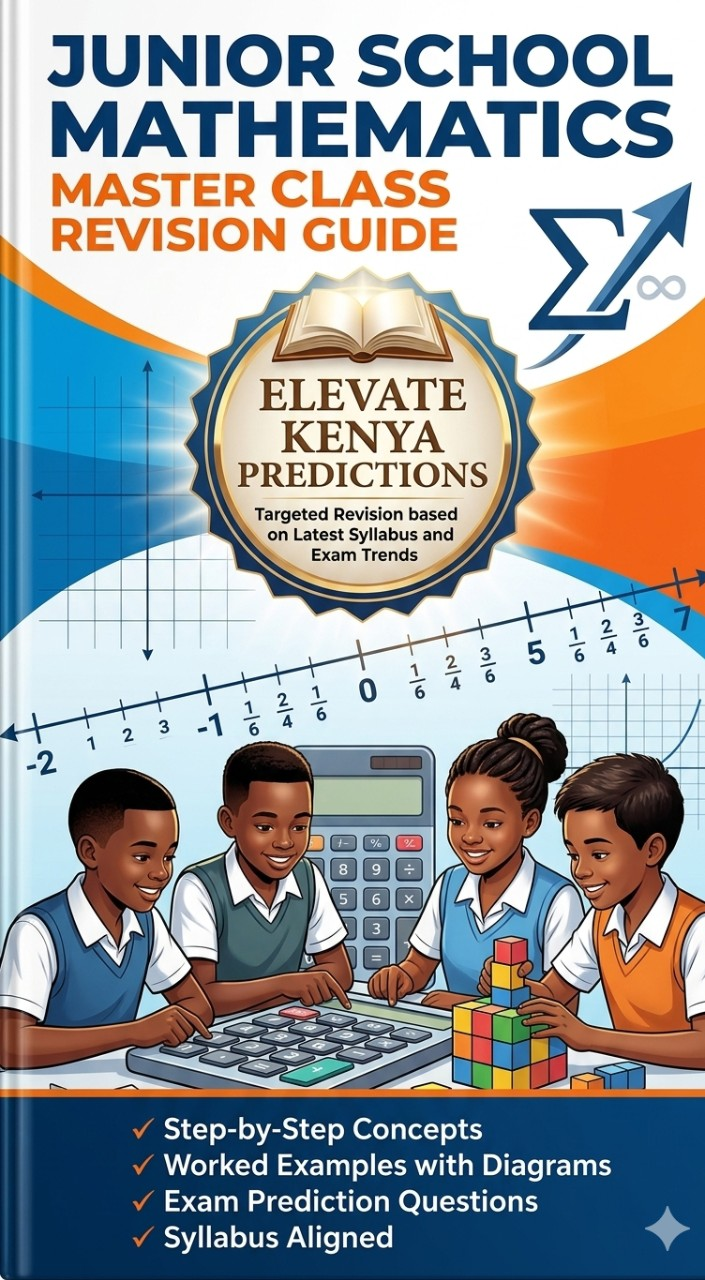
\includegraphics[width=\paperwidth, height=\paperheight]{cover.jpg}%
}{%
    \centering
    \vspace*{10cm} 
    \Huge \textbf{\color{primaryblue}MASTER CLASS: MATHEMATICS} \\ 
    \Large Elevation Pillar \\
}
\end{minipage}
\restoregeometry
\clearpage

% --- 2. TABLE OF CONTENTS ---
\newgeometry{margin=2cm, top=1.5cm, bottom=2cm}
\pagenumbering{roman}
\setcounter{page}{1}
\pagestyle{plain}

\begin{center}
    \begin{tcolorbox}[colback=primaryblue, colframe=primaryblue, arc=0pt, center title, width=\textwidth]
        \color{white}\Large\bfseries TABLE OF CONTENTS
    \end{tcolorbox}
\end{center}

\vspace{0.2cm}

\addcontentsline{toc}{section}{1.0 Numbers}
\addcontentsline{toc}{subsection}{Whole numbers}
\addcontentsline{toc}{subsection}{Factors}
\addcontentsline{toc}{subsection}{Fractions}
\addcontentsline{toc}{subsection}{Decimals}
\addcontentsline{toc}{subsection}{Squares and square roots}
\addcontentsline{toc}{subsection}{Integers}
\addcontentsline{toc}{subsection}{Cubes and cube roots}
\addcontentsline{toc}{subsection}{Rates, ratio, proportions and percentages}
\addcontentsline{toc}{subsection}{Indices and logarithms}

\addcontentsline{toc}{section}{2.0 Algebra}
\addcontentsline{toc}{subsection}{Algebraic expressions}
\addcontentsline{toc}{subsection}{Linear equations}
\addcontentsline{toc}{subsection}{Linear inequalities}
\addcontentsline{toc}{subsection}{Equation of a straight line}
\addcontentsline{toc}{subsection}{Matrices}

\addcontentsline{toc}{section}{3.0 Measurements}
\addcontentsline{toc}{subsection}{Pythagorean relationship}
\addcontentsline{toc}{subsection}{Length}
\addcontentsline{toc}{subsection}{Circles}
\addcontentsline{toc}{subsection}{Area}
\addcontentsline{toc}{subsection}{Volume and capacity}
\addcontentsline{toc}{subsection}{Mass, volume, weight and density}
\addcontentsline{toc}{subsection}{Time, distance and speed}
\addcontentsline{toc}{subsection}{Temperature}
\addcontentsline{toc}{subsection}{Money}
\addcontentsline{toc}{subsection}{Approximation and errors}

\addcontentsline{toc}{section}{4.0 Geometry}
\addcontentsline{toc}{subsection}{Angles}
\addcontentsline{toc}{subsection}{Geometrical constructions}
\addcontentsline{toc}{subsection}{Coordinates and graphs}
\addcontentsline{toc}{subsection}{Scale drawing}
\addcontentsline{toc}{subsection}{Common solids}
\addcontentsline{toc}{subsection}{Similarity and enlargement}
\addcontentsline{toc}{subsection}{Trigonometry}

\addcontentsline{toc}{section}{5.0 Data handling and probability}
\addcontentsline{toc}{subsection}{Data handling}
\addcontentsline{toc}{subsection}{Data presentation and interpretation}
\addcontentsline{toc}{subsection}{Data interpretation (Grouped Data)}
\addcontentsline{toc}{subsection}{Probability}

\vspace{10pt}
\addcontentsline{toc}{section}{KJSEA SAMPLE PAPERS}
\addcontentsline{toc}{section}{MARKING SCHEME}

\tableofcontents
\vfill 
\clearpage

% --- 3. CONTENT AREA ---
\pagenumbering{arabic}
\setcounter{page}{1}
\pagestyle{contentpages}

% --- 3. START CONTENT ---
\pagenumbering{arabic}
\setcounter{page}{1} 
\pagestyle{contentpages}

\begin{center}
    \begin{tcolorbox}[colback=strandcolor!10, colframe=strandcolor, width=0.6\textwidth, arc=10pt, center title]
        \centering \Large \bfseries \color{strandcolor} 1.0 NUMBERS
    \end{tcolorbox}
\end{center}

\section*{1.1 Place Value and Total Value}

\begin{tcolorbox}[colback=lightgrey, colframe=primaryblue, title=\textbf{Concept Summary}, arc=5pt]
    \textbf{Place Value:} Refers to the \textit{name of the position} a digit occupies in a number. \\
    \textbf{Total Value:} Refers to the \textit{numerical worth} of a digit based on its position. \\
    \textbf{Formula:} $\text{Total Value} = \text{Digit} \times \text{Place Value Representation}$
    
    \vspace{5pt}
    \centering
    \small
    \begin{tabularx}{\textwidth}{|X|c|c|c|c|c|c|c|}
    \hline
    \textbf{Digit} & 7 & 4 & 1 & 0 & 3 & 9 & 5 \\ \hline
    \textbf{Place Value} & Millions & H-Th & T-Th & Th & H & T & O \\ \hline
    \end{tabularx}
\end{tcolorbox}

\subsection*{Assessment Exercises (Mastery Level)}

\begin{solvingbox}{Question 1 (Place Value)}
Identify the \textbf{place value} of digit 6 in the number \textbf{8,642,105}. \\
Place Value = \textbf{Hundred Thousands} \hfill $A_1$
\end{solvingbox}

\begin{solvingbox}{Question 2 (Place Value)}
In the number \textbf{14.785}, what is the \textbf{place value} of the digit 8? \\
Place Value = \textbf{Hundredths} \hfill $A_1$
\end{solvingbox}

\begin{solvingbox}{Question 3 (Place Value)}
A farmer harvested \textbf{7,204,318} bags of maize. Which digit occupies the \textbf{Millions} position in this number? \\
The digit is \textbf{7}. \hfill $A_1$
\end{solvingbox}

\begin{solvingbox}{Question 4 (Place Value)}
Which digit has a \textbf{larger} place value in the number \textbf{3,905}; the digit 3 or the digit 9? Explain. \\
Digit \textbf{3}. It is in the \textbf{Thousands} position, while 9 is in the \textbf{Hundreds} position. \hfill $A_1$
\end{solvingbox}

\begin{solvingbox}{Question 5 (Place Value)}
Write the \textbf{place value} of the underlined digit in \textbf{4\underline{5},296,000}. \\
Place Value = \textbf{Millions} \hfill $A_1$
\end{solvingbox}

\newpage

\begin{solvingbox}{Question 6 (Total Value)}
In the number \textbf{9,403,617}, calculate the \textbf{sum} of the total values of digits 9 and 3. \\
TV of 9 = $9,000,000$; TV of 3 = $3,000$ \hfill $M_1$ \\
Sum = $9,000,000 + 3,000 = \mathbf{9,003,000}$ \hfill $A_1$
\end{solvingbox}

\begin{solvingbox}{Question 7 (Total Value)}
\textbf{How much more} is the total value of digit 8 than the total value of digit 5 in \textbf{48,502,963}? \\
TV 8 = $8,000,000$; TV 5 = $500,000$ \hfill $M_1$ \\
Difference = $8,000,000 - 500,000 = \mathbf{7,500,000}$ \hfill $A_1$
\end{solvingbox}

\begin{solvingbox}{Question 8 (Total Value)}
In the number \textbf{720,485}, \textbf{how many times} is the total value of digit 2 greater than the total value of digit 4? \\
TV 2 = $20,000$; TV 4 = $400$ \hfill $M_1$ \\
Ratio = $20,000 \div 400 = \mathbf{50}$ \textbf{times} \hfill $A_1$
\end{solvingbox}

\begin{solvingbox}{Question 9 (Total Value)}
Work out the \textbf{quotient} when the total value of digit 6 is divided by the total value of digit 4 in the number \textbf{15,640,000}. \\
TV 6 = $600,000$; TV 4 = $40,000$ \hfill $M_1$ \\
Quotient = $600,000 \div 40,000 = \mathbf{15}$ \hfill $A_1$
\end{solvingbox}

\begin{solvingbox}{Question 10 (Total Value)}
Find the \textbf{difference} between the total values of the two digits 9 in the number \textbf{904,900}. \\
TV of 1st 9 = $900,000$; TV of 2nd 9 = $900$ \hfill $M_1$ \\
Difference = $900,000 - 900 = \mathbf{899,100}$ \hfill $A_1$
\end{solvingbox}

\begin{solvingbox}{Question 11 (Total Value)}
A company's profit was \textbf{Sh. 74,103,589}. \textbf{How much more} is the total value of digit 7 than the total value of digit 4? \\
TV 7 = $70,000,000$; TV 4 = $4,000,000$ \hfill $M_1$ \\
Difference = $70,000,000 - 4,000,000 = \mathbf{66,000,000}$ \hfill $A_1$
\end{solvingbox}

\begin{solvingbox}{Question 12 (Total Value)}
Calculate the \textbf{sum} of the total value of digit 5 and digit 2 in the number \textbf{5,020}. \\
TV 5 = $5,000$; TV 2 = $20$ \hfill $M_1$ \\
Sum = $5,000 + 20 = \mathbf{5,020}$ \hfill $A_1$
\end{solvingbox}

\section*{1.1.2 Writing Numbers in Words and Numerals}

\begin{tcolorbox}[colback=lightgrey, colframe=primaryblue, title=\textbf{Concept Summary}, arc=5pt]
    \textbf{Numerals to Words:} To write numbers in words, group the digits into periods of threes (ones, thousands, millions) starting from the right. Use a comma to separate these periods. \\
    \textbf{Words to Numerals:} Identify the place value keywords (e.g., "Million", "Thousand") and place the digits in their respective positions. Use zeros as placeholders for any missing place values.
    
    \textbf{Example:} \textit{Nine million, four hundred and five thousand, and twenty-one.} \\
    \textbf{Numeral:} 9,405,021
\end{tcolorbox}

\subsection*{Assessment Exercises (Mastery Level)}

\begin{solvingbox}{Question 1 (Words to Numerals)}
A government project in Kenya was funded to the tune of \textbf{eighty-six million, four hundred and seventy-two thousand, nine hundred and five} shillings. Represent this amount in symbols. \\
Millions: 86; Thousands: 472; Ones: 905 \hfill $M_1$ \\
Numeral = \textbf{Sh. 86,472,905} \hfill $A_1$
\end{solvingbox}

\begin{solvingbox}{Question 2 (Words to Numerals)}
The population of a certain country is estimated to be \textbf{five million, six hundred thousand and forty-two}. Write this population in figures. \\
Millions: 5; Thousands: 600; Ones: 042 \hfill $M_1$ \\
Numeral = \textbf{5,600,042} \hfill $A_1$
\end{solvingbox}

\begin{solvingbox}{Question 3 (Words to Numerals)}
A company produced \textbf{twelve million, eight thousand and seven} bottle tops in a year. How is this number written in numerals? \\
Millions: 12; Thousands: 008; Ones: 007 \hfill $M_1$ \\
Numeral = \textbf{12,008,007} \hfill $A_1$
\end{solvingbox}

\begin{solvingbox}{Question 4 (Words to Numerals)}
Write the following number in symbols: \textbf{nine hundred and ninety-nine million, nine hundred and ninety thousand}. \\
Millions: 999; Thousands: 990; Ones: 000 \hfill $M_1$ \\
Numeral = \textbf{999,990,000} \hfill $A_1$
\end{solvingbox}

\begin{solvingbox}{Question 5 (Words to Numerals)}
A coffee factory processed \textbf{sixteen million, four hundred and twelve thousand and eleven} kilograms of berries. Represent this weight in numerals. \\
Millions: 16; Thousands: 412; Ones: 011 \hfill $M_1$ \\
Numeral = \textbf{16,412,011} \hfill $A_1$
\end{solvingbox}

\begin{solvingbox}{Question 6 (Words to Numerals)}
What is \textbf{three million, three thousand and three} written in figures? \\
Millions: 3; Thousands: 003; Ones: 003 \hfill $M_1$ \\
Numeral = \textbf{3,003,003} \hfill $A_1$
\end{solvingbox}


\begin{solvingbox}{Question 7 (Numerals to Words)}
A national park recorded a total of \textbf{4,050,712} tourists over a decade. Write the number of tourists in words. \\
4 - Millions; 050 - Fifty Thousand; 712 - Seven hundred and twelve \hfill $M_1$ \\
Words: \textbf{Four million, fifty thousand, seven hundred and twelve.} \hfill $A_1$
\end{solvingbox}

\begin{solvingbox}{Question 8 (Numerals to Words)}
The total value of all shares in a cooperative society is \textbf{Sh. 702,008,940}. How would you read this amount in words? \\
702 - Seven hundred and two million; 008 - Eight thousand; 940 - Nine hundred and forty \hfill $M_1$ \\
Words: \textbf{Seven hundred and two million, eight thousand, nine hundred and forty.} \hfill $A_1$
\end{solvingbox}

\begin{solvingbox}{Question 9 (Numerals to Words)}
During a census, the number of school-going children was found to be \textbf{15,000,405}. Express this figure in words. \\
15 - Fifteen million; 000 - Zero thousands; 405 - Four hundred and five \hfill $M_1$ \\
Words: \textbf{Fifteen million, four hundred and five.} \hfill $A_1$
\end{solvingbox}

\begin{solvingbox}{Question 10 (Numerals to Words)}
A construction project used \textbf{1,230,000} bricks. Write the number of bricks used in words. \\
1 - One million; 230 - Two hundred and thirty thousand \hfill $M_1$ \\
Words: \textbf{One million, two hundred and thirty thousand.} \hfill $A_1$
\end{solvingbox}

\begin{solvingbox}{Question 11 (Numerals to Words)}
Express the number \textbf{98,004,001} in words. \\
98 - Ninety-eight million; 004 - Four thousand; 001 - One \hfill $M_1$ \\
Words: \textbf{Ninety-eight million, four thousand and one.} \hfill $A_1$
\end{solvingbox}

\begin{solvingbox}{Question 12 (Numerals to Words)}
In a digital competition, the winner received \textbf{6,700,080} votes. Write the number of votes in words. \\
6 - Six million; 700 - Seven hundred thousand; 080 - Eighty \hfill $M_1$ \\
Words: \textbf{Six million, seven hundred thousand and eighty.} \hfill $A_1$
\end{solvingbox}

\section*{1.1.3 Rounding off numbers}

\begin{tcolorbox}[colback=lightgrey, colframe=primaryblue, title=\textbf{Concept Summary}, arc=5pt]
    Rounding off is the process of replacing a number with a simpler value that is approximately equal to it. \\
    
    \textbf{Rules for Rounding:}
    \begin{enumerate}
        \item Identify the \textbf{rounding digit} (the place value you are rounding to).
        \item Look at the digit to its \textbf{immediate right} (the deciding digit).
        \item If the deciding digit is \textbf{5 or more}, add 1 to the rounding digit (\textbf{Round Up}).
        \item If the deciding digit is \textbf{less than 5}, the rounding digit remains the same (\textbf{Round Down}).
        \item Change all digits to the right of the rounding digit to \textbf{zeros}.
    \end{enumerate}
\end{tcolorbox}

\subsection*{Assessment Exercises (Mastery Level)}

\begin{solvingbox}{Question 1 (Rounding to Thousands)}
A tea factory produced \textbf{48,725 kg} of tea leaves. Round off the amount to the \textbf{nearest thousand}. \\
Rounding digit (Thousands) = 8; Deciding digit = 7. \hfill $M_1$ \\
Since 7 $\ge$ 5, we add 1 to 8 to get 9. \hfill $M_1$ \\
Rounded value = \textbf{49,000 kg} \hfill $A_1$
\end{solvingbox}

\begin{solvingbox}{Question 2 (Rounding to Millions)}
A total of \textbf{12,499,300} seedlings were planted. Round off this number to the \textbf{nearest million}. \\
Rounding digit (Millions) = 2; Deciding digit = 4. \hfill $M_1$ \\
Since 4 $<$ 5, the digit 2 remains unchanged. \hfill $M_1$ \\
Rounded value = \textbf{12,000,000 seedlings} \hfill $A_1$
\end{solvingbox}

\begin{solvingbox}{Question 3 (Rounding to Tens)}
A runner covered \textbf{42,195 metres}. Round off this figure to the \textbf{nearest ten}. \\
Rounding digit (Tens) = 9; Deciding digit = 5. \hfill $M_1$ \\
Since the deciding digit is 5, we add 1 to 9 (carrying over). \hfill $M_1$ \\
Rounded value = \textbf{42,200 metres} \hfill $A_1$
\end{solvingbox}

\begin{solvingbox}{Question 4 (Rounding to Nearest Whole Number)}
The mass of a chemical is \textbf{15.74 grams}. Round off to the \textbf{nearest whole number}. \\
Rounding digit (Ones) = 5; Deciding digit (Tenths) = 7. \hfill $M_1$ \\
Since 7 $\ge$ 5, we add 1 to 5. \hfill $M_1$ \\
Rounded value = \textbf{16 grams} \hfill $A_1$
\end{solvingbox}


\begin{solvingbox}{Question 5 (Rounding to Hundreds)}
A school spent \textbf{Sh. 745,862}. Express this expenditure to the \textbf{nearest hundred}. \\
Rounding digit (Hundreds) = 8; Deciding digit = 6. \hfill $M_1$ \\
Since 6 $>$ 5, we round up 8 to 9. \hfill $M_1$ \\
Rounded value = \textbf{Sh. 745,900} \hfill $A_1$
\end{solvingbox}

\begin{solvingbox}{Question 6 (Rounding Decimals)}
The length of a wire is \textbf{8.432 metres}. Round off the length to \textbf{one decimal place}. \\
Rounding digit (Tenths) = 4; Deciding digit (Hundredths) = 3. \hfill $M_1$ \\
Since 3 $<$ 5, the digit 4 remains the same. \hfill $M_1$ \\
Rounded value = \textbf{8.4 metres} \hfill $A_1$
\end{solvingbox}

\begin{solvingbox}{Question 7 (Rounding to Ten Thousands)}
A stadium capacity is \textbf{54,289} people. Round this number to the \textbf{nearest ten thousand}. \\
Rounding digit (Ten Thousands) = 5; Deciding digit = 4. \hfill $M_1$ \\
Since 4 $<$ 5, the 5 remains unchanged. \hfill $M_1$ \\
Rounded value = \textbf{50,000 people} \hfill $A_1$
\end{solvingbox}
\begin{solvingbox}{Question 8 (Rounding to Hundred Thousands)}
A textbook publisher printed \textbf{896,410} copies of a new Mathematics book. Round off the number of copies to the \textbf{nearest hundred thousand}. \\
Rounding digit (Hundred Thousands) = 8; Deciding digit = 9. \hfill $M_1$ \\
Since 9 is greater than 5, we add 1 to 8. \hfill $M_1$ \\
Rounded value = \textbf{900,000 copies} \hfill $A_1$
\end{solvingbox}

\section*{1.1.4 Natural numbers (Odd, Even and Prime Numbers)}

\begin{tcolorbox}[colback=lightgrey, colframe=primaryblue, title=\textbf{Concept Summary}, arc=5pt]
    Natural numbers are counting numbers starting from 1, 2, 3, ... etc. They can be classified based on their properties: \\
    
    \begin{itemize}
        \item \textbf{Even Numbers:} Numbers that are exactly divisible by 2. They end with digits 0, 2, 4, 6, or 8.
        \item \textbf{Odd Numbers:} Numbers that leave a remainder of 1 when divided by 2. They end with digits 1, 3, 5, 7, or 9.
        \item \textbf{Prime Numbers:} Numbers greater than 1 that have exactly two factors: 1 and itself. (Note: 2 is the only even prime number).
    \end{itemize}
\end{tcolorbox}

\subsection*{Assessment Exercises (Mastery Level)}

% --- EVEN NUMBERS (4 Questions) ---
\begin{solvingbox}{Question 1 (Even Numbers)}
A security officer is numbering houses along a street using \textbf{even numbers} only. If the first house is number 102, what will be the number of the \textbf{8th house} in that sequence? \\
Sequence: 102, 104, 106, 108, 110, 112, 114, 116. \hfill $M_1$ \\
The 8th house is number \textbf{116}. \hfill $A_1$
\end{solvingbox}

\begin{solvingbox}{Question 2 (Even Numbers)}
Find the \textbf{sum} of all even numbers between 21 and 31. \\
Even numbers are: 22, 24, 26, 28, 30. \hfill $M_1$ \\
Sum = $22 + 24 + 26 + 28 + 30 = \mathbf{130}$ \hfill $A_1$
\end{solvingbox}

\begin{solvingbox}{Question 3 (Even Numbers)}
A transport company owns a fleet of buses with registration numbers. A technician noted that a certain bus has a 4-digit number where all digits are the \textbf{same even number}, and their \textbf{sum is 24}. Identify the bus number. \\
Let the digit be $x$. $x + x + x + x = 24 \implies 4x = 24$. \hfill $M_1$ \\
$x = 6$. The bus number is \textbf{6,666}. \hfill $A_1$
\end{solvingbox}

\begin{solvingbox}{Question 4 (Even Numbers)}
What is the \textbf{difference} between the largest 3-digit even number and the smallest 2-digit even number? \\
Largest 3-digit even = 998; Smallest 2-digit even = 10. \hfill $M_1$ \\
Difference = $998 - 10 = \mathbf{988}$ \hfill $A_1$
\end{solvingbox}


% --- ODD NUMBERS (4 Questions) ---
\begin{solvingbox}{Question 5 (Odd Numbers)}
A student was asked to list \textbf{five consecutive odd numbers} starting from 45. Calculate the \textbf{average} (mean) of these five numbers. \\
Numbers: 45, 47, 49, 51, 53. \hfill $M_1$ \\
Sum = 245; Mean = $245 \div 5 = \mathbf{49}$ \hfill $A_1$
\end{solvingbox}

\begin{solvingbox}{Question 6 (Odd Numbers)}
Identify the \textbf{largest odd number} that can be formed using the digits \textbf{4, 0, 7, and 5} without repetition. \\
To be odd, it must end in 5 or 7. To be largest, we start with 7. \hfill $M_1$ \\
Possible largest: 7,504 (even), 7,405 (odd), 7,045 (odd). \hfill $M_1$ \\
The largest odd number is \textbf{7,405}. \hfill $A_1$
\end{solvingbox}

\begin{solvingbox}{Question 7 (Odd Numbers)}
Work out the \textbf{product} of the first three odd numbers greater than 10. \\
The numbers are 11, 13, and 15. \hfill $M_1$ \\
Product = $11 \times 13 \times 15 = 143 \times 15 = \mathbf{2,145}$ \hfill $A_1$
\end{solvingbox}

\begin{solvingbox}{Question 8 (Odd Numbers)}
A farmer has \textbf{379} eggs. He wants to pack them in trays of 2. Explain why he will have \textbf{one egg remaining} using the properties of numbers. \\
379 ends in 9, which makes it an \textbf{odd number}. \hfill $M_1$ \\
Odd numbers divided by 2 always leave a \textbf{remainder of 1}. \hfill $A_1$
\end{solvingbox}

% --- PRIME NUMBERS (4 Questions) ---
\begin{solvingbox}{Question 9 (Prime Numbers)}
List all the \textbf{prime numbers} between 70 and 85. \\
Checking: 71, 73, 79, 83. \hfill $M_1$ \\
The prime numbers are \textbf{71, 73, 79, and 83}. \hfill $A_1$
\end{solvingbox}

\begin{solvingbox}{Question 10 (Prime Numbers)}
Find the \textbf{sum} of the first five prime numbers. \\
Prime numbers: 2, 3, 5, 7, 11. \hfill $M_1$ \\
Sum = $2 + 3 + 5 + 7 + 11 = \mathbf{28}$ \hfill $A_1$
\end{solvingbox}

\begin{solvingbox}{Question 11 (Prime Numbers)}
A secret code is formed by multiplying the \textbf{only even prime number} by the \textbf{next two consecutive prime numbers}. What is the code? \\
Even prime = 2; Next two primes = 3 and 5. \hfill $M_1$ \\
Code = $2 \times 3 \times 5 = \mathbf{30}$ \hfill $A_1$
\end{solvingbox}

\begin{solvingbox}{Question 12 (Prime Numbers)}
Is the number \textbf{91} a prime number? Show your working by listing its factors. \\
Factors of 91: 1, 7, 13, 91. \hfill $M_1$ \\
Since it has \textbf{more than two factors} (it is divisible by 7 and 13), it is \textbf{not} a prime number. \hfill $A_1$
\end{solvingbox}

\section*{1.1.5 Operations: Addition and Subtraction}

\begin{tcolorbox}[colback=lightgrey, colframe=primaryblue, title=\textbf{Concept Summary}, arc=5pt]
    \textbf{Addition:} The process of calculating the total of two or more numbers. Key terms include \textit{Sum, Total, Increase,} and \textit{Altogether}. When adding, align digits according to their place values and carry over where the sum exceeds 9. \\
    
    \textbf{Subtraction:} The process of taking one number away from another to find the \textit{Difference, Remainder,} or \textit{Balance}. Always subtract the smaller number from the larger one, aligning place values and borrowing from the next higher value when necessary.
\end{tcolorbox}

\subsection*{Assessment Exercises (Mastery Level)}

\begin{center}
    \textbf{\color{strandcolor} SECTION A: ADDITION}
\end{center}

\begin{solvingbox}{Question 1 (Addition)}
In a certain county, the number of Grade 7 students is \textbf{456,780} and the number of Grade 8 students is \textbf{398,450}. What is the total number of students in both grades? \\
Aligning place values: \\
\phantom{+} 456,780 \\
+ 398,450 \hfill $M_1$ \\
\rule{2.5cm}{0.4pt} \\
\textbf{855,230} \hfill $A_1$ \\
The total number of students is \textbf{855,230}.
\end{solvingbox}

\begin{solvingbox}{Question 2 (Addition)}
A milk processing plant produced \textbf{1,245,600 litres} in January and \textbf{987,550 litres} in February. Calculate the total volume of milk produced in the two months. \\
Total = $1,245,600 + 987,550$ \hfill $M_1$ \\
\phantom{+} 1,245,600 \\
+ \phantom{1,}987,550 \hfill $M_1$ \\
\rule{2.5cm}{0.4pt} \\
\textbf{2,233,150} \hfill $A_1$ \\
The total volume is \textbf{2,233,150 litres}.
\end{solvingbox}

\begin{solvingbox}{Question 3 (Addition)}
A construction company bought three parcels of land for \textbf{Sh. 15,450,000}, \textbf{Sh. 8,200,500}, and \textbf{Sh. 12,750,000}. Find the total cost of the three parcels. \\
Sum = $15,450,000 + 8,200,500 + 12,750,000$ \hfill $M_1$ \\
\phantom{+} 15,450,000 \\
\phantom{+} 08,200,500 \\
+ 12,750,000 \hfill $M_1$ \\
\rule{2.5cm}{0.4pt} \\
\textbf{36,400,500} \hfill $A_1$ \\
The total cost is \textbf{Sh. 36,400,500}.
\end{solvingbox}

\begin{solvingbox}{Question 4 (Addition)}
A certain year, a forest department planted \textbf{2,345,678} indigenous trees and \textbf{1,567,890} exotic trees. How many trees were planted altogether? \\
Indigenous: 2,345,678; Exotic: 1,567,890 \hfill $M_1$ \\
Total: $2,345,678 + 1,567,890 = \mathbf{3,913,568}$ \hfill $A_1$ \\
A total of \textbf{3,913,568 trees} were planted.
\end{solvingbox}

\begin{solvingbox}{Question 5 (Addition)}
A wholesale trader sold \textbf{56,780 bags} of maize in the first quarter, \textbf{43,210 bags} in the second quarter, and \textbf{65,900 bags} in the third quarter. Work out the total sales. \\
Total = $56,780 + 43,210 + 65,900$ \hfill $M_1$ \\
Sum = \textbf{165,890} \hfill $A_1$ \\
The total sales were \textbf{165,890 bags}.
\end{solvingbox}

\begin{solvingbox}{Question 6 (Addition)}
The mass of three containers is \textbf{12,450 kg}, \textbf{9,780 kg}, and \textbf{15,600 kg}. Find the total mass of the three containers. \\
Total mass = $12,450 + 9,780 + 15,600$ \hfill $M_1$ \\
Sum = \textbf{37,830} \hfill $A_1$ \\
The total mass is \textbf{37,830 kg}.
\end{solvingbox}

\begin{solvingbox}{Question 7 (Addition)}
An election candidate received \textbf{45,670 votes} in one constituency and \textbf{38,940 votes} in another. How many votes did the candidate receive in total? \\
Total votes = $45,670 + 38,940$ \hfill $M_1$ \\
Sum = \textbf{84,610} \hfill $A_1$ \\
The total number of votes is \textbf{84,610}.
\end{solvingbox}

\begin{solvingbox}{Question 8 (Addition)}
A digital library has \textbf{1,234,500 books} in English and \textbf{876,400 books} in Swahili. Find the total number of books in the library. \\
Total = $1,234,500 + 876,400$ \hfill $M_1$ \\
Sum = \textbf{2,110,900} \hfill $A_1$ \\
The library has \textbf{2,110,900 books}.
\end{solvingbox}


\begin{center}
    \textbf{\color{strandcolor} SECTION B: SUBTRACTION}
\end{center}

\begin{solvingbox}{Question 1 (Subtraction)}
A coffee cooperative society had \textbf{Sh. 45,670,800} in its bank account. After paying farmers, the balance was \textbf{Sh. 12,345,600}. How much money was paid to the farmers? \\
Amount paid = Initial Amount - Balance \hfill $M_1$ \\
\phantom{-} 45,670,800 \\
- 12,345,600 \hfill $M_1$ \\
\rule{2.5cm}{0.4pt} \\
\textbf{33,325,200} \hfill $A_1$ \\
The amount paid was \textbf{Sh. 33,325,200}.
\end{solvingbox}

\begin{solvingbox}{Question 2 (Subtraction)}
The target for a dam construction was to hold \textbf{5,000,000 cubic metres} of water. Currently, it holds \textbf{2,450,750 cubic metres}. What is the remaining volume needed to fill the dam? \\
Difference = $5,000,000 - 2,450,750$ \hfill $M_1$ \\
\phantom{-} 5,000,000 \\
- 2,450,750 \hfill $M_1$ \\
\rule{2.5cm}{0.4pt} \\
\textbf{2,549,250} \hfill $A_1$ \\
The remaining volume is \textbf{2,549,250 $m^3$}.
\end{solvingbox}

\begin{solvingbox}{Question 3 (Subtraction)}
A town has a population of \textbf{896,400}. If there are \textbf{452,150 males}, find the number of females in the town. \\
Females = Total Population - Males \hfill $M_1$ \\
\phantom{-} 896,400 \\
- 452,150 \hfill $M_1$ \\
\rule{2.5cm}{0.4pt} \\
\textbf{444,250} \hfill $A_1$ \\
The number of females is \textbf{444,250}.
\end{solvingbox}

\begin{solvingbox}{Question 4 (Subtraction)}
Subtract \textbf{987,654} from \textbf{2,000,000}. \\
Calculation: $2,000,000 - 987,654$ \hfill $M_1$ \\
Difference = \textbf{1,012,346} \hfill $A_1$
\end{solvingbox}

\begin{solvingbox}{Question 5 (Subtraction)}
A lorry carried \textbf{25,000 kg} of cement. After offloading some bags at a hardware shop, \textbf{12,450 kg} remained. What was the mass of cement offloaded? \\
Offloaded = $25,000 - 12,450$ \hfill $M_1$ \\
Difference = \textbf{12,550} \hfill $A_1$ \\
The mass offloaded was \textbf{12,550 kg}.
\end{solvingbox}

\begin{solvingbox}{Question 6 (Subtraction)}
The price of a house dropped from \textbf{Sh. 12,500,000} to \textbf{Sh. 9,750,000}. By how much did the price decrease? \\
Decrease = $12,500,000 - 9,750,000$ \hfill $M_1$ \\
Difference = \textbf{2,750,000} \hfill $A_1$ \\
The price decreased by \textbf{Sh. 2,750,000}.
\end{solvingbox}

\begin{solvingbox}{Question 7 (Subtraction)}
A student needs \textbf{Sh. 85,600} for school fees. He has \textbf{Sh. 32,450} in his savings. How much more money does he need? \\
Balance needed = $85,600 - 32,450$ \hfill $M_1$ \\
Difference = \textbf{53,150} \hfill $A_1$ \\
He needs \textbf{Sh. 53,150 more}.
\end{solvingbox}

\begin{solvingbox}{Question 8 (Subtraction)}
What is the \textbf{difference} between the largest 7-digit number and the smallest 7-digit number? \\
Largest = 9,999,999; Smallest = 1,000,000 \hfill $M_1$ \\
Difference = \textbf{8,999,999} \hfill $A_1$
\end{solvingbox}

\section*{1.1.5 Operations: Multiplication and Division}

\begin{tcolorbox}[colback=lightgrey, colframe=primaryblue, title=\textbf{Concept Summary}, arc=5pt]
    \textbf{Multiplication:} This is the process of repeated addition. The result of multiplying two or more numbers is called the \textit{Product}. Key strategies include long multiplication, where digits are multiplied by place value starting from the ones. \\
    
    \textbf{Division:} This is the process of sharing or grouping a number into equal parts. The number being divided is the \textit{Dividend}, the number dividing is the \textit{Divisor}, and the result is the \textit{Quotient}. Any left-over value is the \textit{Remainder}.
\end{tcolorbox}

\subsection*{Assessment Exercises (Mastery Level)}

\begin{center}
    \textbf{\color{strandcolor} SECTION C: MULTIPLICATION}
\end{center}

\begin{solvingbox}{Question 1 (Multiplication)}
A primary school has \textbf{15 classes}, and each class has \textbf{45 students}. How many students are there in the school altogether? \\
Total students = $15 \times 45$ \hfill $M_1$ \\
$45 \times 10 = 450$; $45 \times 5 = 225$ \hfill $M_1$ \\
$450 + 225 = \mathbf{675}$ \hfill $A_1$ \\
There are \textbf{675 students} in the school.
\end{solvingbox}

\begin{solvingbox}{Question 2 (Multiplication)}
A farmer harvests \textbf{120 bags} of maize. If each bag weighs \textbf{90 kg}, find the total weight of the harvest. \\
Total weight = $120 \times 90$ \hfill $M_1$ \\
$12 \times 9 = 108$; add two zeros $\implies 10,800$ \hfill $M_1$ \\
Total weight = \textbf{10,800 kg} \hfill $A_1$
\end{solvingbox}

\begin{solvingbox}{Question 3 (Multiplication)}
A factory produces \textbf{2,450 bottles} of soda every hour. How many bottles will be produced if the factory runs for \textbf{8 hours}? \\
Total bottles = $2,450 \times 8$ \hfill $M_1$ \\
$2,450 \times 8 = \mathbf{19,600}$ \hfill $A_1$ \\
The factory will produce \textbf{19,600 bottles}.
\end{solvingbox}

\begin{solvingbox}{Question 4 (Multiplication)}
A trader buys \textbf{25 cartons} of books. Each carton contains \textbf{48 books}. Calculate the total number of books bought. \\
Total books = $25 \times 48$ \hfill $M_1$ \\
$25 \times 4 \times 12 = 100 \times 12 = \mathbf{1,200}$ \hfill $M_1$ \\
Total books = \textbf{1,200} \hfill $A_1$
\end{solvingbox}

\begin{solvingbox}{Question 5 (Multiplication)}
If a bus travels \textbf{75 km in one hour}, what distance will it cover in \textbf{12 hours} at the same speed? \\
Distance = $75 \times 12$ \hfill $M_1$ \\
$75 \times 10 = 750$; $75 \times 2 = 150$ \hfill $M_1$ \\
$750 + 150 = \mathbf{900}$ \hfill $A_1$ \\
The bus covers \textbf{900 km}.
\end{solvingbox}

\begin{solvingbox}{Question 6 (Multiplication)}
A company pays a casual worker \textbf{Sh. 850 per day}. How much will the worker earn after working for \textbf{26 days}? \\
Earnings = $850 \times 26$ \hfill $M_1$ \\
$850 \times 26 = \mathbf{22,100}$ \hfill $A_1$ \\
The worker earns \textbf{Sh. 22,100}.
\end{solvingbox}

\begin{solvingbox}{Question 7 (Multiplication)}
Calculate the product of \textbf{1,234} and \textbf{56}. \\
$1,234 \times 50 = 61,700$ \\
$1,234 \times 6 = 7,404$ \hfill $M_1$ \\
$61,700 + 7,404 = \mathbf{69,104}$ \hfill $A_1$
\end{solvingbox}

\begin{solvingbox}{Question 8 (Multiplication)}
A rectangular plot of land measures \textbf{45 metres by 30 metres}. Find its area in square metres. \\
Area = Length $\times$ Width \hfill $M_1$ \\
Area = $45 \times 30 = \mathbf{1,350}$ \hfill $A_1$ \\
The area is \textbf{1,350 $m^2$}.
\end{solvingbox}

\begin{solvingbox}{Question 9 (Multiplication)}
A wholesaler sells \textbf{150 crates} of eggs. Each crate has \textbf{30 eggs}. How many eggs are sold in total? \\
Total eggs = $150 \times 30$ \hfill $M_1$ \\
$15 \times 3 = 45$; add two zeros $\implies 4,500$ \hfill $M_1$ \\
Total = \textbf{4,500 eggs} \hfill $A_1$
\end{solvingbox}

\begin{solvingbox}{Question 10 (Multiplication)}
What is the product of the largest 3-digit number and the smallest 2-digit number? \\
Largest 3-digit = 999; Smallest 2-digit = 10 \hfill $M_1$ \\
Product = $999 \times 10 = \mathbf{9,990}$ \hfill $A_1$
\end{solvingbox}
\newpage

% --- DIVISION (10 Questions) ---
\begin{center}
    \textbf{\color{strandcolor} SECTION D: DIVISION}
\end{center}

\begin{solvingbox}{Question 1 (Division)}
A prize of \textbf{Sh. 45,000} is shared equally among \textbf{9 winners}. How much does each winner receive? \\
Each share = $45,000 \div 9$ \hfill $M_1$ \\
$45 \div 9 = 5$; add three zeros $\implies 5,000$ \hfill $M_1$ \\
Each winner receives \textbf{Sh. 5,000} \hfill $A_1$
\end{solvingbox}

\begin{solvingbox}{Question 2 (Division)}
A library has \textbf{1,200 books} to be placed on \textbf{40 shelves}. If each shelf holds an equal number of books, how many books are on each shelf? \\
Books per shelf = $1,200 \div 40$ \hfill $M_1$ \\
$120 \div 4 = 30$ \hfill $M_1$ \\
Each shelf has \textbf{30 books}. \hfill $A_1$
\end{solvingbox}

\begin{solvingbox}{Question 3 (Division)}
Divide \textbf{1,452} by \textbf{12}. \\
$144 \div 12 = 12$; $12 \div 12 = 1$ \hfill $M_1$ \\
Quotient = \textbf{121} \hfill $A_1$
\end{solvingbox}

\begin{solvingbox}{Question 4 (Division)}
A tailor uses \textbf{3 metres} of fabric to make one uniform. If he has \textbf{156 metres} of fabric, how many uniforms can he make? \\
Uniforms = $156 \div 3$ \hfill $M_1$ \\
$150 \div 3 = 50$; $6 \div 3 = 2$ \hfill $M_1$ \\
Total = \textbf{52 uniforms} \hfill $A_1$
\end{solvingbox}

\begin{solvingbox}{Question 5 (Division)}
A lorry carries \textbf{9,000 kg} of sand. If the sand is packed into \textbf{50 kg bags}, how many bags will be filled? \\
Number of bags = $9,000 \div 50$ \hfill $M_1$ \\
$900 \div 5 = 180$ \hfill $M_1$ \\
Total = \textbf{180 bags} \hfill $A_1$
\end{solvingbox}

\begin{solvingbox}{Question 6 (Division)}
Work out: \textbf{$4,896 \div 24$}. \\
$48 \div 24 = 2$; $96 \div 24 = 4$ \hfill $M_1$ \\
Quotient = \textbf{204} \hfill $A_1$
\end{solvingbox}

\begin{solvingbox}{Question 7 (Division)}
A school spent \textbf{Sh. 84,000} to buy \textbf{7 identical laptops}. What was the cost of one laptop? \\
Cost per laptop = $84,000 \div 7$ \hfill $M_1$ \\
$84 \div 7 = 12$; add three zeros $\implies 12,000$ \hfill $M_1$ \\
One laptop cost \textbf{Sh. 12,000} \hfill $A_1$
\end{solvingbox}

\begin{solvingbox}{Question 8 (Division)}
A juice dispenser contains \textbf{25,000 ml} of juice. If it is served in \textbf{250 ml cups}, how many cups will be served? \\
Number of cups = $25,000 \div 250$ \hfill $M_1$ \\
$2,500 \div 25 = 100$ \hfill $M_1$ \\
Total = \textbf{100 cups} \hfill $A_1$
\end{solvingbox}

\begin{solvingbox}{Question 9 (Division)}
Find the quotient and the remainder when \textbf{507} is divided by \textbf{8}. \\
$50 \div 8 = 6$ rem 2; $27 \div 8 = 3$ rem 3 \hfill $M_1$ \\
Quotient = \textbf{63}, Remainder = \textbf{3} \hfill $A_1$
\end{solvingbox}

\begin{solvingbox}{Question 10 (Division)}
A group of \textbf{15 friends} contributed an equal amount to raise \textbf{Sh. 18,750} for a charity. How much did each friend contribute? \\
Contribution = $18,750 \div 15$ \hfill $M_1$ \\
$1,875 \div 15 = 125$; add zero $\implies 1,250$ \hfill $M_1$ \\
Each friend contributed \textbf{Sh. 1,250} \hfill $A_1$
\end{solvingbox}

\section*{1.2.1 Divisibility Test}

\begin{tcolorbox}[colback=lightgrey, colframe=primaryblue, title=\textbf{Concept Summary}, arc=5pt]
    Divisibility tests are shortcut rules used to determine whether a whole number is divisible by a fixed divisor without performing the actual long division.
    
    \begin{itemize}
        \item \textbf{Divisibility by 2:} The last digit must be even (0, 2, 4, 6, or 8).
        \item \textbf{Divisibility by 3:} The sum of all digits must be divisible by 3.
        \item \textbf{Divisibility by 4:} The number formed by the last two digits must be divisible by 4.
        \item \textbf{Divisibility by 5:} The last digit must be 0 or 5.
        \item \textbf{Divisibility by 6:} The number must be divisible by \textbf{both} 2 and 3.
        \item \textbf{Divisibility by 8:} The number formed by the last three digits must be divisible by 8.
        \item \textbf{Divisibility by 9:} The sum of all digits must be divisible by 9.
        \item \textbf{Divisibility by 10:} The last digit must be 0.
        \item \textbf{Divisibility by 11:} The difference between the sum of digits in odd positions and even positions must be 0 or a multiple of 11.
    \end{itemize}
\end{tcolorbox}

\subsection*{Assessment Exercises (Mastery Level)}

\begin{solvingbox}{Question 1 (Divisibility by 3)}
A student is given the number \textbf{4,563}. Without dividing, determine if the number is divisible by 3. \\
Sum of digits = $4 + 5 + 6 + 3 = 18$. \hfill $M_1$ \\
Since 18 is a multiple of 3 ($3 \times 6 = 18$), the number is \textbf{divisible by 3}. \hfill $A_1$
\end{solvingbox}

\begin{solvingbox}{Question 2 (Divisibility by 4)}
Which of the following numbers is divisible by 4? \textbf{7,322} or \textbf{9,136}. Explain using the divisibility rule. \\
Check last two digits: For 7,322, it is 22 (Not divisible by 4). \hfill $M_1$ \\
For 9,136, it is 36 ($4 \times 9 = 36$). \hfill $M_1$ \\
Therefore, \textbf{9,136} is divisible by 4. \hfill $A_1$
\end{solvingbox}

\begin{solvingbox}{Question 3 (Divisibility by 6)}
Test if the number \textbf{816} is divisible by 6. \\
Rule: Must be divisible by 2 and 3. \hfill $M_1$ \\
Divisible by 2? Yes (ends in 6). Divisible by 3? Yes ($8+1+6=15$, which is divisible by 3). \hfill $M_1$ \\
Since it satisfies both, \textbf{816 is divisible by 6}. \hfill $A_1$
\end{solvingbox}

\begin{solvingbox}{Question 4 (Divisibility by 8)}
A container has \textbf{15,824} bottle tops. Can these be shared equally among 8 children without a remainder? \\
Check last three digits: 824. \hfill $M_1$ \\
$824 \div 8 = 103$. Since 824 is divisible by 8, then \textbf{15,824 is divisible by 8}. \hfill $A_1$
\end{solvingbox}

\begin{solvingbox}{Question 5 (Divisibility by 9)}
Find the smallest digit that can be placed in the box $\square$ to make \textbf{7,2$\square$5} divisible by 9. \\
Sum of known digits = $7 + 2 + 5 = 14$. \hfill $M_1$ \\
Next multiple of 9 after 14 is 18. \hfill $M_1$ \\
Missing digit = $18 - 14 = \mathbf{4}$. \hfill $A_1$
\end{solvingbox}

\begin{solvingbox}{Question 6 (Divisibility by 11)}
Test if the number \textbf{91,806} is divisible by 11. \\
Sum of digits in odd positions (1st, 3rd, 5th): $9 + 8 + 6 = 23$. \hfill $M_1$ \\
Sum of digits in even positions (2nd, 4th): $1 + 0 = 1$. \hfill $M_1$ \\
Difference = $23 - 1 = 22$. Since 22 is a multiple of 11, \textbf{91,806 is divisible by 11}. \hfill $A_1$
\end{solvingbox}

\begin{solvingbox}{Question 7 (Divisibility by 5 and 10)}
State two properties that a number must have to be divisible by \textbf{both 5 and 10}. \\
1. The last digit must be 0. \hfill $A_1$ \\
2. It must be an even number. \hfill $A_1$
\end{solvingbox}

\begin{solvingbox}{Question 8 (Divisibility by 2 and 3)}
Is the number \textbf{4,050} divisible by 6? Show your working. \\
Divisible by 2: Yes, it ends in 0. \hfill $M_1$ \\
Divisible by 3: $4+0+5+0 = 9$. 9 is divisible by 3. \hfill $M_1$ \\
Since it is divisible by both 2 and 3, \textbf{it is divisible by 6}. \hfill $A_1$
\end{solvingbox}

\begin{solvingbox}{Question 9 (Divisibility by 4)}
A library has \textbf{1,048} books. The librarian wants to arrange them in sets of 4. Is this possible without a remainder? \\
Last two digits = 48. \hfill $M_1$ \\
$48 \div 4 = 12$. Since 48 is divisible by 4, the total \textbf{is divisible by 4}. \hfill $A_1$
\end{solvingbox}

\begin{solvingbox}{Question 10 (Divisibility by 3 and 9)}
Prove that any number divisible by 9 must also be divisible by 3 using \textbf{729} as an example. \\
$7+2+9 = 18$. 18 is divisible by 9, so 729 is divisible by 9. \hfill $M_1$ \\
Since the sum (18) is also divisible by 3, the number \textbf{must be divisible by 3}. \hfill $A_1$
\end{solvingbox}

\begin{solvingbox}{Question 11 (Divisibility by 11)}
Which digit should be placed at $x$ in \textbf{1x5} to make it divisible by 11? \\
Sum of odd positions: $1 + 5 = 6$. Sum of even: $x$. \hfill $M_1$ \\
For the difference to be 0, $6 - x = 0$. \hfill $M_1$ \\
Therefore, $x = \mathbf{6}$. The number is 165. \hfill $A_1$
\end{solvingbox}

\begin{solvingbox}{Question 12 (Divisibility by 8)}
A worker has \textbf{3,000} bricks. If he arranges them in groups of 8, will he have any bricks left over? \\
Check last three digits: 000. \hfill $M_1$ \\
Rule: Any number ending in three zeros is divisible by 8. \hfill $M_1$ \\
No, there will be \textbf{no bricks left over}. \hfill $A_1$
\end{solvingbox}

\section*{1.2.2 Prime Factors}

\begin{tcolorbox}[colback=lightgrey, colframe=primaryblue, title=\textbf{Concept Summary}, arc=5pt]
    Every natural number greater than 1 is either a prime number or a composite number.
    \begin{itemize}
        \item \textbf{Prime Numbers:} Numbers with exactly two factors (1 and itself). Examples: 2, 3, 5, 7, 11...
        \item \textbf{Composite Numbers:} Numbers with more than two factors. They are formed by multiplying two or more prime numbers. Examples: 4, 6, 8, 9, 10...
    \end{itemize}
    \textbf{Prime Factorization (Decomposition):} This is the process of expressing a composite number as a product of its prime factors. This can be done using a \textbf{Factor Tree} or the \textbf{Division Method}.
\end{tcolorbox}

\subsection*{Example: Factor Tree for 36}
\begin{center}
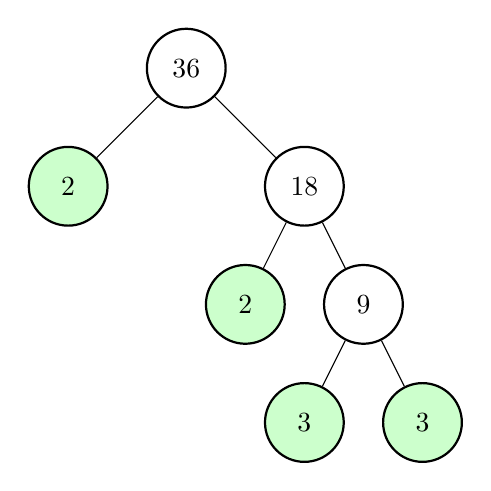
\begin{tikzpicture}[
  level distance=1.5cm,
  level 1/.style={sibling distance=3cm},
  level 2/.style={sibling distance=1.5cm},
  nodes={circle, draw=black, thick, inner sep=2pt, minimum size=1cm}
]
  \node {36}
    child {node [fill=green!20] {2}}
    child {node {18}
      child {node [fill=green!20] {2}}
      child {node {9}
        child {node [fill=green!20] {3}}
        child {node [fill=green!20] {3}}
      }
    };
\end{tikzpicture}
\\ \medskip
\textbf{36 as a product of prime factors:} $2 \times 2 \times 3 \times 3 = 2^2 \times 3^2$
\end{center}

\subsection*{Assessment Exercises (Mastery Level)}

\begin{solvingbox}{Question 1 (Prime vs Composite)}
Which of the following numbers is a \textbf{composite number}? \textbf{17, 21, 23, 29}. Explain your answer. \\
21 is a composite number because it has factors: 1, 3, 7, and 21. \hfill $M_1$ \\
The others are prime numbers with only two factors. \hfill $A_1$
\end{solvingbox}

\begin{solvingbox}{Question 2 (Decomposition)}
Express \textbf{48} as a product of its prime factors in power notation. \\
$48 = 2 \times 24 = 2 \times 2 \times 12 = 2 \times 2 \times 2 \times 6 = 2 \times 2 \times 2 \times 2 \times 3$. \hfill $M_1$ \\
$48 = \mathbf{2^4 \times 3}$ \hfill $A_1$
\end{solvingbox}

\begin{solvingbox}{Question 3 (Decomposition)}
Find the prime factors of \textbf{100} using the factor tree method. \\
$100 = 2 \times 50$; $50 = 2 \times 25$; $25 = 5 \times 5$. \hfill $M_1$ \\
Prime factors: \textbf{2, 2, 5, 5} \hfill $A_1$
\end{solvingbox}

\begin{solvingbox}{Question 4 (Missing Factor)}
The prime factorization of a number is $2^2 \times 3 \times 5^x$. If the number is \textbf{60}, find the value of $x$. \\
$2^2 \times 3 = 4 \times 3 = 12$. \hfill $M_1$ \\
$12 \times 5^x = 60 \implies 5^x = 5$. Therefore, $x = \mathbf{1}$. \hfill $A_1$
\end{solvingbox}

\newpage

\begin{solvingbox}{Question 5 (Decomposition)}
Express \textbf{210} as a product of prime factors. \\
$210 = 2 \times 105 = 2 \times 3 \times 35 = 2 \times 3 \times 5 \times 7$. \hfill $M_1$ \\
$210 = \mathbf{2 \times 3 \times 5 \times 7}$ \hfill $A_1$
\end{solvingbox}

\begin{solvingbox}{Question 6 (Decomposition)}
Which prime factors are common in \textbf{12} and \textbf{18}? \\
$12 = 2^2 \times 3$; $18 = 2 \times 3^2$. \hfill $M_1$ \\
Common prime factors are \textbf{2 and 3}. \hfill $A_1$
\end{solvingbox}

\begin{solvingbox}{Question 7 (Large Numbers)}
Perform the prime decomposition of \textbf{540} and write it in index form. \\
$540 = 2 \times 270 = 2^2 \times 135 = 2^2 \times 3 \times 45 = 2^2 \times 3^2 \times 15 = 2^2 \times 3^3 \times 5$. \hfill $M_1$ \\
$540 = \mathbf{2^2 \times 3^3 \times 5}$ \hfill $A_1$
\end{solvingbox}

\begin{solvingbox}{Question 8 (Prime vs Composite)}
Is the product of two prime numbers always a composite number? Give an example. \\
Yes. For example, $3 \times 5 = 15$. \hfill $M_1$ \\
15 is composite because its factors are 1, 3, 5, and 15. \hfill $A_1$
\end{solvingbox}

\begin{solvingbox}{Question 9 (Missing Factor)}
If $n = 2 \times 3^2 \times p$ and $n = 126$, identify the prime number $p$. \\
$2 \times 9 = 18$. \hfill $M_1$ \\
$18 \times p = 126 \implies p = 126 \div 18 = \mathbf{7}$. \hfill $A_1$
\end{solvingbox}

\begin{solvingbox}{Question 10 (Decomposition)}
Find the prime factors of \textbf{84}. \\
$84 = 2 \times 42 = 2 \times 2 \times 21 = 2 \times 2 \times 3 \times 7$. \hfill $M_1$ \\
$84 = \mathbf{2^2 \times 3 \times 7}$ \hfill $A_1$
\end{solvingbox}

\begin{solvingbox}{Question 11 (Square Numbers)}
Show that \textbf{144} is a square number by its prime factors. \\
$144 = 2^4 \times 3^2 = (2^2 \times 3) \times (2^2 \times 3)$. \hfill $M_1$ \\
Since factors can be paired into $(2^2 \times 3)^2$, it is a square number. \hfill $A_1$
\end{solvingbox}

\begin{solvingbox}{Question 12 (Decomposition)}
Express \textbf{1,001} as a product of three prime factors. \\
$1001 = 7 \times 143 = 7 \times 11 \times 13$. \hfill $M_1$ \\
Result: \textbf{7, 11, and 13}. \hfill $A_1$
\end{solvingbox}

\begin{tcolorbox}[colback=lightgrey, colframe=primaryblue, title=\textbf{Concept Summary}, arc=5pt]
    \textbf{Greatest Common Divisor (GCD):} Also known as the Highest Common Factor (HCF). It is the largest number that divides two or more numbers without leaving a remainder. In the table method, we only divide by factors that are \textbf{common} to all numbers. \\
    
    \textbf{Least Common Multiple (LCM):} The smallest number that is a multiple of two or more numbers. In the table method, we divide by prime factors until all quotients reach 1. If a number is not divisible by the current prime, it is brought down as it is.
\end{tcolorbox}

\subsection*{Assessment Exercises (Mastery Level)}

% --- GCD SECTION ---
\begin{center}
    \textbf{\color{strandcolor} SECTION A: GREATEST COMMON DIVISOR (GCD)}
\end{center}

\begin{solvingbox}{Question 1 (Direct GCD)}
Find the Greatest Common Divisor (GCD) of \textbf{72, 96, and 144}. \\
\begin{tabular}{|c|c|c|c|} \hline
    & \textbf{72} & \textbf{96} & \textbf{144} \\ \hline
    2 & 36 & 48 & 72 \\ \hline
    2 & 18 & 24 & 36 \\ \hline
    2 & 9 & 12 & 18 \\ \hline
    3 & 3 & 4 & 6 \\ \hline
\end{tabular} \hfill $M_1$ \\
GCD = $2 \times 2 \times 2 \times 3 = \mathbf{24}$ \hfill $A_1$
\end{solvingbox}

\begin{solvingbox}{Question 2 (Direct GCD)}
Work out the GCD of \textbf{105, 135, and 180}. \\
\begin{tabular}{|c|c|c|c|} \hline
    & \textbf{105} & \textbf{135} & \textbf{180} \\ \hline
    3 & 35 & 45 & 60 \\ \hline
    5 & 7 & 9 & 12 \\ \hline
\end{tabular} \hfill $M_1$ \\
GCD = $3 \times 5 = \mathbf{15}$ \hfill $A_1$
\end{solvingbox}

\begin{solvingbox}{Question 3 (Direct GCD)}
Identify the highest common factor of \textbf{48, 120, and 168}. \\
\begin{tabular}{|c|c|c|c|} \hline
    & \textbf{48} & \textbf{120} & \textbf{168} \\ \hline
    2 & 24 & 60 & 84 \\ \hline
    2 & 12 & 30 & 42 \\ \hline
    2 & 6 & 15 & 21 \\ \hline
    3 & 2 & 5 & 7 \\ \hline
\end{tabular} \hfill $M_1$ \\
GCD = $2^3 \times 3 = \mathbf{24}$ \hfill $A_1$
\end{solvingbox}

\begin{solvingbox}{Question 4 (Direct GCD)}
Find the GCD of \textbf{90, 120, and 150}. \\
\begin{tabular}{|c|c|c|c|} \hline
    & \textbf{90} & \textbf{120} & \textbf{150} \\ \hline
    2 & 45 & 60 & 75 \\ \hline
    3 & 15 & 20 & 25 \\ \hline
    5 & 3 & 4 & 5 \\ \hline
\end{tabular} \hfill $M_1$ \\
GCD = $2 \times 3 \times 5 = \mathbf{30}$ \hfill $A_1$
\end{solvingbox}

\begin{solvingbox}{Question 5 (Application of GCD)}
Three strings of length \textbf{64 cm, 80 cm, and 96 cm} are cut into smaller pieces of equal length. Find the \textbf{longest possible length} of each piece. \\
Longest length = GCD(64, 80, 96) \hfill $M_1$ \\
\begin{tabular}{|c|c|c|c|} \hline
    & \textbf{64} & \textbf{80} & \textbf{96} \\ \hline
    2 & 32 & 40 & 48 \\ \hline
    2 & 16 & 20 & 24 \\ \hline
    2 & 8 & 10 & 12 \\ \hline
    2 & 4 & 5 & 6 \\ \hline
\end{tabular} \hfill $M_1$ \\
GCD = $2^4 = \mathbf{16\text{ cm}}$ \hfill $A_1$
\end{solvingbox}

\begin{solvingbox}{Question 6 (Application of GCD)}
A farmer has \textbf{48 litres} of cow milk and \textbf{72 litres} of goat milk. He wishes to pack the milk into containers of equal capacity. What is the \textbf{greatest capacity} of the container he can use? \\
Capacity = GCD(48, 72) \hfill $M_1$ \\
\begin{tabular}{|c|c|c|} \hline
    & \textbf{48} & \textbf{72} \\ \hline
    2 & 24 & 36 \\ \hline
    2 & 12 & 18 \\ \hline
    2 & 6 & 9 \\ \hline
    3 & 2 & 3 \\ \hline
\end{tabular} \hfill $M_1$ \\
GCD = $2^3 \times 3 = \mathbf{24\text{ litres}}$ \hfill $A_1$
\end{solvingbox}

\begin{solvingbox}{Question 7 (Application of GCD)}
Three groups of students consisting of \textbf{156, 208, and 260} members respectively are to be divided into teams of equal size. What is the \textbf{maximum number} of students that can be in each team? \\
Size = GCD(156, 208, 260) \hfill $M_1$ \\
\begin{tabular}{|c|c|c|c|} \hline
    & \textbf{156} & \textbf{208} & \textbf{260} \\ \hline
    2 & 78 & 104 & 130 \\ \hline
    2 & 39 & 52 & 65 \\ \hline
    13 & 3 & 4 & 5 \\ \hline
\end{tabular} \hfill $M_1$ \\
GCD = $2 \times 2 \times 13 = \mathbf{52\text{ students}}$ \hfill $A_1$
\end{solvingbox}

\begin{solvingbox}{Question 8 (Application of GCD)}
A merchant has three types of oil: \textbf{150 litres, 210 litres, and 270 litres}. He wants to fill the oil in tins of equal size. Find the \textbf{greatest volume} of such a tin. \\
Volume = GCD(150, 210, 270) \hfill $M_1$ \\
\begin{tabular}{|c|c|c|c|} \hline
    & \textbf{150} & \textbf{210} & \textbf{270} \\ \hline
    2 & 75 & 105 & 135 \\ \hline
    3 & 25 & 35 & 45 \\ \hline
    5 & 5 & 7 & 9 \\ \hline
\end{tabular} \hfill $M_1$ \\
GCD = $2 \times 3 \times 5 = \mathbf{30\text{ litres}}$ \hfill $A_1$
\end{solvingbox}

\begin{solvingbox}{Question 9 (Application of GCD)}
Two wooden planks of lengths \textbf{108 cm and 162 cm} are to be cut into equal pieces. Find the \textbf{greatest possible length} of each piece. \\
\begin{tabular}{|c|c|c|} \hline
    & \textbf{108} & \textbf{162} \\ \hline
    2 & 54 & 81 \\ \hline
    3 & 18 & 27 \\ \hline
    3 & 6 & 9 \\ \hline
    3 & 2 & 3 \\ \hline
\end{tabular} \hfill $M_1$ \\
GCD = $2 \times 3^3 = \mathbf{54\text{ cm}}$ \hfill $A_1$
\end{solvingbox}
\begin{solvingbox}{Question 10 (Application of GCD)}
A rectangular floor of a room is \textbf{450 cm long and 350 cm wide}. It is to be covered with square tiles of equal size. Find the \textbf{largest possible side} of the square tile. \\
\begin{tabular}{|c|c|c|} \hline
    & \textbf{450} & \textbf{350} \\ \hline
    2 & 225 & 175 \\ \hline
    5 & 45 & 35 \\ \hline
    5 & 9 & 7 \\ \hline
\end{tabular} \hfill $M_1$ \\
GCD = $2 \times 5 \times 5 = \mathbf{50\text{ cm}}$ \hfill $A_1$
\end{solvingbox}

\begin{solvingbox}{Question 11 (Application of GCD)}
An electrician has three rolls of wire of lengths \textbf{48 m, 72 m, and 120 m}. He wants to cut them into pieces of equal length. What is the \textbf{maximum length} of each piece? \\
\begin{tabular}{|c|c|c|c|} \hline
    & \textbf{48} & \textbf{72} & \textbf{120} \\ \hline
    2 & 24 & 36 & 60 \\ \hline
    2 & 12 & 18 & 30 \\ \hline
    2 & 6 & 9 & 15 \\ \hline
    3 & 2 & 3 & 5 \\ \hline
\end{tabular} \hfill $M_1$ \\
GCD = $2^3 \times 3 = \mathbf{24\text{ m}}$ \hfill $A_1$
\end{solvingbox}

\begin{solvingbox}{Question 12 (Application of GCD)}
A gardener wants to plant \textbf{60 orange trees, 90 mango trees, and 120 apple trees} in rows such that each row has the same number of trees of \textbf{only one type}. Find the \textbf{maximum number} of trees per row. \\
\begin{tabular}{|c|c|c|c|} \hline
    & \textbf{60} & \textbf{90} & \textbf{120} \\ \hline
    2 & 30 & 45 & 60 \\ \hline
    3 & 10 & 15 & 20 \\ \hline
    5 & 2 & 3 & 4 \\ \hline
\end{tabular} \hfill $M_1$ \\
GCD = $2 \times 3 \times 5 = \mathbf{30\text{ trees}}$ \hfill $A_1$
\end{solvingbox}

% --- LCM SECTION ---
\begin{center}
    \textbf{\color{strandcolor} SECTION B: LEAST COMMON MULTIPLE (LCM)}
\end{center}

\begin{solvingbox}{Question 1 (Direct LCM)}
Find the Least Common Multiple (LCM) of \textbf{12, 18, and 24}. \\
\begin{tabular}{|c|c|c|c|} \hline
    & \textbf{12} & \textbf{18} & \textbf{24} \\ \hline
    2 & 6 & 9 & 12 \\ \hline
    2 & 3 & 9 & 6 \\ \hline
    2 & 3 & 9 & 3 \\ \hline
    3 & 1 & 3 & 1 \\ \hline
    3 & 1 & 1 & 1 \\ \hline
\end{tabular} \hfill $M_1$ \\
LCM = $2^3 \times 3^2 = 8 \times 9 = \mathbf{72}$ \hfill $A_1$
\end{solvingbox}

\begin{solvingbox}{Question 2 (Direct LCM)}
Determine the LCM of \textbf{15, 20, and 30}. \\
\begin{tabular}{|c|c|c|c|} \hline
    & \textbf{15} & \textbf{20} & \textbf{30} \\ \hline
    2 & 15 & 10 & 15 \\ \hline
    2 & 15 & 5 & 15 \\ \hline
    3 & 5 & 5 & 5 \\ \hline
    5 & 1 & 1 & 1 \\ \hline
\end{tabular} \hfill $M_1$ \\
LCM = $2^2 \times 3 \times 5 = \mathbf{60}$ \hfill $A_1$
\end{solvingbox}

\begin{solvingbox}{Question 3 (Direct LCM)}
Work out the LCM of \textbf{8, 12, and 15}. \\
\begin{tabular}{|c|c|c|c|} \hline
    & \textbf{8} & \textbf{12} & \textbf{15} \\ \hline
    2 & 4 & 6 & 15 \\ \hline
    2 & 2 & 3 & 15 \\ \hline
    2 & 1 & 3 & 15 \\ \hline
    3 & 1 & 1 & 5 \\ \hline
    5 & 1 & 1 & 1 \\ \hline
\end{tabular} \hfill $M_1$ \\
LCM = $2^3 \times 3 \times 5 = \mathbf{120}$ \hfill $A_1$
\end{solvingbox}

\begin{solvingbox}{Question 4 (Direct LCM)}
Find the LCM of \textbf{40, 50, and 60}. \\
\begin{tabular}{|c|c|c|c|} \hline
    & \textbf{40} & \textbf{50} & \textbf{60} \\ \hline
    2 & 20 & 25 & 30 \\ \hline
    2 & 10 & 25 & 15 \\ \hline
    2 & 5 & 25 & 15 \\ \hline
    3 & 5 & 25 & 5 \\ \hline
    5 & 1 & 5 & 1 \\ \hline
    5 & 1 & 1 & 1 \\ \hline
\end{tabular} \hfill $M_1$ \\
LCM = $2^3 \times 3 \times 5^2 = \mathbf{600}$ \hfill $A_1$
\end{solvingbox}

\begin{solvingbox}{Question 5 (Application of LCM)}
Three bells toll at intervals of \textbf{15 minutes, 20 minutes, and 30 minutes}. If they toll together at \textbf{8:00 am}, at what time will they toll together again? \\
Interval = LCM(15, 20, 30) = 60 minutes. \hfill $M_1$ \\
60 minutes = 1 hour. \hfill $M_1$ \\
Next time = 8:00 am + 1 hour = \textbf{9:00 am} \hfill $A_1$
\end{solvingbox}

\begin{solvingbox}{Question 6 (Application of LCM)}
Two neon signs are turned on at the same time. One flashes every \textbf{25 seconds} and the other every \textbf{40 seconds}. After how many seconds will they flash together again? \\
Time = LCM(25, 40) \hfill $M_1$ \\
\begin{tabular}{|c|c|c|} \hline
    & \textbf{25} & \textbf{40} \\ \hline
    2 & 25 & 20 \\ \hline
    2 & 25 & 10 \\ \hline
    2 & 25 & 5 \\ \hline
    5 & 5 & 1 \\ \hline
    5 & 1 & 1 \\ \hline
\end{tabular} \hfill $M_1$ \\
LCM = $2^3 \times 5^2 = \mathbf{200\text{ seconds}}$ \hfill $A_1$
\end{solvingbox}

\begin{solvingbox}{Question 7 (Application of LCM)}
Find the smallest number which when divided by \textbf{18, 24, and 36} leaves a \textbf{remainder of 5} in each case. \\
Number = LCM(18, 24, 36) + 5 \hfill $M_1$ \\
\begin{tabular}{|c|c|c|c|} \hline
    & \textbf{18} & \textbf{24} & \textbf{36} \\ \hline
    2 & 9 & 12 & 18 \\ \hline
    2 & 9 & 6 & 9 \\ \hline
    2 & 9 & 3 & 9 \\ \hline
    3 & 3 & 1 & 3 \\ \hline
    3 & 1 & 1 & 1 \\ \hline
\end{tabular} \hfill $M_1$ \\
LCM = 72; Smallest number = $72 + 5 = \mathbf{77}$ \hfill $A_1$
\end{solvingbox}

\begin{solvingbox}{Question 8 (Application of LCM)}
A bus to Nairobi leaves the station every \textbf{45 minutes}, and a bus to Mombasa leaves every \textbf{60 minutes}. If both buses leave at \textbf{6:00 am}, when will they next leave at the same time? \\
Interval = LCM(45, 60) \hfill $M_1$ \\
\begin{tabular}{|c|c|c|} \hline
    & \textbf{45} & \textbf{60} \\ \hline
    2 & 45 & 30 \\ \hline
    2 & 45 & 15 \\ \hline
    3 & 15 & 5 \\ \hline
    3 & 5 & 5 \\ \hline
    5 & 1 & 1 \\ \hline
\end{tabular} \hfill $M_1$ \\
LCM = 180 minutes = 3 hours. \\
Next time = 6:00 am + 3 hours = \textbf{9:00 am} \hfill $A_1$
\end{solvingbox}

\begin{solvingbox}{Question 9 (Application of LCM)}
What is the \textbf{shortest length} of a timber that can be cut into pieces of length \textbf{20 cm, 25 cm, or 30 cm} exactly? \\
Length = LCM(20, 25, 30) \hfill $M_1$ \\
\begin{tabular}{|c|c|c|c|} \hline
    & \textbf{20} & \textbf{25} & \textbf{30} \\ \hline
    2 & 10 & 25 & 15 \\ \hline
    2 & 5 & 25 & 15 \\ \hline
    3 & 5 & 25 & 5 \\ \hline
    5 & 1 & 5 & 1 \\ \hline
    5 & 1 & 1 & 1 \\ \hline
\end{tabular} \hfill $M_1$ \\
LCM = $2^2 \times 3 \times 5^2 = \mathbf{300\text{ cm}}$ \hfill $A_1$
\end{solvingbox}

\begin{solvingbox}{Question 10 (Application of LCM)}
Three traffic lights turn green at intervals of \textbf{48, 72, and 108 seconds}. If they all turned green at \textbf{12:00 noon}, when will they turn green again together? \\
\begin{tabular}{|c|c|c|c|} \hline
    & \textbf{48} & \textbf{72} & \textbf{108} \\ \hline
    2 & 24 & 36 & 54 \\ \hline
    2 & 12 & 18 & 27 \\ \hline
    2 & 6 & 9 & 27 \\ \hline
    2 & 3 & 9 & 27 \\ \hline
    3 & 1 & 3 & 9 \\ \hline
    3 & 1 & 1 & 3 \\ \hline
    3 & 1 & 1 & 1 \\ \hline
\end{tabular} \hfill $M_1$ \\
LCM = $2^4 \times 3^3 = 432\text{ seconds} = 7\text{ min } 12\text{ sec}$. \\
Time = \textbf{12:07:12 pm} \hfill $A_1$
\end{solvingbox}

\begin{solvingbox}{Question 11 (Application of LCM)}
Find the \textbf{least capacity} of a tank that can be filled by containers of \textbf{12 litres, 15 litres, and 18 litres} an exact number of times. \\
\begin{tabular}{|c|c|c|c|} \hline
    & \textbf{12} & \textbf{15} & \textbf{18} \\ \hline
    2 & 6 & 15 & 9 \\ \hline
    2 & 3 & 15 & 9 \\ \hline
    3 & 1 & 5 & 3 \\ \hline
    3 & 1 & 5 & 1 \\ \hline
    5 & 1 & 1 & 1 \\ \hline
\end{tabular} \hfill $M_1$ \\
LCM = $2^2 \times 3^2 \times 5 = \mathbf{180\text{ litres}}$ \hfill $A_1$
\end{solvingbox}

\begin{solvingbox}{Question 12 (Application of LCM)}
Find the smallest number of sweets that can be shared equally among \textbf{16, 20, or 24} children. \\
\begin{tabular}{|c|c|c|c|} \hline
    & \textbf{16} & \textbf{20} & \textbf{24} \\ \hline
    2 & 8 & 10 & 12 \\ \hline
    2 & 4 & 5 & 6 \\ \hline
    2 & 2 & 5 & 3 \\ \hline
    2 & 1 & 5 & 3 \\ \hline
    3 & 1 & 5 & 1 \\ \hline
    5 & 1 & 1 & 1 \\ \hline
\end{tabular} \hfill $M_1$ \\
LCM = $2^4 \times 3 \times 5 = \mathbf{240\text{ sweets}}$ \hfill $A_1$
\end{solvingbox}

\subsection*{1.2.4 Relationship between GCD and LCM}

\begin{tcolorbox}[colback=lightgrey, colframe=primaryblue, title=\textbf{Concept Summary}, arc=5pt]
    For any two numbers $a$ and $b$, there is a fundamental relationship between their Greatest Common Divisor (GCD) and their Least Common Multiple (LCM):
    $$\mathbf{GCD(a, b) \times LCM(a, b) = a \times b}$$
    This means the product of the two numbers is equal to the product of their GCD and LCM. This formula is used to find a missing number, the GCD, or the LCM when the other values are known.
\end{tcolorbox}

\subsection*{Assessment Exercises (Mastery Level)}

\begin{solvingbox}{Question 1 (Finding LCM)}
The GCD of two numbers is \textbf{6} and their product is \textbf{432}. Find their LCM. \\
$GCD \times LCM = Product$ \hfill $M_1$ \\
$6 \times LCM = 432$ \\
$LCM = 432 \div 6 = \mathbf{72}$ \hfill $A_1$
\end{solvingbox}

\begin{solvingbox}{Question 2 (Finding the Other Number)}
The GCD of two numbers is \textbf{12} and their LCM is \textbf{72}. If one of the numbers is \textbf{24}, find the other number. \\
$First Number \times Second Number = GCD \times LCM$ \hfill $M_1$ \\
$24 \times x = 12 \times 72$ \\
$x = \frac{12 \times 72}{24} = \frac{864}{24}$ \hfill $M_1$ \\
$x = \mathbf{36}$ \hfill $A_1$
\end{solvingbox}

\begin{solvingbox}{Question 3 (Finding GCD)}
The product of two numbers is \textbf{1,200}. If their LCM is \textbf{120}, calculate their GCD. \\
$GCD = \frac{Product}{LCM}$ \hfill $M_1$ \\
$GCD = \frac{1200}{120}$ \\
$GCD = \mathbf{10}$ \hfill $A_1$
\end{solvingbox}

\begin{solvingbox}{Question 4 (Verifying the Relationship)}
Given the numbers \textbf{15 and 20}, verify that $GCD \times LCM = Product$. \\
GCD(15, 20) = 5; LCM(15, 20) = 60 \hfill $M_1$ \\
$GCD \times LCM = 5 \times 60 = 300$ \hfill $M_1$ \\
$Product = 15 \times 20 = 300$ \\
Since $300 = 300$, the relationship is verified. \hfill $A_1$
\end{solvingbox}

\begin{solvingbox}{Question 5 (Application)}
Two numbers are in the ratio \textbf{2:3}. If their GCD is \textbf{5} and their LCM is \textbf{30}, find the two numbers. \\
$Product = GCD \times LCM = 5 \times 30 = 150$ \hfill $M_1$ \\
Let numbers be $2x$ and $3x$. \\
$2x \times 3x = 150 \implies 6x^2 = 150$ \hfill $M_1$ \\
$x^2 = 25 \implies x = 5$ \\
Numbers are $2(5) = \mathbf{10}$ and $3(5) = \mathbf{15}$. \hfill $A_1$
\end{solvingbox}

\section*{1.3 FRACTIONS}

\subsection*{1.3.1 Combined Operations on Fractions}

\begin{tcolorbox}[colback=lightgrey, colframe=primaryblue, title=\textbf{Concept Summary}, arc=5pt]
    To solve expressions with combined operations, we follow the \textbf{BODMAS} rule:
    \begin{itemize}
        \item \textbf{B}: Brackets ()
        \item \textbf{O}: Of (multiplication $\times$)
        \item \textbf{D}: Division ($\div$)
        \item \textbf{M}: Multiplication ($\times$)
        \item \textbf{A}: Addition ($+$)
        \item \textbf{S}: Subtraction ($-$)
    \end{itemize}
    Always convert mixed fractions to improper fractions before calculating.
\end{tcolorbox}

\subsection*{Assessment Exercises (Mastery Level)}

\begin{solvingbox}{Question 1 (Brackets and Multiplication)}
Evaluate: $\frac{1}{2} \times (\frac{3}{4} + \frac{1}{4})$ \\
Step 1 (Brackets): $\frac{3}{4} + \frac{1}{4} = \frac{4}{4} = 1$ \hfill $M_1$ \\
Step 2 (Multiply): $\frac{1}{2} \times 1 = \mathbf{\frac{1}{2}}$ \hfill $A_1$
\end{solvingbox}

\begin{solvingbox}{Question 2 (Of and Division)}
Find the value of: $\frac{2}{3} \text{ of } \frac{3}{4} \div \frac{1}{2}$ \\
Step 1 (Of): $\frac{2}{3} \times \frac{3}{4} = \frac{6}{12} = \frac{1}{2}$ \hfill $M_1$ \\
Step 2 (Division): $\frac{1}{2} \div \frac{1}{2} = \frac{1}{2} \times \frac{2}{1} = \mathbf{1}$ \hfill $A_1$
\end{solvingbox}

\begin{solvingbox}{Question 3 (Combined Addition and Subtraction)}
Evaluate: $2\frac{1}{2} + \frac{1}{3} - \frac{1}{4}$ \\
Improper fractions: $\frac{5}{2} + \frac{1}{3} - \frac{1}{4}$ \hfill $M_1$ \\
LCM of 2, 3, 4 is 12: $\frac{30 + 4 - 3}{12} = \frac{31}{12}$ \hfill $M_1$ \\
Result = $\mathbf{2\frac{7}{12}}$ \hfill $A_1$
\end{solvingbox}

\begin{solvingbox}{Question 4 (Brackets and Division)}
Work out: $(\frac{5}{6} - \frac{1}{3}) \div \frac{2}{3}$ \\
Step 1 (Brackets): $\frac{5 - 2}{6} = \frac{3}{6} = \frac{1}{2}$ \hfill $M_1$ \\
Step 2 (Division): $\frac{1}{2} \times \frac{3}{2} = \mathbf{\frac{3}{4}}$ \hfill $A_1$
\end{solvingbox}

\begin{solvingbox}{Question 5 (Multiplication and Of)}
Evaluate: $\frac{3}{5} \times \frac{1}{2} \text{ of } \frac{4}{9}$ \\
Step 1 (Of): $\frac{1}{2} \times \frac{4}{9} = \frac{2}{9}$ \hfill $M_1$ \\
Step 2 (Multiply): $\frac{3}{5} \times \frac{2}{9} = \frac{6}{45}$ \hfill $M_1$ \\
Result = $\mathbf{\frac{2}{15}}$ \hfill $A_1$
\end{solvingbox}

\begin{solvingbox}{Question 6 (Complex Combination)}
Calculate: $\frac{1}{4} + (\frac{2}{3} \div \frac{1}{6}) \times \frac{1}{8}$ \\
Step 1 (Brackets/Division): $\frac{2}{3} \times \frac{6}{1} = 4$ \hfill $M_1$ \\
Step 2 (Multiply): $4 \times \frac{1}{8} = \frac{1}{2}$ \hfill $M_1$ \\
Step 3 (Add): $\frac{1}{4} + \frac{1}{2} = \mathbf{\frac{3}{4}}$ \hfill $A_1$
\end{solvingbox}

\begin{solvingbox}{Question 7 (Mixed Operations)}
Evaluate: $1\frac{1}{4} \text{ of } \frac{4}{5} \div \frac{1}{2} + \frac{3}{4}$ \\
Step 1 (Of): $\frac{5}{4} \times \frac{4}{5} = 1$ \hfill $M_1$ \\
Step 2 (Division): $1 \div \frac{1}{2} = 2$ \hfill $M_1$ \\
Step 3 (Add): $2 + \frac{3}{4} = \mathbf{2\frac{3}{4}}$ \hfill $A_1$
\end{solvingbox}

\begin{solvingbox}{Question 8 (Nested operations)}
Simplify: $\frac{4}{5} - [\frac{1}{2} \times (\frac{1}{4} + \frac{1}{4})]$ \\
Step 1 (Inner Brackets): $\frac{1}{4} + \frac{1}{4} = \frac{1}{2}$ \hfill $M_1$ \\
Step 2 (Multiply): $\frac{1}{2} \times \frac{1}{2} = \frac{1}{4}$ \hfill $M_1$ \\
Step 3 (Subtract): $\frac{4}{5} - \frac{1}{4} = \frac{16 - 5}{20} = \mathbf{\frac{11}{20}}$ \hfill $A_1$
\end{solvingbox}

\newpage

\subsection*{1.3.2 Word Problems on Fractions}

\begin{solvingbox}{Question 1 (Addition)}
A tailor used $\frac{3}{4}$ metres of cloth for a shirt and $1\frac{1}{2}$ metres for a pair of trousers. Find the total length of cloth used. \\
Total = $\frac{3}{4} + \frac{3}{2}$ \hfill $M_1$ \\
$= \frac{3 + 6}{4} = \frac{9}{4}$ \hfill $M_1$ \\
Result = $\mathbf{2\frac{1}{4}\text{ metres}}$ \hfill $A_1$
\end{solvingbox}

\begin{solvingbox}{Question 2 (Addition)}
John spent $\frac{1}{3}$ of his salary on rent and $\frac{2}{5}$ on food. What fraction of his salary did he spend on both? \\
Sum = $\frac{1}{3} + \frac{2}{5}$ \hfill $M_1$ \\
LCM is 15: $\frac{5 + 6}{15}$ \hfill $M_1$ \\
Result = $\mathbf{\frac{11}{15}}$ \hfill $A_1$
\end{solvingbox}

\begin{solvingbox}{Question 3 (Addition)}
A tank is $\frac{2}{7}$ full of water. If $\frac{3}{14}$ more water is added, what fraction of the tank is now full? \\
$\frac{2}{7} + \frac{3}{14} = \frac{4}{14} + \frac{3}{14}$ \hfill $M_1$ \\
Result = $\frac{7}{14} = \mathbf{\frac{1}{2}}$ \hfill $A_1$
\end{solvingbox}

\begin{solvingbox}{Question 4 (Subtraction)}
A piece of wood is $5\frac{1}{2}$ metres long. If a piece of $2\frac{3}{4}$ metres is cut off, what is the length of the remaining piece? \\
$\frac{11}{2} - \frac{11}{4} = \frac{22 - 11}{4}$ \hfill $M_1$ \\
Result = $\frac{11}{4} = \mathbf{2\frac{3}{4}\text{ metres}}$ \hfill $A_1$
\end{solvingbox}

\begin{solvingbox}{Question 5 (Subtraction)}
A student had a full bottle of ink. He used $\frac{5}{8}$ of it. What fraction of the ink remained? \\
$1 - \frac{5}{8} = \frac{8}{8} - \frac{5}{8}$ \hfill $M_1$ \\
Result = $\mathbf{\frac{3}{8}}$ \hfill $A_1$
\end{solvingbox}

\begin{solvingbox}{Question 6 (Subtraction)}
In a class, $\frac{3}{5}$ are boys. What fraction of the class are girls? \\
$1 - \frac{3}{5} = \frac{5}{5} - \frac{3}{5}$ \hfill $M_1$ \\
Result = $\mathbf{\frac{2}{5}}$ \hfill $A_1$
\end{solvingbox}

\begin{solvingbox}{Question 7 (Multiplication)}
A farmer has 60 cows. $\frac{3}{4}$ of them are dairy cows. How many dairy cows does he have? \\
Number = $\frac{3}{4} \times 60$ \hfill $M_1$ \\
$3 \times 15 = \mathbf{45\text{ cows}}$ \hfill $A_1$
\end{solvingbox}

\begin{solvingbox}{Question 8 (Multiplication)}
A car travels at a speed of 80 km/h. How far will it travel in $\frac{3}{4}$ of an hour? \\
Distance = $80 \times \frac{3}{4}$ \hfill $M_1$ \\
$20 \times 3 = \mathbf{60\text{ km}}$ \hfill $A_1$
\end{solvingbox}

\begin{solvingbox}{Question 9 (Multiplication)}
Find the area of a rectangular plot of land measuring $\frac{7}{8}$ km by $\frac{2}{3}$ km. \\
Area = $\frac{7}{8} \times \frac{2}{3} = \frac{14}{24}$ \hfill $M_1$ \\
Result = $\mathbf{\frac{7}{12}\text{ km}^2}$ \hfill $A_1$
\end{solvingbox}

\begin{solvingbox}{Question 10 (Division)}
How many $\frac{1}{4}$ kg packets can be obtained from $12\frac{1}{2}$ kg of sugar? \\
Number = $\frac{25}{2} \div \frac{1}{4}$ \hfill $M_1$ \\
$= \frac{25}{2} \times \frac{4}{1} = 25 \times 2$ \hfill $M_1$ \\
Result = \textbf{50 packets} \hfill $A_1$
\end{solvingbox}

\begin{solvingbox}{Question 11 (Division)}
A string of length $6\frac{2}{3}$ metres is cut into 5 equal pieces. Find the length of each piece. \\
Length = $\frac{20}{3} \div 5$ \hfill $M_1$ \\
$= \frac{20}{3} \times \frac{1}{5} = \mathbf{\frac{4}{3}\text{ or } 1\frac{1}{3}\text{ m}}$ \hfill $A_1$
\end{solvingbox}

\begin{solvingbox}{Question 12 (Division)}
A water dispenser holds $20$ litres. If each glass holds $\frac{2}{5}$ of a litre, how many glasses can be filled? \\
Number = $20 \div \frac{2}{5}$ \hfill $M_1$ \\
$= 20 \times \frac{5}{2} = 10 \times 5$ \hfill $M_1$ \\
Result = \textbf{50 glasses} \hfill $A_1$
\end{solvingbox}

\subsection*{1.3.3 Applications of Fractions}

\begin{tcolorbox}[colback=lightgrey, colframe=primaryblue, title=\textbf{Concept Summary}, arc=5pt]
    Application of fractions involves solving real-life problems by identifying the \textbf{whole} (usually represented by 1) and determining the portions allocated to different tasks. Key strategies include:
    \begin{itemize}
        \item Calculating a fraction of a given quantity (Multiplication).
        \item Finding the remaining fraction after some parts are used (Subtraction from 1).
        \item Determining the original quantity when a fractional part is known (Division).
    \end{itemize}
\end{tcolorbox}

\subsection*{Assessment Exercises (Mastery Level)}

\begin{solvingbox}{Question 1}
A farmer planted $\frac{1}{4}$ of his land with maize and $\frac{1}{3}$ of the remainder with beans. If the rest of the land is 6 hectares, find the total area of the land. \\
Remaining after maize: $1 - \frac{1}{4} = \frac{3}{4}$ \hfill $M_1$ \\
Beans: $\frac{1}{3} \times \frac{3}{4} = \frac{1}{4}$ \\
Total used: $\frac{1}{4} + \frac{1}{4} = \frac{1}{2}$; Remaining: $1 - \frac{1}{2} = \frac{1}{2}$ \hfill $M_1$ \\
If $\frac{1}{2} = 6\text{ ha}$, Total = $6 \div \frac{1}{2} = \mathbf{12\text{ hectares}}$ \hfill $A_1$
\end{solvingbox}

\begin{solvingbox}{Question 2}
In a school, $\frac{5}{8}$ of the students are boys. If there are 120 girls, how many students are there in the school altogether? \\
Fraction of girls = $1 - \frac{5}{8} = \frac{3}{8}$ \hfill $M_1$ \\
Let total be $x$: $\frac{3}{8}x = 120$ \hfill $M_1$ \\
$x = 120 \times \frac{8}{3} = 40 \times 8 = \mathbf{320\text{ students}}$ \hfill $A_1$
\end{solvingbox}

\begin{solvingbox}{Question 3}
A man spends $\frac{1}{3}$ of his salary on rent, $\frac{2}{5}$ on food and $\frac{1}{6}$ on school fees. If he saves the remaining Sh. 3,000, find his total salary. \\
Total spent: $\frac{1}{3} + \frac{2}{5} + \frac{1}{6} = \frac{10 + 12 + 5}{30} = \frac{27}{30} = \frac{9}{10}$ \hfill $M_1$ \\
Fraction saved: $1 - \frac{9}{10} = \frac{1}{10}$ \hfill $M_1$ \\
Salary = $3000 \div \frac{1}{10} = \mathbf{\text{Sh. } 30,000}$ \hfill $A_1$
\end{solvingbox}

\begin{solvingbox}{Question 4}
A tank is $\frac{3}{5}$ full of water. After 400 litres are drawn, it becomes $\frac{1}{3}$ full. Find the capacity of the tank. \\
Difference: $\frac{3}{5} - \frac{1}{3} = \frac{9 - 5}{15} = \frac{4}{15}$ \hfill $M_1$ \\
$\frac{4}{15}$ of Capacity = 400 litres \hfill $M_1$ \\
Capacity = $400 \times \frac{15}{4} = 100 \times 15 = \mathbf{1,500\text{ litres}}$ \hfill $A_1$
\end{solvingbox}

\begin{solvingbox}{Question 5}
$\frac{2}{5}$ of a journey was covered by bus and $\frac{1}{4}$ by a motorbike. The remaining 14 km was covered on foot. Find the total distance of the journey. \\
Fraction covered: $\frac{2}{5} + \frac{1}{4} = \frac{8 + 5}{20} = \frac{13}{20}$ \hfill $M_1$ \\
Fraction on foot: $1 - \frac{13}{20} = \frac{7}{20}$ \hfill $M_1$ \\
Total Distance = $14 \div \frac{7}{20} = 14 \times \frac{20}{7} = \mathbf{40\text{ km}}$ \hfill $A_1$
\end{solvingbox}

\begin{solvingbox}{Question 6}
A shopkeeper had a certain number of eggs. He sold $\frac{2}{3}$ of them and 5 eggs broke. He was left with $\frac{1}{4}$ of the original number. How many eggs did he have initially? \\
Let total be $x$: $x - \frac{2}{3}x - 5 = \frac{1}{4}x$ \hfill $M_1$ \\
$\frac{1}{3}x - \frac{1}{4}x = 5 \implies \frac{4-3}{12}x = 5$ \hfill $M_1$ \\
$\frac{1}{12}x = 5 \implies x = 5 \times 12 = \mathbf{60\text{ eggs}}$ \hfill $A_1$
\end{solvingbox}

\begin{solvingbox}{Question 7}
In a library, $\frac{2}{7}$ of the books are Mathematics, $\frac{1}{3}$ are English and the rest are Science. If there are 80 more English books than Mathematics books, how many Science books are there? \\
Difference (Eng - Math): $\frac{1}{3} - \frac{2}{7} = \frac{7 - 6}{21} = \frac{1}{21}$ \hfill $M_1$ \\
Total books: $1/21 = 80 \implies Total = 1680$ \hfill $M_1$ \\
Science fraction: $1 - (\frac{2}{7} + \frac{1}{3}) = 1 - \frac{13}{21} = \frac{8}{21}$ \\
Science books: $\frac{8}{21} \times 1680 = 8 \times 80 = \mathbf{640\text{ books}}$ \hfill $A_1$
\end{solvingbox}

\begin{solvingbox}{Question 8}
A container is $\frac{7}{10}$ full of oil. When 15 litres are removed, it remains half full. What is the capacity of the container? \\
Half full = $\frac{1}{2} = \frac{5}{10}$ \hfill $M_1$ \\
Difference: $\frac{7}{10} - \frac{5}{10} = \frac{2}{10} = \frac{1}{5}$ \hfill $M_1$ \\
Capacity = $15 \div \frac{1}{5} = \mathbf{75\text{ litres}}$ \hfill $A_1$
\end{solvingbox}

\begin{solvingbox}{Question 9}
Musa shared some money among his three children. The eldest got $\frac{1}{2}$, the second got $\frac{1}{3}$ and the youngest got the remaining Sh. 500. Calculate the total amount shared. \\
Sum for two: $\frac{1}{2} + \frac{1}{3} = \frac{5}{6}$ \hfill $M_1$ \\
Youngest fraction: $1 - \frac{5}{6} = \frac{1}{6}$ \hfill $M_1$ \\
Total = $500 \div \frac{1}{6} = \mathbf{\text{Sh. } 3,000}$ \hfill $A_1$
\end{solvingbox}

\begin{solvingbox}{Question 10}
A rectangular field has a length of $20\frac{1}{2}$ m and a width of $12\frac{1}{4}$ m. A path of width $1\frac{1}{4}$ m is constructed all around the inside of the field. Find the area of the path. \\
Outer Area: $\frac{41}{2} \times \frac{49}{4} = \frac{2009}{8} = 251.125$ \hfill $M_1$ \\
Inner Length: $20.5 - 2.5 = 18$; Inner Width: $12.25 - 2.5 = 9.75$ \hfill $M_1$ \\
Inner Area: $18 \times 9.75 = 175.5$ \\
Path Area: $251.125 - 175.5 = \mathbf{75.625\text{ m}^2}$ \hfill $A_1$
\end{solvingbox}
\section*{1.4 DECIMALS}

\subsection*{1.4.1 Combined Operations on Decimals}

\begin{tcolorbox}[colback=lightgrey, colframe=primaryblue, title=\textbf{Concept Summary}, arc=5pt]
    Operations involving decimals must follow the \textbf{BODMAS} hierarchy. Key reminders:
    \begin{itemize}
        \item \textbf{Addition/Subtraction:} Align the decimal points vertically.
        \item \textbf{Multiplication:} Multiply as whole numbers, then place the decimal point by counting total decimal places in the factors.
        \item \textbf{Division:} Multiply both the divisor and dividend by a power of 10 to make the divisor a whole number.
    \end{itemize}
\end{tcolorbox}

\subsection*{Assessment Exercises (Mastery Level)}

\begin{solvingbox}{Question 1}
Evaluate: $0.5 \times (1.2 + 0.8)$ \\
Step 1 (Brackets): $1.2 + 0.8 = 2.0$ \hfill $M_1$ \\
Step 2 (Multiply): $0.5 \times 2.0 = \mathbf{1.0}$ \hfill $A_1$
\end{solvingbox}

\begin{solvingbox}{Question 2}
Find the value of: $0.24 \text{ of } 0.5 \div 0.04$ \\
Step 1 (Of): $0.24 \times 0.5 = 0.12$ \hfill $M_1$ \\
Step 2 (Division): $0.12 \div 0.04 = 12 \div 4 = \mathbf{3}$ \hfill $A_1$
\end{solvingbox}

\begin{solvingbox}{Question 3}
Work out: $4.56 + 1.2 \times 0.4 - 0.5$ \\
Step 1 (Multiply): $1.2 \times 0.4 = 0.48$ \hfill $M_1$ \\
Step 2 (Add): $4.56 + 0.48 = 5.04$ \hfill $M_1$ \\
Step 3 (Subtract): $5.04 - 0.5 = \mathbf{4.54}$ \hfill $A_1$
\end{solvingbox}

\begin{solvingbox}{Question 4}
Evaluate: $(0.9 - 0.45) \div 0.15 \times 0.2$ \\
Step 1 (Brackets): $0.90 - 0.45 = 0.45$ \hfill $M_1$ \\
Step 2 (Division): $0.45 \div 0.15 = 3$ \hfill $M_1$ \\
Step 3 (Multiply): $3 \times 0.2 = \mathbf{0.6}$ \hfill $A_1$
\end{solvingbox}

\begin{solvingbox}{Question 5}
Find the value of: $0.8 \text{ of } (0.5 + 0.25) \div 0.3$ \\
Step 1 (Brackets): $0.5 + 0.25 = 0.75$ \hfill $M_1$ \\
Step 2 (Of): $0.8 \times 0.75 = 0.6$ \hfill $M_1$ \\
Step 3 (Division): $0.6 \div 0.3 = \mathbf{2}$ \hfill $A_1$
\end{solvingbox}

\begin{solvingbox}{Question 6}
Calculate: $1.44 \div 1.2 + 0.5 \text{ of } 0.6$ \\
Step 1 (Of): $0.5 \times 0.6 = 0.3$ \hfill $M_1$ \\
Step 2 (Division): $1.44 \div 1.2 = 1.2$ \hfill $M_1$ \\
Step 3 (Add): $1.2 + 0.3 = \mathbf{1.5}$ \hfill $A_1$
\end{solvingbox}

\begin{solvingbox}{Question 7}
Evaluate: $2.5 \times 0.4 - (0.12 \div 0.3)$ \\
Step 1 (Brackets): $0.12 \div 0.3 = 1.2 \div 3 = 0.4$ \hfill $M_1$ \\
Step 2 (Multiply): $2.5 \times 0.4 = 1.0$ \hfill $M_1$ \\
Step 3 (Subtract): $1.0 - 0.4 = \mathbf{0.6}$ \hfill $A_1$
\end{solvingbox}

\begin{solvingbox}{Question 8}
Simplify: $0.1 \times [0.5 + (0.4 \text{ of } 2.5)]$ \\
Step 1 (Of): $0.4 \times 2.5 = 1.0$ \hfill $M_1$ \\
Step 2 (Addition): $0.5 + 1.0 = 1.5$ \hfill $M_1$ \\
Step 3 (Multiply): $0.1 \times 1.5 = \mathbf{0.15}$ \hfill $A_1$
\end{solvingbox}

\subsection*{1.4.2 Word Problems and Applications of Decimals}

\begin{solvingbox}{Question 1}
A tailor uses \textbf{1.25 metres} of fabric to make one shirt. How many metres of fabric are needed to make \textbf{24} such shirts? \\
Total length = $1.25 \times 24$ \hfill $M_1$ \\
$1.25 \times 24 = 30.00$ \hfill $M_1$ \\
Result = \textbf{30 metres} \hfill $A_1$
\end{solvingbox}

\begin{solvingbox}{Question 2}
A rectangular plot measures \textbf{15.4 metres} by \textbf{10.5 metres}. Calculate the area of the plot in square metres. \\
Area = Length $\times$ Width \hfill $M_1$ \\
$15.4 \times 10.5 = 161.70$ \hfill $M_1$ \\
Result = $\mathbf{161.7\text{ m}^2}$ \hfill $A_1$
\end{solvingbox}

\begin{solvingbox}{Question 3}
A bag of sugar weighs \textbf{50 kg}. If the sugar is repacked into smaller packets each weighing \textbf{0.5 kg}, how many packets will be obtained? \\
Number of packets = $50 \div 0.5$ \hfill $M_1$ \\
$500 \div 5 = 100$ \hfill $M_1$ \\
Result = \textbf{100 packets} \hfill $A_1$
\end{solvingbox}

\begin{solvingbox}{Question 4}
A car consumes \textbf{0.08 litres} of petrol for every kilometre travelled. How many litres of petrol will be consumed for a journey of \textbf{250 km}? \\
Petrol consumed = $0.08 \times 250$ \hfill $M_1$ \\
$8 \times 2.5 = 20.00$ \hfill $M_1$ \\
Result = \textbf{20 litres} \hfill $A_1$
\end{solvingbox}

\begin{solvingbox}{Question 5}
The price of a pen is \textbf{Sh. 25.50} and a notebook is \textbf{Sh. 45.75}. If a student buys 4 pens and 2 notebooks, how much change will he get from a \textbf{Sh. 500} note? \\
Total cost = $(4 \times 25.50) + (2 \times 45.75) = 102.00 + 91.50 = 193.50$ \hfill $M_1$ \\
Change = $500.00 - 193.50$ \hfill $M_1$ \\
Result = \textbf{Sh. 306.50} \hfill $A_1$
\end{solvingbox}

\begin{solvingbox}{Question 6}
A metal rod is \textbf{3.6 metres} long. It is cut into 8 equal pieces. Find the length of each piece in metres. \\
Length = $3.6 \div 8$ \hfill $M_1$ \\
$36 \div 80 = 0.45$ \hfill $M_1$ \\
Result = \textbf{0.45 metres} \hfill $A_1$
\end{solvingbox}

\begin{solvingbox}{Question 7}
A bottle contains \textbf{1.5 litres} of juice. If \textbf{0.35 litres} is poured out, how much juice remains in the bottle? \\
Remainder = $1.50 - 0.35$ \hfill $M_1$ \\
Result = \textbf{1.15 litres} \hfill $A_1$
\end{solvingbox}

\begin{solvingbox}{Question 8}
In a swimming competition, the winner finished in \textbf{52.48 seconds}. The second person was \textbf{1.35 seconds} slower. What was the time for the second person? \\
Time = $52.48 + 1.35$ \hfill $M_1$ \\
Result = \textbf{53.83 seconds} \hfill $A_1$
\end{solvingbox}

\begin{solvingbox}{Question 9}
A family consumes \textbf{2.5 litres} of milk daily. If the cost of milk is \textbf{Sh. 70.00} per litre, find the total cost of milk for the month of \textbf{April}. \\
April = 30 days. Total milk = $2.5 \times 30 = 75$ litres \hfill $M_1$ \\
Total cost = $75 \times 70$ \hfill $M_1$ \\
Result = \textbf{Sh. 5,250} \hfill $A_1$
\end{solvingbox}

\begin{solvingbox}{Question 10}
The height of 5 students are \textbf{1.54 m, 1.62 m, 1.48 m, 1.50 m, and 1.56 m}. Calculate their \textbf{mean} height. \\
Sum = $1.54 + 1.62 + 1.48 + 1.50 + 1.56 = 7.70$ \hfill $M_1$ \\
Mean = $7.70 \div 5$ \hfill $M_1$ \\
Result = \textbf{1.54 metres} \hfill $A_1$
\end{solvingbox}

\begin{solvingbox}{Question 11}
A farmer produced \textbf{450.5 kg} of maize. He sold \textbf{0.6} of the maize and stored the rest. How many kilograms did he store? \\
Fraction stored = $1 - 0.6 = 0.4$ \hfill $M_1$ \\
Stored amount = $0.4 \times 450.5$ \hfill $M_1$ \\
Result = \textbf{180.2 kg} \hfill $A_1$
\end{solvingbox}

\begin{solvingbox}{Question 12}
A square tile has a perimeter of \textbf{3.2 metres}. Find the area of the tile in square metres. \\
Side = $3.2 \div 4 = 0.8$ m \hfill $M_1$ \\
Area = $0.8 \times 0.8$ \hfill $M_1$ \\
Result = $\mathbf{0.64\text{ m}^2}$ \hfill $A_1$
\end{solvingbox}

\subsection*{1.4.3 Place Value and Total Value of Decimals}

\begin{tcolorbox}[colback=lightgrey, colframe=primaryblue, title=\textbf{Concept Summary}, arc=5pt]
    The value of a digit in a decimal number depends on its position relative to the decimal point.
    \begin{itemize}
        \item \textbf{Place Value:} Refers to the position (e.g., tenths, hundredths, thousandths).
        \item \textbf{Total Value:} The product of the digit and its place value (e.g., $0.5$, $0.07$).
    \end{itemize}
    Digits to the left follow the whole number pattern (ones, tens), while digits to the right end in "-ths" (tenths, hundredths).
\end{tcolorbox}

\subsection*{Assessment Exercises (Mastery Level)}

\begin{solvingbox}{Question 1}
State the \textbf{place value} of the digit \textbf{7} in the number \textbf{45.072}. \\
Digit 7 is the second digit after the decimal point. \hfill $M_1$ \\
Result = \textbf{Hundredths} \hfill $A_1$
\end{solvingbox}

\begin{solvingbox}{Question 2}
Find the \textbf{total value} of the digit \textbf{4} in the number \textbf{0.345}. \\
Place value = Hundredths ($\frac{1}{100}$) \hfill $M_1$ \\
Total value = $4 \times 0.01$ \\
Result = \textbf{0.04} \hfill $A_1$
\end{solvingbox}

\begin{solvingbox}{Question 3}
What is the \textbf{place value} of the digit \textbf{9} in the number \textbf{128.904}? \\
Digit 9 is the first digit after the decimal point. \hfill $M_1$ \\
Result = \textbf{Tenths} \hfill $A_1$
\end{solvingbox}

\begin{solvingbox}{Question 4}
Calculate the \textbf{sum} of the total values of digits \textbf{2} and \textbf{8} in \textbf{0.258}. \\
Total value of 2 = $0.2$; Total value of 8 = $0.008$ \hfill $M_1$ \\
Sum = $0.2 + 0.008$ \\
Result = \textbf{0.208} \hfill $A_1$
\end{solvingbox}

\begin{solvingbox}{Question 5}
Identify the digit whose place value is \textbf{thousandths} in the number \textbf{1.6032}. \\
The third digit after the decimal point is 3. \hfill $M_1$ \\
Result = \textbf{3} \hfill $A_1$
\end{solvingbox}

\begin{solvingbox}{Question 6}
Find the \textbf{product} of the total value of digit \textbf{6} and digit \textbf{5} in the number \textbf{0.65}. \\
Total value of 6 = $0.6$; Total value of 5 = $0.05$ \hfill $M_1$ \\
Product = $0.6 \times 0.05$ \\
Result = \textbf{0.03} \hfill $A_1$
\end{solvingbox}

\begin{solvingbox}{Question 7}
What is the \textbf{difference} between the total value of digit \textbf{8} and digit \textbf{3} in \textbf{8.3}? \\
Total value of 8 = 8; Total value of 3 = $0.3$ \hfill $M_1$ \\
Difference = $8.0 - 0.3$ \\
Result = \textbf{7.7} \hfill $A_1$
\end{solvingbox}

\begin{solvingbox}{Question 8}
Write the total value of digit \textbf{1} in the number \textbf{0.0015} as a \textbf{fraction}. \\
Place value = Thousandths \hfill $M_1$ \\
Total value = $\mathbf{\frac{1}{1000}}$ \hfill $A_1$
\end{solvingbox}

\begin{solvingbox}{Question 9}
In the number \textbf{34.72}, which digit has the \textbf{smallest} total value? \\
Digit 2 is in the hundredths place. \hfill $M_1$ \\
Result = \textbf{2} \hfill $A_1$
\end{solvingbox}

\begin{solvingbox}{Question 10}
Express the number \textbf{five hundredths} in decimal form. \\
Place value = Hundredths (two decimal places) \hfill $M_1$ \\
Result = \textbf{0.05} \hfill $A_1$
\end{solvingbox}
\subsection*{1.4.4 Standard Form (Scientific Notation)}

\begin{tcolorbox}[colback=lightgrey, colframe=primaryblue, title=\textbf{Concept Summary}, arc=5pt]
    Standard form is writing a number in the form $\mathbf{A \times 10^n}$, where:
    \begin{itemize}
        \item $1 \leq A < 10$ (A is a number between 1 and 10).
        \item $n$ is an integer (positive for large numbers, negative for decimals).
    \end{itemize}
\end{tcolorbox}

\subsection*{Assessment Exercises (Mastery Level)}

\begin{solvingbox}{Question 1}
Express \textbf{45,000} in standard form. \\
Move decimal point 4 places to the left. \hfill $M_1$ \\
Result = $\mathbf{4.5 \times 10^4}$ \hfill $A_1$
\end{solvingbox}

\begin{solvingbox}{Question 2}
Write \textbf{0.00032} in standard form. \\
Move decimal point 4 places to the right. \hfill $M_1$ \\
Result = $\mathbf{3.2 \times 10^{-4}}$ \hfill $A_1$
\end{solvingbox}

\begin{solvingbox}{Question 3}
Convert \textbf{7,800,000} to standard form. \\
$A = 7.8$; $n = 6$ \hfill $M_1$ \\
Result = $\mathbf{7.8 \times 10^6}$ \hfill $A_1$
\end{solvingbox}

\begin{solvingbox}{Question 4}
Express \textbf{0.0567} in standard form. \\
Move decimal 2 places right. \hfill $M_1$ \\
Result = $\mathbf{5.67 \times 10^{-2}}$ \hfill $A_1$
\end{solvingbox}

\begin{solvingbox}{Question 5}
Work out \textbf{$(2 \times 10^3) \times (3 \times 10^2)$} and give the answer in standard form. \\
Multiply coefficients: $2 \times 3 = 6$; Add powers: $3 + 2 = 5$ \hfill $M_1$ \\
Result = $\mathbf{6 \times 10^5}$ \hfill $A_1$
\end{solvingbox}

\begin{solvingbox}{Question 6}
Express \textbf{125.4} in standard form. \\
$A = 1.254$; $n = 2$ \hfill $M_1$ \\
Result = $\mathbf{1.254 \times 10^2}$ \hfill $A_1$
\end{solvingbox}

\begin{solvingbox}{Question 7}
Write the number \textbf{nine million} in standard form. \\
$9,000,000 = 9 \times 10^6$ \hfill $M_1$ \\
Result = $\mathbf{9 \times 10^6}$ \hfill $A_1$
\end{solvingbox}

\begin{solvingbox}{Question 8}
Evaluate \textbf{$8.4 \times 10^5 \div 2.1 \times 10^2$} in standard form. \\
$8.4 \div 2.1 = 4$; $10^{5-2} = 10^3$ \hfill $M_1$ \\
Result = $\mathbf{4 \times 10^3}$ \hfill $A_1$
\end{solvingbox}

\begin{solvingbox}{Question 9}
A virus is \textbf{0.00000002} metres long. Express this in standard form. \\
Move decimal 8 places right. \hfill $M_1$ \\
Result = $\mathbf{2 \times 10^{-8}}$ \textbf{m} \hfill $A_1$
\end{solvingbox}

\begin{solvingbox}{Question 10}
Express \textbf{0.4} in standard form. \\
$A = 4.0$; $n = -1$ \hfill $M_1$ \\
Result = $\mathbf{4 \times 10^{-1}}$ \hfill $A_1$
\end{solvingbox}

\subsection*{1.4.5 Rounding off to Decimal Places}

\begin{tcolorbox}[colback=lightgrey, colframe=primaryblue, title=\textbf{Concept Summary}, arc=5pt]
    To round off a decimal to a given number of places:
    \begin{itemize}
        \item Count the required decimal places from the decimal point.
        \item Look at the next digit to the right (the deciding digit).
        \item If the deciding digit is \textbf{5 or more}, add 1 to the last required digit (round up).
        \item If it is \textbf{less than 5}, leave the last required digit as it is (round down).
    \end{itemize}
\end{tcolorbox}

\subsection*{Assessment Exercises (Mastery Level)}

\begin{solvingbox}{Question 1}
Round off \textbf{4.728} to \textbf{one decimal place}. \\
Deciding digit (2nd decimal) is 2. \hfill $M_1$ \\
2 is less than 5, so 7 remains unchanged. \\
Result = \textbf{4.7} \hfill $A_1$
\end{solvingbox}

\begin{solvingbox}{Question 2}
Express \textbf{12.964} correct to \textbf{one decimal place}. \\
Deciding digit is 6. \hfill $M_1$ \\
6 is more than 5, so 9 becomes 10 (carry over 1). \\
Result = \textbf{13.0} \hfill $A_1$
\end{solvingbox}

\begin{solvingbox}{Question 3}
Round off \textbf{0.0573} to \textbf{two decimal places}. \\
Deciding digit is 7. \hfill $M_1$ \\
7 is more than 5, so 5 becomes 6. \\
Result = \textbf{0.06} \hfill $A_1$
\end{solvingbox}

\begin{solvingbox}{Question 4}
A student calculated the area of a circle as \textbf{154.4562 $\text{cm}^2$}. Round this to \textbf{two decimal places}. \\
Deciding digit is 6. \hfill $M_1$ \\
Result = \textbf{154.46 $\text{cm}^2$} \hfill $A_1$
\end{solvingbox}

\begin{solvingbox}{Question 5}
Express \textbf{5.999} correct to \textbf{two decimal places}. \\
Deciding digit is 9. \hfill $M_1$ \\
Rounding up causes a carry-over: 5.99 + 0.01. \\
Result = \textbf{6.00} \hfill $A_1$
\end{solvingbox}

\begin{solvingbox}{Question 6}
Round off \textbf{23.0415} to \textbf{three decimal places}. \\
Deciding digit is 5. \hfill $M_1$ \\
5 means we round up: 1 becomes 2. \\
Result = \textbf{23.042} \hfill $A_1$
\end{solvingbox}

\begin{solvingbox}{Question 7}
Convert \textbf{$\frac{2}{3}$} to a decimal and round it off to \textbf{two decimal places}. \\
$\frac{2}{3} = 0.6666...$ \hfill $M_1$ \\
Deciding digit (3rd decimal) is 6. \\
Result = \textbf{0.67} \hfill $A_1$
\end{solvingbox}

\begin{solvingbox}{Question 8}
Work out $0.125 \times 0.5$ and round the answer to \textbf{one decimal place}. \\
$0.125 \times 0.5 = 0.0625$ \hfill $M_1$ \\
Deciding digit is 6. Round up. \\
Result = \textbf{0.1} \hfill $A_1$
\end{solvingbox}

\newpage

\subsection*{1.4.6 Significant Figures (s.f)}

\begin{tcolorbox}[colback=lightgrey, colframe=primaryblue, title=\textbf{Concept Summary}, arc=5pt]
    \textbf{Significant figures} indicate the precision of a number. Rules:
    \begin{itemize}
        \item All non-zero digits are significant (e.g., 432 has 3 s.f).
        \item Zeros between non-zero digits are significant (e.g., 507 has 3 s.f).
        \item Leading zeros in decimals are \textbf{NOT} significant (e.g., 0.004 has 1 s.f).
        \item Trailing zeros in a decimal are significant (e.g., 0.50 has 2 s.f).
    \end{itemize}
\end{tcolorbox}

\subsection*{Assessment Exercises (Mastery Level)}

\begin{solvingbox}{Question 1}
State the number of significant figures in \textbf{0.00405}. \\
Zeros at the start are placeholders. 4, 0, and 5 are significant. \hfill $M_1$ \\
Result = \textbf{3 significant figures} \hfill $A_1$
\end{solvingbox}

\begin{solvingbox}{Question 2}
Round off \textbf{45,672} to \textbf{two significant figures}. \\
First two digits are 4 and 5. Deciding digit is 6. \hfill $M_1$ \\
Result = \textbf{46,000} \hfill $A_1$
\end{solvingbox}

\begin{solvingbox}{Question 3}
Express \textbf{0.07892} correct to \textbf{two significant figures}. \\
First sig. fig is 7, second is 8. Deciding digit is 9. \hfill $M_1$ \\
Result = \textbf{0.079} \hfill $A_1$
\end{solvingbox}

\begin{solvingbox}{Question 4}
Round off \textbf{3,045} to \textbf{three significant figures}. \\
Deciding digit is 5. \hfill $M_1$ \\
Result = \textbf{3,050} \hfill $A_1$
\end{solvingbox}

\begin{solvingbox}{Question 5}
State the number of significant figures in \textbf{120.00}. \\
Trailing zeros after a decimal point are significant. \hfill $M_1$ \\
Result = \textbf{5 significant figures} \hfill $A_1$
\end{solvingbox}

\begin{solvingbox}{Question 6}
Round off \textbf{0.000564} to \textbf{one significant figure}. \\
First sig. fig is 5. Deciding digit is 6. \hfill $M_1$ \\
Result = \textbf{0.0006} \hfill $A_1$
\end{solvingbox}

\begin{solvingbox}{Question 7}
Evaluate $0.56 \div 0.7$ and give the answer to \textbf{one significant figure}. \\
$0.56 \div 0.7 = 0.8$ \hfill $M_1$ \\
Result = \textbf{0.8} \hfill $A_1$
\end{solvingbox}

\begin{solvingbox}{Question 8}
Express \textbf{999} correct to \textbf{two significant figures}. \\
First two digits are 9 and 9. Deciding digit is 9. \hfill $M_1$ \\
Result = \textbf{1,000} \hfill $A_1$
\end{solvingbox}

\begin{solvingbox}{Question 9}
A village has \textbf{12,495} people. Write this to \textbf{three significant figures}. \\
Deciding digit is 9. \hfill $M_1$ \\
Result = \textbf{12,500} \hfill $A_1$
\end{solvingbox}

\begin{solvingbox}{Question 10}
Round off \textbf{0.1045} to \textbf{two significant figures}. \\
First two sig. figs are 1 and 0. Deciding digit is 4. \hfill $M_1$ \\
Result = \textbf{0.10} \hfill $A_1$
\end{solvingbox}

\begin{solvingbox}{Question 11}
Express \textbf{0.00008034} to \textbf{three significant figures}. \\
Significant figures are 8, 0, 3. Deciding digit is 4. \hfill $M_1$ \\
Result = \textbf{0.0000803} \hfill $A_1$
\end{solvingbox}

\begin{solvingbox}{Question 12}
Work out $1.2 \times 1.2$ and give the answer to \textbf{two significant figures}. \\
$1.2 \times 1.2 = 1.44$ \hfill $M_1$ \\
Deciding digit is 4. \\
Result = \textbf{1.4} \hfill $A_1$
\end{solvingbox}

\section*{1.5 SQUARES AND SQUARE ROOTS}

\subsection*{1.5.1 Squares of Whole Numbers, Fractions, and Decimals}

\begin{tcolorbox}[colback=lightgrey, colframe=primaryblue, title=\textbf{Concept Summary}, arc=5pt]
    The \textbf{square} of a number is the result of multiplying the number by itself. 
    \begin{itemize}
        \item \textbf{Whole Numbers:} $n^2 = n \times n$.
        \item \textbf{Fractions:} $(\frac{a}{b})^2 = \frac{a^2}{b^2}$.
        \item \textbf{Decimals:} Square as whole numbers, then double the number of decimal places.
    \end{itemize}
\end{tcolorbox}

\subsection*{Assessment Exercises (Mastery Level)}

\begin{solvingbox}{Question 1}
Work out the square of \textbf{19}. \\
$19^2 = 19 \times 19$ \hfill $M_1$ \\
Result = $\mathbf{361}$ \hfill $A_1$
\end{solvingbox}

\begin{solvingbox}{Question 2}
Find the square of \textbf{45}. \\
$45^2 = 45 \times 45$ \hfill $M_1$ \\
Result = \textbf{2,025} \hfill $A_1$
\end{solvingbox}

\begin{solvingbox}{Question 3}
Calculate the square of \textbf{0.12}. \\
$12^2 = 144$. Two decimal places become $2 \times 2 = 4$. \hfill $M_1$ \\
Result = \textbf{0.0144} \hfill $A_1$
\end{solvingbox}

\begin{solvingbox}{Question 4}
Evaluate the square of \textbf{2.5}. \\
$25^2 = 625$. One decimal place becomes two. \hfill $M_1$ \\
Result = \textbf{6.25} \hfill $A_1$
\end{solvingbox}

\begin{solvingbox}{Question 5}
Find the square of the fraction $\mathbf{\frac{7}{9}}$. \\
$(\frac{7}{9})^2 = \frac{7^2}{9^2}$ \hfill $M_1$ \\
Result = $\mathbf{\frac{49}{81}}$ \hfill $A_1$
\end{solvingbox}

\begin{solvingbox}{Question 6}
Work out the square of the mixed fraction $\mathbf{1\frac{2}{3}}$. \\
$1\frac{2}{3} = \frac{5}{3}$ \hfill $M_1$ \\
$(\frac{5}{3})^2 = \frac{25}{9}$ \\
Result = $\mathbf{2\frac{7}{9}}$ \hfill $A_1$
\end{solvingbox}

\begin{solvingbox}{Question 7}
A square room has a side of \textbf{3.4 metres}. What is the area of the floor? \\
Area = $3.4 \times 3.4 = 11.56$ \hfill $M_1$ \\
Result = $\mathbf{11.56\text{ m}^2}$ \hfill $A_1$
\end{solvingbox}

\begin{solvingbox}{Question 8}
What is the square of \textbf{0.006}? \\
$6^2 = 36$. Three decimal places become 6. \hfill $M_1$ \\
Result = \textbf{0.000036} \hfill $A_1$
\end{solvingbox}

\begin{solvingbox}{Question 9}
Find the value of $(\frac{3}{10})^2$ and express it as a decimal. \\
$\frac{3^2}{10^2} = \frac{9}{100}$ \hfill $M_1$ \\
Result = \textbf{0.09} \hfill $A_1$
\end{solvingbox}

\begin{solvingbox}{Question 10}
Identify the square of \textbf{150}. \\
$15^2 = 225$. One zero becomes two. \hfill $M_1$ \\
Result = \textbf{22,500} \hfill $A_1$
\end{solvingbox}

\newpage

\subsection*{1.5.2 Squares of Numbers Using Mathematical Tables}

\begin{tcolorbox}[colback=lightgrey, colframe=primaryblue, title=\textbf{Step-by-Step Table Usage}, arc=5pt]
    To find the square of a number $x$ using tables:
    \begin{enumerate}
        \item \textbf{Row:} Find the first two digits in the vertical column $x$.
        \item \textbf{Column:} Find the third digit in the top horizontal row.
        \item \textbf{Mean Difference:} Add the value from the fourth digit column.
        \item \textbf{Adjustment:} For numbers not between 1 and 10, use $x^2 = (A \times 10^n)^2 = A^2 \times 10^{2n}$.
    \end{enumerate}
\end{tcolorbox}

\begin{solvingbox}{Question 1}
Use tables to find the square of \textbf{2.43}. \\
Row \textbf{2.4}, column \textbf{3}: 5.9049 \hfill $M_1$ \\
Result = \textbf{5.9049} \hfill $A_1$
\end{solvingbox}

\begin{solvingbox}{Question 2}
Find $5.167^2$ using mathematical tables. \\
Row \textbf{5.1}, col \textbf{6} $\rightarrow$ 26.6256 \hfill $M_1$ \\
Mean diff \textbf{7} $\rightarrow$ 0.0723 \hfill $M_1$ \\
$26.6256 + 0.0723 = 26.6979$ \\
Result = \textbf{26.6979} \hfill $A_1$
\end{solvingbox}

\begin{solvingbox}{Question 3}
Work out $0.354^2$ using tables. \\
$(3.54 \times 10^{-1})^2 = 3.54^2 \times 10^{-2}$ \hfill $M_1$ \\
$3.54^2 \rightarrow$ row 3.5, col 4: 12.5316 \hfill $M_1$ \\
$12.5316 \times 0.01 = 0.125316$ \\
Result = \textbf{0.1253} \hfill $A_1$
\end{solvingbox}

\begin{solvingbox}{Question 4}
Find the square of \textbf{87.4} using tables. \\
$(8.74 \times 10^1)^2 = 8.74^2 \times 10^2$ \hfill $M_1$ \\
$8.74^2 \rightarrow 76.3876$ \hfill $M_1$ \\
$76.3876 \times 100 = 7638.76$ \\
Result = \textbf{7,638.76} \hfill $A_1$
\end{solvingbox}

\begin{solvingbox}{Question 5}
Evaluate $0.0123^2$ using tables. \\
$(1.23 \times 10^{-2})^2 = 1.23^2 \times 10^{-4}$ \hfill $M_1$ \\
$1.23^2 \rightarrow 1.5129$ \hfill $M_1$ \\
Result = \textbf{0.00015129} \hfill $A_1$
\end{solvingbox}

\begin{solvingbox}{Question 6}
Find the area of a square whose side is \textbf{6.78 cm}. \\
$6.78^2 \rightarrow$ row 6.7, col 8: 45.9684 \hfill $M_1$ \\
Result = $\mathbf{45.9684\text{ cm}^2}$ \hfill $A_1$
\end{solvingbox}

\subsection*{1.5.3 Square Roots Using Prime Factorization}

\begin{tcolorbox}[colback=lightgrey, colframe=primaryblue, title=\textbf{Concept Summary}, arc=5pt]
    To find the square root of a number using the \textbf{prime factor method}:
    \begin{enumerate}
        \item Express the number as a product of its prime factors.
        \item Group identical prime factors into pairs.
        \item Pick one factor from each pair and multiply them together.
    \end{enumerate}
\end{tcolorbox}

\subsection*{Assessment Exercises (Mastery Level)}

\begin{solvingbox}{Question 1}
Find the square root of \textbf{144} using prime factorization. \\
$144 = 2^4 \times 3^2 = (2 \times 2) \times (2 \times 2) \times (3 \times 3)$ \hfill $M_1$ \\
$\sqrt{144} = 2 \times 2 \times 3 = \mathbf{12}$ \hfill $A_1$
\end{solvingbox}

\begin{solvingbox}{Question 2}
Calculate $\sqrt{324}$ using the factor method. \\
$324 = 2^2 \times 3^4 = (2 \times 2) \times (3 \times 3) \times (3 \times 3)$ \hfill $M_1$ \\
$\sqrt{324} = 2 \times 3 \times 3 = \mathbf{18}$ \hfill $A_1$
\end{solvingbox}

\begin{solvingbox}{Question 3}
Work out the square root of \textbf{441}. \\
$441 = 3^2 \times 7^2 = (3 \times 3) \times (7 \times 7)$ \hfill $M_1$ \\
$\sqrt{441} = 3 \times 7 = \mathbf{21}$ \hfill $A_1$
\end{solvingbox}

\begin{solvingbox}{Question 4}
A square plot has an area of \textbf{625 $\text{m}^2$}. Find its side length. \\
$625 = 5^4 = (5 \times 5) \times (5 \times 5)$ \hfill $M_1$ \\
$\sqrt{625} = 5 \times 5 = \mathbf{25\text{ m}}$ \hfill $A_1$
\end{solvingbox}

\begin{solvingbox}{Question 5}
Find the square root of \textbf{784}. \\
$784 = 2^4 \times 7^2 = (2 \times 2) \times (2 \times 2) \times (7 \times 7)$ \hfill $M_1$ \\
$\sqrt{784} = 2 \times 2 \times 7 = \mathbf{28}$ \hfill $A_1$
\end{solvingbox}
\begin{solvingbox}{Question 6}
What is the square root of \textbf{1,296}? \\
$1296 = 2^4 \times 3^4$ (by repeated division) \hfill $M_1$ \\
$\sqrt{1296} = \sqrt{(2^2 \times 2^2) \times (3^2 \times 3^2)} = 2 \times 2 \times 3 \times 3$ \\
Result = \textbf{36} \hfill $A_1$
\end{solvingbox}

\begin{solvingbox}{Question 7}
Evaluate $\sqrt{2025}$ using prime factors. \\
$2025 = 3^4 \times 5^2$ \hfill $M_1$ \\
$\sqrt{2025} = \sqrt{(3^2 \times 3^2) \times 5^2} = 3 \times 3 \times 5$ \\
Result = \textbf{45} \hfill $A_1$
\end{solvingbox}

\begin{solvingbox}{Question 8}
Find the side of a square tile whose area is \textbf{2,500 $\text{cm}^2$}. \\
$2500 = 2^2 \times 5^4$ \hfill $M_1$ \\
Side = $\sqrt{(2 \times 2) \times (5 \times 5) \times (5 \times 5)} = 2 \times 5 \times 5$ \\
Result = \textbf{50 cm} \hfill $A_1$
\end{solvingbox}

\subsection*{1.5.4 Square Roots Using Mathematical Tables}

\begin{tcolorbox}[colback=lightgrey, colframe=primaryblue, title=\textbf{Step-by-Step Table Usage}, arc=5pt]
    To find the square root of a number $x$ using tables:
    \begin{enumerate}
        \item If $1 \leq x < 100$, use the $\sqrt{x}$ or $\sqrt{10x}$ tables directly.
        \item If the number is outside this range, write it in the form $a \times 10^n$, where \textbf{$n$ is an even number}.
        \item Find $\sqrt{a}$ from the table and multiply it by $10^{n/2}$.
    \end{enumerate}
\end{tcolorbox}

\begin{solvingbox}{Question 1}
Find $\sqrt{15.4}$ using tables. \\
1. Use the $\sqrt{x}$ table (for $10 \leq x < 100$). \\
2. Look at row \textbf{15}, column \textbf{4}. \hfill $M_1$ \\
Result = \textbf{3.924} \hfill $A_1$
\end{solvingbox}

\begin{solvingbox}{Question 2}
Find $\sqrt{54.76}$ using tables. \\
1. Row \textbf{54}, column \textbf{7}: 7.396. \\
2. Mean difference for \textbf{6}: 0.004. \hfill $M_1$ \\
3. $7.396 + 0.004 = 7.400$ \\
Result = \textbf{7.400} \hfill $A_1$
\end{solvingbox}

\begin{solvingbox}{Question 3}
Evaluate $\sqrt{3.84}$ using tables. \\
1. Use the $\sqrt{x}$ table (for $1 \leq x < 10$). \\
2. Look at row \textbf{3.8}, column \textbf{4}. \hfill $M_1$ \\
Result = \textbf{1.960} \hfill $A_1$
\end{solvingbox}

\begin{solvingbox}{Question 4}
Work out $\sqrt{825}$ using tables. \\
1. Standard form: $\sqrt{8.25 \times 10^2} = \sqrt{8.25} \times 10^1$. \hfill $M_1$ \\
2. $\sqrt{8.25}$ from table: 2.872. \hfill $M_1$ \\
3. $2.872 \times 10 = 28.72$ \\
Result = \textbf{28.72} \hfill $A_1$
\end{solvingbox}

\begin{solvingbox}{Question 5}
Find $\sqrt{0.0625}$ using tables. \\
1. Standard form: $\sqrt{6.25 \times 10^{-2}} = \sqrt{6.25} \times 10^{-1}$. \hfill $M_1$ \\
2. $\sqrt{6.25}$ from table: 2.500. \hfill $M_1$ \\
3. $2.500 \times 0.1 = 0.25$ \\
Result = \textbf{0.25} \hfill $A_1$
\end{solvingbox}

\begin{solvingbox}{Question 6}
The area of a square garden is \textbf{40 $\text{m}^2$}. Find its side to 3 d.p. \\
1. Find $\sqrt{40}$ in the $\sqrt{x}$ table. \hfill $M_1$ \\
Result = \textbf{6.325 m} \hfill $A_1$
\end{solvingbox}

\begin{solvingbox}{Question 7}
Calculate the radius of a circle whose area is $154 \text{ cm}^2$ ($\pi = \frac{22}{7}$). \\
$r^2 = 154 \div \frac{22}{7} = 154 \times \frac{7}{22} = 49$. \hfill $M_1$ \\
$r = \sqrt{49} = 7$. \\
Result = \textbf{7 cm} \hfill $A_1$
\end{solvingbox}

\begin{solvingbox}{Question 8}
A square floor has an area of \textbf{12.5 $\text{m}^2$}. Find its side length. \\
1. $\sqrt{12.5}$ from $\sqrt{x}$ table. \hfill $M_1$ \\
Result = \textbf{3.536 m} \hfill $A_1$
\end{solvingbox}

\begin{solvingbox}{Question 9}
Find the length of the side of a square whose area is \textbf{750 $\text{cm}^2$}. \\
1. $\sqrt{7.50 \times 10^2} = \sqrt{7.50} \times 10$. \hfill $M_1$ \\
2. $\sqrt{7.50} = 2.7386$ (from table). \\
3. $2.7386 \times 10 = 27.386$ \\
Result = \textbf{27.386 cm} \hfill $A_1$
\end{solvingbox}

\begin{solvingbox}{Question 10}
If $y^2 = 0.009$, find $y$ using tables. \\
1. $y = \sqrt{90 \times 10^{-4}} = \sqrt{90} \times 10^{-2}$. \hfill $M_1$ \\
2. $\sqrt{90} = 9.487$. \hfill $M_1$ \\
3. $9.487 \times 0.01 = 0.09487$ \\
Result = \textbf{0.09487} \hfill $A_1$
\end{solvingbox}

\begin{solvingbox}{Question 11}
A square field has an area of \textbf{1.44 hectares}. Find its side in metres. \\
Area = $1.44 \times 10,000 = 14,400\text{ m}^2$. \hfill $M_1$ \\
Side = $\sqrt{1.44 \times 10^4} = 1.2 \times 10^2$. \hfill $M_1$ \\
Result = \textbf{120 m} \hfill $A_1$
\end{solvingbox}

\begin{solvingbox}{Question 12}
Find the value of $k$ if $k = \sqrt{0.5}$. \\
1. $k = \sqrt{50 \times 10^{-2}} = \sqrt{50} \times 0.1$. \hfill $M_1$ \\
2. $\sqrt{50} = 7.071$. \\
Result = \textbf{0.7071} \hfill $A_1$
\end{solvingbox}

\subsection*{1.5.5 Combined Operations on Squares and Square Roots}

\begin{tcolorbox}[colback=lightgrey, colframe=primaryblue, title=\textbf{Concept Summary}, arc=5pt]
    \textbf{Order of Operations (BODMAS/PEMDAS):}
    \begin{itemize}
        \item Squares and Square roots are "Orders" (Indices).
        \item Evaluate individual terms using tables first, then perform arithmetic.
    \end{itemize}
\end{tcolorbox}

\subsection*{Assessment Exercises (Mastery Level)}

\begin{solvingbox}{Question 1}
Evaluate: $(2.54^2) + \sqrt{18.49}$ \\
Step 1: $2.54^2 = 6.4516$ \hfill $M_1$ \\
Step 2: $\sqrt{18.49} = 4.3$ \hfill $M_1$ \\
Step 3: $6.4516 + 4.3 = 10.7516$ \\
Result = \textbf{10.7516} \hfill $A_1$
\end{solvingbox}

\begin{solvingbox}{Question 2}
Work out: $\frac{\sqrt{6.76}}{0.2^2}$ \\
Step 1: $\sqrt{6.76} = 2.6$. \hfill $M_1$ \\
Step 2: $0.2^2 = 0.04$. \hfill $M_1$ \\
Step 3: $2.6 \div 0.04 = 260 \div 4 = 65$. \\
Result = \textbf{65} \hfill $A_1$
\end{solvingbox}

\begin{solvingbox}{Question 3}
Find the value of: $\sqrt{0.36} \times 1.5^2$ \\
Step 1: $\sqrt{0.36} = 0.6$. \hfill $M_1$ \\
Step 2: $1.5^2 = 2.25$. \hfill $M_1$ \\
Step 3: $0.6 \times 2.25 = 1.35$. \\
Result = \textbf{1.35} \hfill $A_1$
\end{solvingbox}

\begin{solvingbox}{Question 4}
Evaluate: $\sqrt{625} - (3.12^2 \times 2)$ \\
Step 1: $\sqrt{625} = 25$. \hfill $M_1$ \\
Step 2: $3.12^2 = 9.7344$. \hfill $M_1$ \\
Step 3: $25 - (9.7344 \times 2) = 25 - 19.4688$. \\
Result = \textbf{5.5312} \hfill $A_1$
\end{solvingbox}

\begin{solvingbox}{Question 5}
Work out to 2 d.p.: $\frac{4.5^2 + \sqrt{20}}{2}$ \\
Step 1: $4.5^2 = 20.25$; $\sqrt{20} = 4.472$. \hfill $M_1$ \\
Step 2: $(20.25 + 4.472) \div 2 = 24.722 \div 2 = 12.361$. \\
Result = \textbf{12.36} \hfill $A_1$
\end{solvingbox}

\section*{1.6 INTEGERS}

\subsection*{1.6.1 The Number Line}

\begin{tcolorbox}[colback=lightgrey, colframe=primaryblue, title=\textbf{Concept Summary}, arc=5pt]
    \textbf{Integers} include positive whole numbers, negative whole numbers, and zero.
    \begin{itemize}
        \item Values \textbf{increase} to the right and \textbf{decrease} to the left.
        \item Zero is the origin.
    \end{itemize}
\end{tcolorbox}

\begin{center}
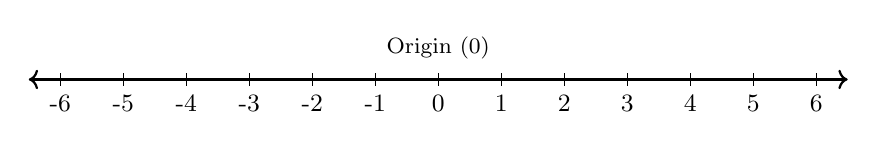
\begin{tikzpicture}[scale=0.8]
    \draw[<->, thick] (-6.5,0) -- (6.5,0);
    \foreach \x in {-6,-5,-4,-3,-2,-1,0,1,2,3,4,5,6}
        \draw (\x, 0.1) -- (\x, -0.1) node[below] {\small \x};
    \node at (0,0.5) {\footnotesize Origin (0)};
\end{tikzpicture}
\end{center}

\subsection*{Assessment Exercises: Identifying Integers}

\begin{solvingbox}{Question 1}
Identify integers: $A$ is 4 units left of 0, $B$ is 7 units right of 0. \\
Result: $A = \mathbf{-4}$, $B = \mathbf{+7}$ \hfill $A_1$
\end{solvingbox}

\begin{solvingbox}{Question 2}
A diver is \textbf{15 metres} below sea level. Write as an integer. \\
Result = \textbf{-15} \hfill $A_1$
\end{solvingbox}

\begin{solvingbox}{Question 3}
Arrange in \textbf{descending order}: $-10, 5, 0, -2, 8$. \\
Result = \textbf{8, 5, 0, -2, -10} \hfill $A_1$
\end{solvingbox}

\begin{solvingbox}{Question 4}
Which is greater: \textbf{-100} or \textbf{-5}? \\
On a number line, $-5$ is further to the right. \\
Result = \textbf{-5} \hfill $A_1$
\end{solvingbox}

\newpage

\subsection*{Operations on a Number Line}

\begin{solvingbox}{Question 1: $3 + (-5)$}
Start at 3, move 5 units to the \textbf{left}. \\
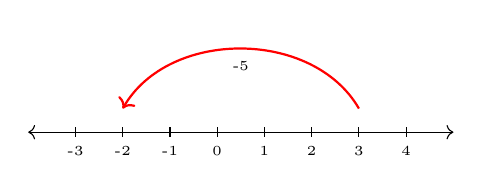
\begin{tikzpicture}[scale=0.6]
    \draw[<->] (-4,0) -- (5,0);
    \foreach \x in {-3,-2,-1,0,1,2,3,4} \draw (\x,0.1)--(\x,-0.1) node[below]{\tiny \x};
    \draw[->, red, thick] (3,0.5) to [out=120,in=60] (-2,0.5);
    \node at (0.5,1.4) {\tiny -5};
\end{tikzpicture} \\
Result = \textbf{-2} \hfill $A_1$
\end{solvingbox}

\begin{solvingbox}{Question 2: $-2 - 4$}
Start at -2, move 4 units to the \textbf{left}. \\
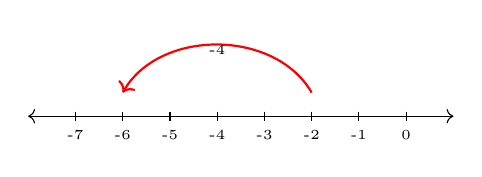
\begin{tikzpicture}[scale=0.6]
    \draw[<->] (-8,0) -- (1,0);
    \foreach \x in {-7,-6,-5,-4,-3,-2,-1,0} \draw (\x,0.1)--(\x,-0.1) node[below]{\tiny \x};
    \draw[->, red, thick] (-2,0.5) to [out=120,in=60] (-6,0.5);
    \node at (-4,1.4) {\tiny -4};
\end{tikzpicture} \\
Result = \textbf{-6} \hfill $A_1$
\end{solvingbox}

\begin{solvingbox}{Question 3: $1 - (-4)$}
Becomes $1 + 4$. Start at 1, move 4 units \textbf{right}. \\
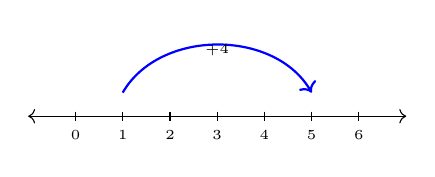
\begin{tikzpicture}[scale=0.6]
    \draw[<->] (-1,0) -- (7,0);
    \foreach \x in {0,1,2,3,4,5,6} \draw (\x,0.1)--(\x,-0.1) node[below]{\tiny \x};
    \draw[->, blue, thick] (1,0.5) to [out=60,in=120] (5,0.5);
    \node at (3,1.4) {\tiny +4};
\end{tikzpicture} \\
Result = \textbf{5} \hfill $A_1$
\end{solvingbox}

\subsection*{1.6.2 Combined Operations on Integers}

\begin{tcolorbox}[colback=lightgrey, colframe=primaryblue, title=\textbf{Concept Summary}, arc=5pt]
    \textbf{Sign Rules:}
    \begin{itemize}
        \item Same signs $\rightarrow$ Positive ($+ \times + = +$, $- \times - = +$)
        \item Different signs $\rightarrow$ Negative ($+ \times - = -$, $- \times + = -$)
    \end{itemize}
\end{tcolorbox}

\subsection*{Assessment Exercises (Mastery Level)}

\begin{solvingbox}{Question 1}
Evaluate: $-12 + (-4 \times -3)$ \\
Step 1: $-4 \times -3 = 12$. \hfill $M_1$ \\
Step 2: $-12 + 12 = 0$. \\
Result = \textbf{0} \hfill $A_1$
\end{solvingbox}

\begin{solvingbox}{Question 2}
Find: $15 \div (-3) \text{ of } 5$ \\
Step 1: $-3 \times 5 = -15$. \hfill $M_1$ \\
Step 2: $15 \div (-15) = -1$. \\
Result = \textbf{-1} \hfill $A_1$
\end{solvingbox}

\begin{solvingbox}{Question 3}
Work out: $(-8 + -2) \times (10 - 15)$ \\
Step 1: $(-10) \times (-5)$. \hfill $M_1$ \\
Step 2: $50$. \\
Result = \textbf{50} \hfill $A_1$
\end{solvingbox}

\begin{solvingbox}{Question 4}
Evaluate: $20 - [(-6 \text{ of } 2) + (-4)]$ \\
Step 1: $20 - [-12 - 4] = 20 - [-16]$. \hfill $M_1$ \\
Step 2: $20 + 16 = 36$. \\
Result = \textbf{36} \hfill $A_1$
\end{solvingbox}

\begin{solvingbox}{Question 5}
Calculate: $\frac{-48 \div 6}{-2 \times 2}$ \\
Step 1: Numerator $= -8$; Denominator $= -4$. \hfill $M_1$ \\
Step 2: $-8 \div -4 = 2$. \\
Result = \textbf{2} \hfill $A_1$
\end{solvingbox}
\begin{solvingbox}{Question 6}
Find the value of: $-5 \times (-3 + 7) \div (-2)$ \\
Step 1 (Bracket): $-3 + 7 = 4$ \hfill $M_1$ \\
Step 2 (Multiply): $-5 \times 4 = -20$ \hfill $M_1$ \\
Step 3 (Division): $-20 \div (-2) = \mathbf{10}$ \hfill $A_1$
\end{solvingbox}

\begin{solvingbox}{Question 7}
Evaluate: $100 \div (-5 \text{ of } -4) + (-3)$ \\
Step 1 (Of): $-5 \times -4 = 20$ \hfill $M_1$ \\
Step 2 (Division): $100 \div 20 = 5$ \hfill $M_1$ \\
Step 3 (Addition): $5 + (-3) = \mathbf{2}$ \hfill $A_1$
\end{solvingbox}

\begin{solvingbox}{Question 8}
Work out: $(-2)^3 + \sqrt{16} \div (-2)$ \\
Step 1 (Orders): $(-2)^3 = -8$ and $\sqrt{16} = 4$ \hfill $M_1$ \\
Step 2 (Division): $4 \div (-2) = -2$ \hfill $M_1$ \\
Step 3 (Addition): $-8 + (-2) = \mathbf{-10}$ \hfill $A_1$
\end{solvingbox}

\subsection*{1.6.3 Application of Integers to Real-Life Situations}

\begin{solvingbox}{Question 1 (Temperature Changes)}
At midnight in a certain town, the temperature was \textbf{$-5^\circ$C}. By noon the following day, the temperature had risen by \textbf{$12^\circ$C}. In the evening, it dropped by \textbf{$4^\circ$C}. Find the final temperature. \\
Initial: $-5$; Morning: $+12$; Evening: $-4$. \hfill $M_1$ \\
Working on line: $-5 \xrightarrow{+12} 7 \xrightarrow{-4} 3$. \\
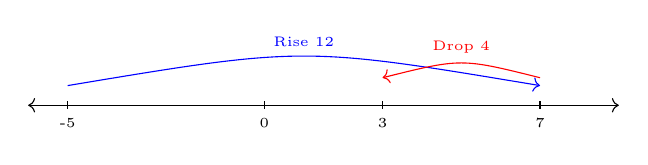
\begin{tikzpicture}[scale=0.5]
    \draw[<->] (-6,0) -- (9,0);
    \foreach \x in {-5,0,3,7} \draw (\x,0.1)--(\x,-0.1) node[below]{\tiny \x};
    \draw[->, blue] (-5,0.5) .. controls (1,1.5) .. (7,0.5) node[midway, above]{\tiny Rise 12};
    \draw[->, red] (7,0.7) .. controls (5,1.2) .. (3,0.7) node[midway, above]{\tiny Drop 4};
\end{tikzpicture} \\
Final Temperature = \textbf{$3^\circ$C} \hfill $A_1$
\end{solvingbox}

\begin{solvingbox}{Question 2 (Bank Account Balance)}
Mr. Mutua had a bank balance of \textbf{Sh. 4,500}. He withdrew \textbf{Sh. 6,000} to pay for supplies, creating an overdraft. Two days later, he deposited \textbf{Sh. 2,500}. What was his new balance? \\
Balance = $4500 - 6000 + 2500$ \hfill $M_1$ \\
$4500 - 6000 = -1500$ (Overdraft) \hfill $M_1$ \\
$-1500 + 2500 = +1000$ \\
Result = \textbf{Sh. 1,000} \hfill $A_1$
\end{solvingbox}

\begin{solvingbox}{Question 3 (Mountain and Sea Depth)}
A mountain peak is \textbf{4,800 metres} above sea level. Directly below it, there is a submarine trench \textbf{1,200 metres} deep. Calculate the vertical distance between the peak and the trench. \\
Peak = $+4800$; Trench = $-1200$. \hfill $M_1$ \\
Distance = $Peak - Trench = 4800 - (-1200)$ \hfill $M_1$ \\
$4800 + 1200 = \mathbf{6,000\text{ metres}}$ \hfill $A_1$
\end{solvingbox}

\begin{solvingbox}{Question 4 (Elevator Movement)}
An elevator in a tall building is on the \textbf{15th floor}. it goes down \textbf{18 floors} to a basement parking level and then goes up \textbf{7 floors}. On which floor is the elevator now? \\
Current floor = $15 - 18 + 7$ \hfill $M_1$ \\
$15 - 18 = -3$ (3rd Basement) \hfill $M_1$ \\
$-3 + 7 = 4$. \\
Result = \textbf{4th Floor} \hfill $A_1$
\end{solvingbox}

\begin{solvingbox}{Question 5 (Time Zones)}
A football match starts in London at \textbf{20:00 hours}. The time in Mombasa is \textbf{3 hours ahead} of London, while the time in New York is \textbf{5 hours behind} London. Find the time in Mombasa and New York. \\
London = 0; Mombasa = $+3$; New York = $-5$. \hfill $M_1$ \\
Mombasa: $20:00 + 3 = \mathbf{23:00\text{ hours}}$ \hfill $A_1$ \\
New York: $20:00 - 5 = \mathbf{15:00\text{ hours}}$ \hfill $A_1$
\end{solvingbox}

\begin{solvingbox}{Question 6 (Business Profit and Loss)}
A trader made a profit of \textbf{Sh. 1,200} on Monday, a loss of \textbf{Sh. 850} on Tuesday, and a loss of \textbf{Sh. 500} on Wednesday. Calculate the net profit or loss for the three days. \\
Total = $+1200 - 850 - 500$ \hfill $M_1$ \\
$1200 - 850 = 350$ \\
$350 - 500 = -150$ \hfill $M_1$ \\
Result = \textbf{Loss of Sh. 150} \hfill $A_1$
\end{solvingbox}

\begin{solvingbox}{Question 7 (Scoring System)}
In a quiz, students get \textbf{+5 points} for every correct answer and \textbf{$-2$ points} for every wrong answer. If Mary got 12 questions correct and 8 questions wrong, what was her total score? \\
Correct: $12 \times 5 = 60$ \hfill $M_1$ \\
Wrong: $8 \times -2 = -16$ \hfill $M_1$ \\
Total = $60 + (-16) = \mathbf{44\text{ points}}$ \hfill $A_1$
\end{solvingbox}

\begin{solvingbox}{Question 8 (Diving and Flight)}
A bird is flying at \textbf{25 metres} above a lake. A fish is swimming \textbf{3 metres} below the surface. A kingfisher dives from the bird's height to catch the fish. How many metres did the kingfisher dive? \\
Start = $+25$; End = $-3$. \hfill $M_1$ \\
Dive Distance = $25 - (-3) = 25 + 3$ \hfill $M_1$ \\
Result = \textbf{28 metres} \hfill $A_1$
\end{solvingbox}

\begin{solvingbox}{Question 9 (Temperature in a Freezer)}
The temperature of a freezer is set at \textbf{$-18^\circ$C}. During a power outage, the temperature rose by \textbf{$2^\circ$C every hour}. What was the temperature after \textbf{5 hours}? \\
Initial = $-18$. Rise = $5 \times 2 = +10$. \hfill $M_1$ \\
New Temp = $-18 + 10 = \mathbf{-8^\circ C}$ \hfill $A_1$
\end{solvingbox}

\begin{solvingbox}{Question 10 (Historical Timeline)}
A famous scholar was born in the year \textbf{45 BC} and died in the year \textbf{15 AD}. How old was the scholar when he died? \\
Birth = $-45$; Death = $+15$. \hfill $M_1$ \\
Age = $15 - (-45) = 15 + 45$. \hfill $M_1$ \\
Result = \textbf{60 years} \hfill $A_1$
\end{solvingbox}

\begin{solvingbox}{Question 11 (Submarine Maneuvers)}
A submarine at \textbf{250 m} below sea level descends a further \textbf{150 m} and then ascends \textbf{80 m}. Find its final depth relative to sea level. \\
Depth = $-250 - 150 + 80$ \hfill $M_1$ \\
$-400 + 80 = -320$ \hfill $M_1$ \\
Result = \textbf{320 m below sea level} \hfill $A_1$
\end{solvingbox}

\begin{solvingbox}{Question 12 (Water Tank Levels)}
A borehole pump fills a tank at a rate that increases the water level by \textbf{0.4 m per hour}, while usage by cattle decreases it by \textbf{0.6 m per hour}. If the level was at \textbf{2.5 m} initially, what is the level after \textbf{10 hours} of simultaneous pumping and usage? \\
Change per hour = $+0.4 - 0.6 = -0.2\text{ m}$ \hfill $M_1$ \\
Total change = $-0.2 \times 10 = -2\text{ m}$ \hfill $M_1$ \\
Final level = $2.5 - 2 = \mathbf{0.5\text{ m}}$ \hfill $A_1$
\end{solvingbox}

\section*{1.7 CUBES AND CUBE ROOTS}

\subsection*{1.7.1 Cubes of Whole Numbers, Fractions, and Decimals}

\begin{tcolorbox}[colback=lightgrey, colframe=primaryblue, title=\textbf{Concept Summary}, arc=5pt]
    The \textbf{cube} of a number is the result of multiplying the number by itself three times ($n \times n \times n$).
    \begin{itemize}
        \item \textbf{Whole Numbers:} $n^3 = n \times n \times n$.
        \item \textbf{Fractions:} $(\frac{a}{b})^3 = \frac{a^3}{b^3}$.
        \item \textbf{Decimals:} Cube as whole numbers, then \textbf{triple} the number of decimal places.
    \end{itemize}
\end{tcolorbox}

\subsection*{Assessment Exercises (Mastery Level)}

\begin{solvingbox}{Question 1}
Find the cube of \textbf{6}. \\
$6^3 = 6 \times 6 \times 6$ \hfill $M_1$ \\
$36 \times 6 = \mathbf{216}$ \hfill $A_1$
\end{solvingbox}

\begin{solvingbox}{Question 2}
Calculate the cube of \textbf{12}. \\
$12^3 = 12 \times 12 \times 12$ \hfill $M_1$ \\
$144 \times 12 = \mathbf{1,728}$ \hfill $A_1$
\end{solvingbox}

\begin{solvingbox}{Question 3}
Work out the value of \textbf{$0.3^3$}. \\
$3^3 = 27$ \hfill $M_1$ \\
One decimal place becomes $1 \times 3 = 3$ decimal places. \\
Result = \textbf{0.027} \hfill $A_1$
\end{solvingbox}

\begin{solvingbox}{Question 4}
What is the cube of \textbf{1.1}? \\
$11^3 = 11 \times 11 \times 11 = 1331$ \hfill $M_1$ \\
Result = \textbf{1.331} \hfill $A_1$
\end{solvingbox}

\begin{solvingbox}{Question 5}
Evaluate $(\frac{2}{5})^3$. \\
$(\frac{2}{5})^3 = \frac{2 \times 2 \times 2}{5 \times 5 \times 5}$ \hfill $M_1$ \\
Result = $\mathbf{\frac{8}{125}}$ \hfill $A_1$
\end{solvingbox}

\begin{solvingbox}{Question 6}
Find the cube of the mixed fraction $\mathbf{1\frac{1}{2}}$. \\
$1\frac{1}{2} = \frac{3}{2}$ \hfill $M_1$ \\
$(\frac{3}{2})^3 = \frac{27}{8} = \mathbf{3\frac{3}{8}}$ \hfill $A_1$
\end{solvingbox}

\begin{solvingbox}{Question 7}
A cubic water tank has a side of \textbf{2 metres}. Calculate its volume in cubic metres. \\
Volume = $Side^3 = 2 \times 2 \times 2$ \hfill $M_1$ \\
Result = $\mathbf{8\text{ m}^3}$ \hfill $A_1$
\end{solvingbox}

\begin{solvingbox}{Question 8}
What is the cube of \textbf{0.04}? \\
$4^3 = 64$ \hfill $M_1$ \\
Two decimal places become $2 \times 3 = 6$ decimal places. \\
Result = \textbf{0.000064} \hfill $A_1$
\end{solvingbox}

\begin{solvingbox}{Question 9}
Find the volume of a cube whose side is \textbf{0.5 cm}. \\
$0.5^3 = 5^3 \times 10^{-3}$ \hfill $M_1$ \\
$125 \times 0.001 = \mathbf{0.125\text{ cm}^3}$ \hfill $A_1$
\end{solvingbox}

\subsection*{1.7.2 Cubes of Numbers Using Mathematical Tables}

\begin{tcolorbox}[colback=lightgrey, colframe=primaryblue, title=\textbf{Step-by-Step Table Usage}, arc=5pt]
    To find the cube of a number $x$ using tables:
    \begin{enumerate}
        \item \textbf{Standard Form:} Ensure the number is between 1 and 10 (e.g., $x = a \times 10^n$).
        \item \textbf{Row:} Find the first two digits of $a$ in the vertical column.
        \item \textbf{Column:} Move horizontally to the column of the third digit.
        \item \textbf{Mean Difference:} Add the value from the fourth digit's column.
        \item \textbf{Power Adjustment:} Multiply by $10^{3n}$.
    \end{enumerate}
\end{tcolorbox}

\begin{solvingbox}{Question 1 (Direct)}
Find the cube of \textbf{4.28} using tables. \\
1. Row 4.2, Column 8 $\rightarrow$ 78.395 \hfill $M_1$ \\
Result = \textbf{78.395} \hfill $A_1$
\end{solvingbox}

\begin{solvingbox}{Question 2 (Direct)}
Find $8.156^3$ using tables. \\
1. Row 8.1, Column 5 $\rightarrow$ 540.8 \hfill $M_1$ \\
2. Mean difference for 6 $\rightarrow$ 1.2 \hfill $M_1$ \\
3. $540.8 + 1.2 = \mathbf{542.0}$ \hfill $A_1$
\end{solvingbox}

\begin{solvingbox}{Question 3 (Direct)}
Evaluate $0.234^3$ using tables. \\
1. $2.34 \times 10^{-1} \rightarrow (2.34)^3 \times 10^{-3}$ \hfill $M_1$ \\
2. $(2.34)^3$ from table $\rightarrow$ 12.81 \hfill $M_1$ \\
3. $12.81 \times 10^{-3} = \mathbf{0.01281}$ \hfill $A_1$
\end{solvingbox}

\begin{solvingbox}{Question 4 (Direct)}
Use tables to find $45.2^3$. \\
1. $4.52 \times 10^1 \rightarrow (4.52)^3 \times 10^3$ \hfill $M_1$ \\
2. $(4.52)^3$ from table $\rightarrow$ 92.35 \hfill $M_1$ \\
3. $92.35 \times 1,000 = \mathbf{92,350}$ \hfill $A_1$
\end{solvingbox}

\begin{solvingbox}{Question 5 (Direct)}
Find $1.093^3$ using tables. \\
1. Row 1.0, Col 9 $\rightarrow$ 1.295 \hfill $M_1$ \\
2. Mean diff for 3 $\rightarrow$ 0.011 \hfill $M_1$ \\
Result = \textbf{1.306} \hfill $A_1$
\end{solvingbox}

\begin{solvingbox}{Question 6 (Application)}
A cubic container has a side length of \textbf{3.55 cm}. Find its volume using tables. \\
1. Row 3.5, Col 5 $\rightarrow$ 44.739 \hfill $M_1$ \\
Result = $\mathbf{44.739\text{ cm}^3}$ \hfill $A_1$
\end{solvingbox}

\begin{solvingbox}{Question 7 (Application)}
A metal block is a cube with a side of \textbf{0.62 m}. Calculate its volume using tables. \\
1. $6.2 \times 10^{-1} \rightarrow (6.2)^3 \times 10^{-3}$ \hfill $M_1$ \\
2. $6.2^3$ from table $\rightarrow$ 238.3 \hfill $M_1$ \\
3. $238.3 \div 1000 = \mathbf{0.2383\text{ m}^3}$ \hfill $A_1$
\end{solvingbox}

\begin{solvingbox}{Question 8 (Application)}
Find the capacity of a cubic tank of side \textbf{1.84 metres}. \\
1. Row 1.8, Col 4 $\rightarrow$ 6.230 \hfill $M_1$ \\
Result = $\mathbf{6.23\text{ m}^3}$ \hfill $A_1$
\end{solvingbox}

\begin{solvingbox}{Question 9 (Application)}
The side of a small dice is \textbf{15 mm}. Find its volume in $\text{mm}^3$ using tables. \\
1. $1.5 \times 10^1 \rightarrow 1.5^3 \times 10^3$ \hfill $M_1$ \\
2. $1.5^3 = 3.375$ \hfill $M_1$ \\
3. $3.375 \times 1000 = \mathbf{3,375\text{ mm}^3}$ \hfill $A_1$
\end{solvingbox}

\begin{solvingbox}{Question 10 (Application)}
Evaluate $x^3$ if $x = 0.0982$. \\
1. $9.82 \times 10^{-2} \rightarrow 9.82^3 \times 10^{-6}$ \hfill $M_1$ \\
2. $9.82^3 = 947.2$ \hfill $M_1$ \\
3. $947.2 \times 10^{-6} = \mathbf{0.0009472}$ \hfill $A_1$
\end{solvingbox}

\begin{solvingbox}{Question 11 (Application)}
A cubic room has a length of \textbf{2.715 m}. Find the volume of air it contains. \\
1. Row 2.7, Col 1 $\rightarrow$ 19.903 \hfill $M_1$ \\
2. Mean diff for 5 $\rightarrow$ 0.110 \hfill $M_1$ \\
3. $19.903 + 0.110 = \mathbf{20.013\text{ m}^3}$ \hfill $A_1$
\end{solvingbox}

\begin{solvingbox}{Question 12 (Application)}
What is the cube of \textbf{7.409}? \\
1. Row 7.4, Col 0 $\rightarrow$ 405.2 \hfill $M_1$ \\
2. Mean diff for 9 $\rightarrow$ 1.5 \hfill $M_1$ \\
Result = \textbf{406.7} \hfill $A_1$
\end{solvingbox}

\begin{solvingbox}{Question 13 (Application)}
If a side of a cube is \textbf{5.004 cm}, find its volume. \\
1. Row 5.0, Col 0 $\rightarrow$ 125.0 \hfill $M_1$ \\
2. Mean diff for 4 $\rightarrow$ 0.3 \hfill $M_1$ \\
Result = \textbf{125.3 $\text{cm}^3$} \hfill $A_1$
\end{solvingbox}

\subsection*{1.7.3 Cube Roots Using Prime Factorization}

\begin{tcolorbox}[colback=lightgrey, colframe=primaryblue, title=\textbf{Concept Summary}, arc=5pt]
    To find the cube root ($\sqrt[3]{x}$) of a number using prime factors:
    \begin{enumerate}
        \item Factorize the number into its prime components using a factor tree.
        \item Group the prime factors into \textbf{triplets} (sets of three identical factors).
        \item Pick one factor from each triplet and multiply them to get the cube root.
    \end{enumerate}
\end{tcolorbox}
\subsection*{Assessment Exercises (Mastery Level)}

\begin{solvingbox}{Question 1}
Find the cube root of \textbf{216} using prime factorization. \\
\textbf{Factor Tree:} \\
$216 \rightarrow 2 \times 108 \rightarrow 2^2 \times 54 \rightarrow 2^3 \times 27 \rightarrow 2^3 \times 3 \times 9 \rightarrow 2^3 \times 3^3$ \hfill $M_1$ \\
$216 = (2 \times 2 \times 2) \times (3 \times 3 \times 3)$ \\
Grouping into triplets: $(2) \times (3)$ \\
$\sqrt[3]{216} = 2 \times 3 = \mathbf{6}$ \hfill $A_1$
\end{solvingbox}

\begin{solvingbox}{Question 2}
Calculate $\sqrt[3]{512}$ using the factor method. \\
\textbf{Factor Tree:} \\
$512 \rightarrow 2 \times 256 \rightarrow 2^2 \times 128 \rightarrow 2^3 \times 64 \rightarrow 2^4 \times 32 \rightarrow 2^5 \times 16 \rightarrow 2^6 \times 8 \rightarrow 2^9$ \hfill $M_1$ \\
$512 = (2 \times 2 \times 2) \times (2 \times 2 \times 2) \times (2 \times 2 \times 2)$ \\
$\sqrt[3]{512} = 2 \times 2 \times 2 = \mathbf{8}$ \hfill $A_1$
\end{solvingbox}

\begin{solvingbox}{Question 3}
Work out the cube root of \textbf{1,000}. \\
\textbf{Factor Tree:} \\
$1000 \rightarrow 10 \times 100 \rightarrow (2 \times 5) \times (10 \times 10) \rightarrow (2 \times 5) \times (2 \times 5) \times (2 \times 5)$ \hfill $M_1$ \\
$1000 = 2^3 \times 5^3$ \\
$\sqrt[3]{1000} = 2 \times 5 = \mathbf{10}$ \hfill $A_1$
\end{solvingbox}

\begin{solvingbox}{Question 4}
Find the side length of a cubic block whose volume is \textbf{3,375 $\text{cm}^3$}. \\
$3375 \rightarrow 3 \times 1125 \rightarrow 3^2 \times 375 \rightarrow 3^3 \times 125 \rightarrow 3^3 \times 5^3$ \hfill $M_1$ \\
Triplets: $(3 \times 3 \times 3)$ and $(5 \times 5 \times 5)$ \\
$\sqrt[3]{3375} = 3 \times 5 = \mathbf{15\text{ cm}}$ \hfill $A_1$
\end{solvingbox}

\begin{solvingbox}{Question 5}
What is the cube root of \textbf{8,000}? \\
$8000 = 8 \times 1000 = 2^3 \times 10^3 = 2^3 \times (2 \times 5)^3 = 2^6 \times 5^3$ \hfill $M_1$ \\
$\sqrt[3]{8000} = 2^2 \times 5 = 4 \times 5 = \mathbf{20}$ \hfill $A_1$
\end{solvingbox}

\begin{solvingbox}{Question 6}
Evaluate $\sqrt[3]{1728}$ using prime factorization. \\
$1728 \rightarrow 2 \times 864 \rightarrow 2^2 \times 432 \rightarrow 2^3 \times 216 \rightarrow 2^3 \times 6^3$ \\
$1728 = 2^3 \times (2 \times 3)^3 = 2^6 \times 3^3$ \hfill $M_1$ \\
$\sqrt[3]{1728} = 2^2 \times 3 = 4 \times 3 = \mathbf{12}$ \hfill $A_1$
\end{solvingbox}

\begin{solvingbox}{Question 7}
A tank holds \textbf{27,000 litres} of water. If the tank is a cube, find its side in metres ($1000\text{ litres} = 1\text{ m}^3$). \\
Volume = $27\text{ m}^3$ \hfill $M_1$ \\
$27 \rightarrow 3 \times 9 \rightarrow 3 \times 3 \times 3$ \\
$\sqrt[3]{27} = \mathbf{3\text{ metres}}$ \hfill $A_1$
\end{solvingbox}

\begin{solvingbox}{Question 8}
Find $\sqrt[3]{9261}$ using prime factors. \\
$9261 \rightarrow 3 \times 3087 \rightarrow 3^2 \times 1029 \rightarrow 3^3 \times 343 \rightarrow 3^3 \times 7^3$ \hfill $M_1$ \\
$\sqrt[3]{9261} = 3 \times 7 = \mathbf{21}$ \hfill $A_1$
\end{solvingbox}

\subsection*{1.7.4 Cube Roots Using the Table of Cubes (Inverse Method)}

\begin{tcolorbox}[colback=lightgrey, colframe=primaryblue, title=\textbf{Methodology: The Inverse Look-up}, arc=5pt]
    Since four-figure tables typically provide a \textbf{Table of Cubes} ($x^3$) but not a dedicated cube root table, we use the "Inverse Method":
    \begin{enumerate}
        \item \textbf{Prepare the Number:} Express the number in the form $a \times 10^n$, where $n$ is a \textbf{multiple of 3} (e.g., $10^0, 10^3, 10^6, 10^{-3}$). This ensures $a$ is a value found in the body of the Cube Table ($1.000$ to $999.9$).
        \item \textbf{The Search:} Look for the value $a$ \textbf{inside the body} of the table (the main grid).
        \item \textbf{The Read:} 
            \begin{itemize}
                \item The first two digits of the root are in the \textbf{left-hand column ($x$)}.
                \item The third digit is in the \textbf{top header row}.
                \item The fourth digit is found by checking the \textbf{mean differences} row to find the closest match to your remaining remainder.
            \end{itemize}
        \item \textbf{Final Step:} Multiply the value found by $10^{n/3}$.
    \end{enumerate}
\end{tcolorbox}

\subsection*{Assessment Exercises (Mastery Level)}

\begin{solvingbox}{Question 1 (Direct)}
Find $\sqrt[3]{115.8}$ using the Table of Cubes. \\
1. Search the body for the value closest to \textbf{115.8}. \hfill $M_1$ \\
2. In row \textbf{4.8}, column \textbf{7}, the value is $112.2$. Column \textbf{8} is $114.5$. \\
3. In row \textbf{4.8}, column \textbf{9}, the value is $117.2$. \\
4. The closest value is $115.8$, which corresponds to $x = \mathbf{4.875}$ (approx). \hfill $A_1$
\end{solvingbox}

\begin{solvingbox}{Question 2 (Direct)}
Find the cube root of \textbf{40.5} using the table. \\
1. Look for \textbf{40.5} in the grid. \hfill $M_1$ \\
2. Row \textbf{3.4}, column \textbf{3} gives $39.30$. Column \textbf{4} gives $40.45$. \\
3. $40.45$ is almost exactly $40.5$. \\
Result = \textbf{3.434} \hfill $A_1$
\end{solvingbox}

\begin{solvingbox}{Question 3 (Direct)}
Work out $\sqrt[3]{729,000}$ using the Table of Cubes. \\
1. Standard form: $\sqrt[3]{729 \times 10^3} = \sqrt[3]{729} \times 10$. \hfill $M_1$ \\
2. Search body for \textbf{729}. It matches row \textbf{9.0}, column \textbf{0} exactly. \hfill $M_1$ \\
3. $9.0 \times 10 = \mathbf{90}$ \hfill $A_1$
\end{solvingbox}

\begin{solvingbox}{Question 4 (Direct)}
Evaluate $\sqrt[3]{0.005832}$ using the inverse table method. \\
1. Standard form: $\sqrt[3]{5.832 \times 10^{-3}} = \sqrt[3]{5.832} \times 0.1$. \hfill $M_1$ \\
2. Search body for \textbf{5.832}. It matches row \textbf{1.8}, column \textbf{0}. \hfill $M_1$ \\
3. $1.8 \times 0.1 = \mathbf{0.18}$ \hfill $A_1$
\end{solvingbox}

\begin{solvingbox}{Question 5 (Direct)}
Find the cube root of \textbf{250} using the table. \\
1. Search body for \textbf{250}. \hfill $M_1$ \\
2. Row \textbf{6.3}, column \textbf{0} is $250.0$. \hfill $M_1$ \\
Result = \textbf{6.3} \hfill $A_1$
\end{solvingbox}

\begin{solvingbox}{Question 6 (Word Problem)}
A cubic container has a volume of \textbf{19.683 $\text{cm}^3$}. Find its side using tables. \\
1. Search body for \textbf{19.683}. \hfill $M_1$ \\
2. It matches row \textbf{2.7}, column \textbf{0}. \hfill $M_1$ \\
Result = \textbf{2.7 cm} \hfill $A_1$
\end{solvingbox}

\begin{solvingbox}{Question 7 (Word Problem)}
Calculate the radius of a sphere with a volume of \textbf{38.808 $\text{cm}^3$} (Take $\pi = \frac{22}{7}$). \\
$V = \frac{4}{3}\pi r^3 \implies 38.808 = \frac{4}{3} \cdot \frac{22}{7} \cdot r^3 \implies r^3 = 9.261$. \hfill $M_1$ \\
1. Search body for \textbf{9.261}. Matches row \textbf{2.1}, column \textbf{0}. \hfill $M_1$ \\
Result = \textbf{2.1 cm} \hfill $A_1$
\end{solvingbox}

\begin{solvingbox}{Question 8 (Word Problem)}
A water tank in the shape of a cube has a capacity of \textbf{3,375 litres}. Find its side in metres. \\
$3375\text{ L} = 3.375\text{ m}^3$. \hfill $M_1$ \\
1. Search body for \textbf{3.375}. Matches row \textbf{1.5}, column \textbf{0}. \hfill $M_1$ \\
Result = \textbf{1.5 m} \hfill $A_1$
\end{solvingbox}

\begin{solvingbox}{Question 9 (Word Problem)}
If $x^3 = 0.512$, find the value of $x$ using the table. \\
1. $\sqrt[3]{512 \times 10^{-3}}$. Search body for \textbf{512}. \hfill $M_1$ \\
2. Matches row \textbf{8.0}, column \textbf{0}. \hfill $M_1$ \\
3. $8.0 \times 10^{-1} = \mathbf{0.8}$ \hfill $A_1$
\end{solvingbox}

\begin{solvingbox}{Question 10 (Word Problem)}
Find the length of a side of a cube whose volume is \textbf{150 $\text{cm}^3$}. \\
1. Search body for \textbf{150}. \hfill $M_1$ \\
2. Row \textbf{5.3}, column \textbf{1} is $148.9$. Column \textbf{2} is $149.7$. \hfill $M_1$ \\
Result = \textbf{5.314 cm} (Approx) \hfill $A_1$
\end{solvingbox}

\begin{solvingbox}{Question 11 (Word Problem)}
A cube of sugar has a volume of \textbf{4,096 $\text{mm}^3$}. Find its side length. \\
1. $\sqrt[3]{4.096 \times 10^3}$. Search body for \textbf{4.096}. \hfill $M_1$ \\
2. Matches row \textbf{1.6}, column \textbf{0}. \hfill $M_1$ \\
3. $1.6 \times 10 = \mathbf{16\text{ mm}}$ \hfill $A_1$
\end{solvingbox}

\begin{solvingbox}{Question 12 (Word Problem)}
A cubic wooden block has a mass of \textbf{2.7 kg} and a density of \textbf{$1\text{ g/cm}^3$}. Find its side. \\
$V = \frac{m}{\rho} = \frac{2700\text{ g}}{1\text{ g/cm}^3} = 2700\text{ cm}^3$. \hfill $M_1$ \\
1. $\sqrt[3]{2.7 \times 10^3}$. Search body for \textbf{2.7}. \hfill $M_1$ \\
2. Matches row \textbf{1.3}, column \textbf{9} ($\approx 2.686$). \\
Result = \textbf{13.92 cm} \hfill $A_1$
\end{solvingbox}

\newpage

\subsection*{1.7.5 Real-Life Applications of Cubes and Cube Roots}

\begin{solvingbox}{Question 1}
A cylindrical metal rod has a radius of \textbf{4 cm} and a height of \textbf{18 cm}. It is melted down and recast into a cube. Calculate the side of the cube formed (Take $\pi = 3.142$). \\
$V_{\text{cylinder}} = \pi r^2 h = 3.142 \times 4^2 \times 18$. \hfill $M_1$ \\
$V = 3.142 \times 16 \times 18 = 904.896\text{ cm}^3$. \hfill $M_1$ \\
Side of cube $s = \sqrt[3]{904.896}$. \\
From table: Row 9.6, Col 7 gives 904.2. \hfill $M_1$ \\
Result = \textbf{9.67 cm} \hfill $A_1$
\end{solvingbox}

\begin{solvingbox}{Question 2}
Three small cubic lead blocks with sides \textbf{3 cm, 4 cm, and 5 cm} are melted together to form one large cube. Find the side length of the new cube. \\
Total Volume $= 3^3 + 4^3 + 5^3 = 27 + 64 + 125$. \hfill $M_1$ \\
$V = 216\text{ cm}^3$. \hfill $M_1$ \\
Side $= \sqrt[3]{216} = \mathbf{6\text{ cm}}$ \hfill $A_1$
\end{solvingbox}

\begin{solvingbox}{Question 3}
A cubic water tank holds \textbf{15,625 litres} of water. If the water is used to fill 125 smaller identical cubic containers, what is the side length of each small container in cm? \\
Volume per small cube $= 15625 \div 125 = 125\text{ litres}$. \hfill $M_1$ \\
$125\text{ litres} = 125,000\text{ cm}^3$. \hfill $M_1$ \\
Side $= \sqrt[3]{125,000} = 50\text{ cm}$. \hfill $A_1$
\end{solvingbox}

\begin{solvingbox}{Question 4}
The volume of a sphere is \textbf{310.4 $\text{cm}^3$}. If this sphere is reshaped into a cube, find the length of the side of the cube correct to 2 decimal places. \\
$V_{\text{cube}} = V_{\text{sphere}} = 310.4$. \hfill $M_1$ \\
Side $= \sqrt[3]{310.4}$. From table: Row 6.7, Col 7 is 303; Col 8 is 310. \hfill $M_1$ \\
Result = \textbf{6.77 cm} \hfill $A_1$
\end{solvingbox}

\begin{solvingbox}{Question 5}
A rectangular block of ice measuring \textbf{16 cm by 8 cm by 4 cm} melts. If the water is frozen into a single cube, find the side of that cube. \\
$V = 16 \times 8 \times 4 = 512\text{ cm}^3$. \hfill $M_1$ \\
Side $= \sqrt[3]{512}$. \hfill $M_1$ \\
Result = \textbf{8 cm} \hfill $A_1$
\end{solvingbox}

\begin{solvingbox}{Question 6}
A solid cylinder with radius \textbf{7 cm} and height \textbf{10 cm} is melted to make small cubes of side \textbf{2 cm}. How many complete cubes can be made? (Take $\pi = \frac{22}{7}$). \\
$V_{\text{cyl}} = \frac{22}{7} \times 7^2 \times 10 = 1540\text{ cm}^3$. \hfill $M_1$ \\
$V_{\text{cube}} = 2^3 = 8\text{ cm}^3$. \hfill $M_1$ \\
Number of cubes $= 1540 \div 8 = 192.5$. \hfill $M_1$ \\
Result = \textbf{192 cubes} \hfill $A_1$
\end{solvingbox}

\begin{solvingbox}{Question 7}
The ratio of the volumes of two cubes is \textbf{8:27}. If the side of the smaller cube is \textbf{10 cm}, find the side of the larger cube. \\
Ratio of sides $= \sqrt[3]{8} : \sqrt[3]{27} = 2:3$. \hfill $M_1$ \\
If $2 \to 10\text{ cm}$, then $1 \to 5\text{ cm}$. \\
$3 \times 5 = \mathbf{15\text{ cm}}$ \hfill $A_1$
\end{solvingbox}

\begin{solvingbox}{Question 8}
A cubic tank has a capacity of \textbf{1 hectare-metre} (volume of water 1m deep over 1 hectare). Calculate the side of this cube in metres ($1\text{ ha} = 10,000\text{ m}^2$). \\
$V = 10,000 \times 1 = 10,000\text{ m}^3$. \hfill $M_1$ \\
Side $= \sqrt[3]{10,000} = \sqrt[3]{10 \times 10^3}$. \hfill $M_1$ \\
From table: $\sqrt[3]{10} \approx 2.154$. \\
$2.154 \times 10 = \mathbf{21.54\text{ m}}$ \hfill $A_1$
\end{solvingbox}

\begin{solvingbox}{Question 9}
A copper wire of length \textbf{100 m} and diameter \textbf{2 cm} is melted and cast into a cube. Find the side of the cube. \\
$r = 1\text{ cm}, h = 10,000\text{ cm}$. \hfill $M_1$ \\
$V = \pi \times 1^2 \times 10,000 = 31,420\text{ cm}^3$. \hfill $M_1$ \\
Side $= \sqrt[3]{31,420} = \sqrt[3]{31.42 \times 10^3}$. \hfill $M_1$ \\
Result = \textbf{31.56 cm} \hfill $A_1$
\end{solvingbox}

\begin{solvingbox}{Question 10}
If the side of a cube is doubled, by what factor does its volume increase? \\
Let original side be $s$, then $V_1 = s^3$. \hfill $M_1$ \\
New side $= 2s$, then $V_2 = (2s)^3 = 8s^3$. \hfill $M_1$ \\
Result = \textbf{Factor of 8} \hfill $A_1$
\end{solvingbox}

\section*{1.8 RATES, RATIO, PROPORTIONS AND PERCENTAGES}

\subsection*{1.8.1 (a) Rate of Work (Grades 7--9 Integration)}

\begin{tcolorbox}[colback=lightgrey, colframe=primaryblue, title=\textbf{Teacher's Key Concept: The Reciprocal Rule}, arc=5pt]
    To solve work rate problems:
    \begin{enumerate}
        \item Determine the fraction of work done in \textbf{one unit of time} (e.g., 1 hour or 1 day). 
        \item If person A takes $x$ days and person B takes $y$ days, their combined rate per day is $\frac{1}{x} + \frac{1}{y}$.
        \item For pipes, \textbf{inlet} pipes have a positive rate ($+$) and \textbf{outlet/drain} pipes have a negative rate ($-$).
    \end{enumerate}
\end{tcolorbox}

\subsection*{Assessment Exercises: Rate of Work}

\begin{solvingbox}{Question 1}
Tap A can fill a tank in \textbf{3 hours}, while Tap B can fill the same tank in \textbf{6 hours}. If both taps are opened at the same time, how long will they take to fill the tank? \\
Rate of A $= \frac{1}{3}$ per hour; Rate of B $= \frac{1}{6}$ per hour. \hfill $M_1$ \\
Combined rate $= \frac{1}{3} + \frac{1}{6} = \frac{2+1}{6} = \frac{3}{6} = \frac{1}{2}$ tank/hr. \hfill $M_1$ \\
Time taken $= 1 \div \frac{1}{2} = \mathbf{2\text{ hours}}$ \hfill $A_1$
\end{solvingbox}

\begin{solvingbox}{Question 2}
Three workers, Musau, Onyando, and Beth, can complete a piece of work in \textbf{10, 15, and 30 days} respectively. How long would it take them to complete the work if they all work together? \\
Combined rate $= \frac{1}{10} + \frac{1}{15} + \frac{1}{30}$ \hfill $M_1$ \\
$\text{L.C.M} = 30 \implies \frac{3+2+1}{30} = \frac{6}{30} = \frac{1}{5}$ work/day. \hfill $M_1$ \\
Time taken $= 1 \div \frac{1}{5} = \mathbf{5\text{ days}}$ \hfill $A_1$
\end{solvingbox}

\begin{solvingbox}{Question 3}
A swimming pool has two inlet pipes that can fill it in \textbf{4 hours} and \textbf{12 hours} respectively. An outlet pipe can empty the full pool in \textbf{6 hours}. If all three pipes are opened together, how long will it take to fill the pool? \\
Net rate $= \frac{1}{4} + \frac{1}{12} - \frac{1}{6}$ \hfill $M_1$ \\
$\frac{3+1-2}{12} = \frac{2}{12} = \frac{1}{6}$ pool/hr. \hfill $M_1$ \\
Time taken $= \mathbf{6\text{ hours}}$ \hfill $A_1$
\end{solvingbox}

\begin{solvingbox}{Question 4}
Peter can type a document in \textbf{40 minutes}. After working for \textbf{10 minutes}, he is joined by Jane, and they finish the document in another \textbf{12 minutes}. How long would Jane have taken to type the document alone? \\
Peter's rate $= \frac{1}{40}$. In 10 min, he did $10 \times \frac{1}{40} = \frac{1}{4}$ of the work. \hfill $M_1$ \\
Remaining work $= 1 - \frac{1}{4} = \frac{3}{4}$. \hfill $M_1$ \\
In 12 min, combined work $= \frac{3}{4} \implies$ Combined rate $= \frac{3}{4} \div 12 = \frac{1}{16}$. \\
Jane's rate $= \frac{1}{16} - \frac{1}{40} = \frac{5-2}{80} = \frac{3}{80}$. \\
Jane's time $= 1 \div \frac{3}{80} = 26 \frac{2}{3} \text{ minutes or } \mathbf{26\text{ min } 40\text{ sec}}$ \hfill $A_1$
\end{solvingbox}

\begin{solvingbox}{Question 5}
8 men can weed a farm in \textbf{6 days}. If the farm must be weeded in \textbf{4 days}, how many \textbf{extra} men should be hired, assuming they work at the same rate? \\
Total man-days $= 8 \times 6 = 48$ man-days. \hfill $M_1$ \\
Men needed for 4 days $= 48 \div 4 = 12$ men. \hfill $M_1$ \\
Extra men $= 12 - 8 = \mathbf{4\text{ extra men}}$ \hfill $A_1$
\end{solvingbox}

\begin{solvingbox}{Question 6}
A contractor estimated that \textbf{20 workers} could build a wall in \textbf{15 days}. After working for \textbf{3 days}, \textbf{5 workers} fell ill and left. How many \textbf{more} days will the remaining workers take to finish the wall? \\
Total work $= 20 \times 15 = 300$ units. \\
Work done in 3 days $= 20 \times 3 = 60$ units. \hfill $M_1$ \\
Remaining work $= 300 - 60 = 240$ units. \hfill $M_1$ \\
Remaining workers $= 20 - 5 = 15$ men. \\
Days taken $= 240 \div 15 = \mathbf{16\text{ more days}}$ \hfill $A_1$
\end{solvingbox}

\begin{solvingbox}{Question 7}
Pipe X fills a tank in \textbf{8 hours} and Pipe Y fills it in \textbf{12 hours}. Both are opened for \textbf{2 hours}, then Pipe X is closed. How much longer will Pipe Y take to fill the tank? \\
Combined rate $= \frac{1}{8} + \frac{1}{12} = \frac{3+2}{24} = \frac{5}{24}$ per hr. \hfill $M_1$ \\
In 2 hrs, work done $= 2 \times \frac{5}{24} = \frac{5}{12}$. \hfill $M_1$ \\
Remaining work $= 1 - \frac{5}{12} = \frac{7}{12}$. \\
Time for Y $= \frac{7}{12} \div \frac{1}{12} = \mathbf{7\text{ hours}}$ \hfill $A_1$
\end{solvingbox}

\begin{solvingbox}{Question 8}
A machine A produces \textbf{500 bottles} in \textbf{2 hours}. Machine B produces the same amount in \textbf{5 hours}. If both machines run together, how long will it take to produce \textbf{2,100 bottles}? \\
Rate A $= 250$ bottles/hr; Rate B $= 100$ bottles/hr. \hfill $M_1$ \\
Combined rate $= 350$ bottles/hr. \hfill $M_1$ \\
Time $= 2100 \div 350 = \mathbf{6\text{ hours}}$ \hfill $A_1$
\end{solvingbox}

\begin{solvingbox}{Question 9}
15 students can clean a school compound in \textbf{40 minutes}. How many \textbf{fewer} minutes will it take \textbf{25 students} to clean the same compound? \\
Total student-minutes $= 15 \times 40 = 600$. \hfill $M_1$ \\
Time for 25 students $= 600 \div 25 = 24$ minutes. \hfill $M_1$ \\
Fewer minutes $= 40 - 24 = \mathbf{16\text{ minutes}}$ \hfill $A_1$
\end{solvingbox}

\begin{solvingbox}{Question 10}
Working 8 hours a day, 5 tailors can make \textbf{40 uniforms} in \textbf{4 days}. How many days will \textbf{10 tailors} working \textbf{5 hours} a day take to make \textbf{50 uniforms}? \\
$\text{Rate} = \frac{\text{Uniforms}}{\text{Tailors} \times \text{Hours} \times \text{Days}} = \frac{40}{5 \times 8 \times 4} = \frac{40}{160} = 0.25$ uniforms/hr. \hfill $M_1$ \\
For new set: $50 = 10 \times 5 \times Days \times 0.25$ \hfill $M_1$ \\
$50 = 12.5 \times Days \implies Days = 50 \div 12.5 = \mathbf{4\text{ days}}$ \hfill $A_1$
\end{solvingbox}
\subsection*{1.8.1 (b) Ratio (Grades 7--9 Integration)}

\begin{tcolorbox}[colback=lightgrey, colframe=primaryblue, title=\textbf{Teacher's Key Concept}, arc=5pt]
    \begin{itemize}
        \item \textbf{Simplification:} Divide all parts by the G.C.D.
        \item \textbf{Sharing:} Divide the total quantity by the sum of ratios to find the value of "one part".
        \item \textbf{Increase/Decrease:} New value $= (\text{Ratio fraction}) \times \text{Old value}$.
    \end{itemize}
\end{tcolorbox}

\begin{solvingbox}{Question 1}
Divide \textbf{Sh. 7,200} among three brothers, James, John, and Jude, in the ratio \textbf{3:4:5}. \\
Total ratio $= 3+4+5 = 12$. \hfill $M_1$ \\
Value of one part $= 7200 \div 12 = 600$. \\
James $= 3 \times 600 = \mathbf{1,800}$; John $= 4 \times 600 = \mathbf{2,400}$; Jude $= 5 \times 600 = \mathbf{3,000}$. \hfill $A_1$
\end{solvingbox}

\begin{solvingbox}{Question 2}
The ratio of boys to girls in a school is \textbf{7:8}. If there are \textbf{160 more girls} than boys, find the total number of students in the school. \\
Difference in ratio parts $= 8 - 7 = 1$ part. \hfill $M_1$ \\
1 part $= 160$ students. \\
Total ratio parts $= 7 + 8 = 15$. \hfill $M_1$ \\
Total students $= 15 \times 160 = \mathbf{2,400}$ \hfill $A_1$
\end{solvingbox}

\begin{solvingbox}{Question 3}
The sides of a triangle are in the ratio \textbf{2:5:6}. If the perimeter is \textbf{91 cm}, find the length of the longest side. \\
Total ratio $= 13$. \hfill $M_1$ \\
One part $= 91 \div 13 = 7$ cm. \\
Longest side (6 parts) $= 6 \times 7 = \mathbf{42\text{ cm}}$ \hfill $A_1$
\end{solvingbox}

\begin{solvingbox}{Question 4}
A photograph measuring \textbf{12 cm by 8 cm} is enlarged in the ratio \textbf{3:2}. Find the new area of the photograph. \\
New length $= 12 \times \frac{3}{2} = 18$ cm. \hfill $M_1$ \\
New width $= 8 \times \frac{3}{2} = 12$ cm. \hfill $M_1$ \\
New area $= 18 \times 12 = \mathbf{216\text{ cm}^2}$ \hfill $A_1$
\end{solvingbox}

\begin{solvingbox}{Question 5}
Three numbers $x, y,$ and $z$ are such that $x:y = 2:3$ and $y:z = 4:5$. Find the ratio \textbf{$x:y:z$}. \\
Multiply $x:y$ by 4 and $y:z$ by 3 to equalize $y$. \hfill $M_1$ \\
$x:y = 8:12$ and $y:z = 12:15$. \\
Result = \textbf{8:12:15} \hfill $A_1$
\end{solvingbox}

\begin{solvingbox}{Question 6}
A farm has cows, goats, and sheep in the ratio \textbf{5:2:3}. If there are \textbf{45 sheep}, find the total number of animals on the farm. \\
3 parts $= 45 \implies 1$ part $= 15$. \hfill $M_1$ \\
Total parts $= 5+2+3 = 10$. \hfill $M_1$ \\
Total animals $= 10 \times 15 = \mathbf{150}$ \hfill $A_1$
\end{solvingbox}

\begin{solvingbox}{Question 7}
Decrease \textbf{Sh. 4,800} in the ratio \textbf{5:8}. \\
New value $= 4800 \times \frac{5}{8}$ \hfill $M_1$ \\
$600 \times 5 = \mathbf{3,000}$ \hfill $A_1$
\end{solvingbox}

\begin{solvingbox}{Question 8}
A line $AB$ of length \textbf{20 cm} is divided into two segments $AX$ and $XB$ in the ratio \textbf{2:3}. Calculate the length of $XB$. \\
Total ratio $= 5$. \\
$XB$ length $= \frac{3}{5} \times 20$ \hfill $M_1$ \\
Result = \textbf{12 cm} \hfill $A_1$
\end{solvingbox}

\begin{solvingbox}{Question 9}
Concrete is made by mixing cement, sand, and ballast in the ratio \textbf{1:3:5} by mass. How many kilograms of sand are needed to make \textbf{540 kg} of concrete? \\
Total ratio $= 9$. \hfill $M_1$ \\
Sand needed $= \frac{3}{9} \times 540 = \frac{1}{3} \times 540$ \hfill $M_1$ \\
Result = \textbf{180 kg} \hfill $A_1$
\end{solvingbox}

\begin{solvingbox}{Question 10}
The price of a book was increased from \textbf{Sh. 400} to \textbf{Sh. 550}. Express the increase as a ratio in its simplest form. \\
Ratio $= \text{New Price} : \text{Old Price} = 550 : 400$. \hfill $M_1$ \\
Divide by 50: $11 : 8$. \\
Result = \textbf{11:8} \hfill $A_1$
\end{solvingbox}

\subsection*{1.8.2 Proportions (Direct, Inverse, and Compound)}

\begin{tcolorbox}[colback=lightgrey, colframe=primaryblue, title=\textbf{Teacher's Key Concept: The Logic of Proportion}, arc=5pt]
    \begin{itemize}
        \item \textbf{Direct Proportion:} As one quantity increases, the other increases. Use $\frac{x_1}{y_1} = \frac{x_2}{y_2}$.
        \item \textbf{Inverse Proportion:} As one increases, the other decreases. Use $x_1 y_1 = x_2 y_2$.
        \item \textbf{Compound Proportion:} Involves three or more variables. Use the \textbf{Fractional Method}:
        $$\text{Required Value} = \text{Initial Value} \times \left( \text{Change Factor 1} \right) \times \left( \text{Change Factor 2} \right)$$
    \end{itemize}
\end{tcolorbox}

\subsection*{Assessment Exercises: Proportion}

\begin{solvingbox}{Question 1}
If \textbf{15 pens} cost \textbf{Sh. 675}, how much will \textbf{24 pens} cost? \\
Cost of 1 pen $= 675 \div 15 = 45$. \hfill $M_1$ \\
Cost of 24 pens $= 24 \times 45 = \mathbf{Sh. 1,080}$ \hfill $A_1$
\end{solvingbox}

\begin{solvingbox}{Question 2}
\textbf{3 workers} can dig \textbf{6 hectares} of land working \textbf{4 hours} per day in \textbf{10 days}. How many \textbf{less} days would \textbf{5 workers} take to dig \textbf{5 hectares} of land working \textbf{6 hours} per day? \\
Days taken $= 10 \times \frac{3}{5} \text{ (workers)} \times \frac{5}{6} \text{ (hectares)} \times \frac{4}{6} \text{ (hours)}$ \hfill $M_1$ \\
$= 10 \times 0.6 \times 0.8333 \times 0.6667 = 3.33$ days. \hfill $M_1$ \\
Less days $= 10 - 3.33 = \mathbf{6.67\text{ days}}$ \hfill $A_1$
\end{solvingbox}

\begin{solvingbox}{Question 3}
A car traveling at \textbf{80 km/h} takes \textbf{3 hours} to cover a distance. How long will it take to cover the same distance at \textbf{100 km/h}? \\
Inverse Proportion: $80 \times 3 = 100 \times t$. \hfill $M_1$ \\
$240 = 100t \implies t = \mathbf{2.4\text{ hours (or 2 hr 24 min)}}$ \hfill $A_1$
\end{solvingbox}

\begin{solvingbox}{Question 4}
\textbf{12 men} can complete a project in \textbf{20 days}. If the project needs to be completed in \textbf{15 days}, how many \textbf{more} men must be hired? \\
Men needed $= (12 \times 20) \div 15 = 16$ men. \hfill $M_1$ \\
More men $= 16 - 12 = \mathbf{4\text{ men}}$ \hfill $A_1$
\end{solvingbox}

\begin{solvingbox}{Question 5}
\textbf{5 tractors} can plough a farm in \textbf{12 days}. How many days will \textbf{3 tractors} take to plough the same farm? \\
$5 \times 12 = 3 \times d$. \hfill $M_1$ \\
$60 = 3d \implies d = \mathbf{20\text{ days}}$ \hfill $A_1$
\end{solvingbox}

\begin{solvingbox}{Question 6}
A baker uses \textbf{2.5 kg} of flour to make \textbf{40 cupcakes}. How many cupcakes can be made from \textbf{7 kg} of flour? \\
Cupcakes per kg $= 40 \div 2.5 = 16$. \hfill $M_1$ \\
$7 \times 16 = \mathbf{112\text{ cupcakes}}$ \hfill $A_1$
\end{solvingbox}

\begin{solvingbox}{Question 7}
\textbf{10 machines} can produce \textbf{2,000 items} in \textbf{8 hours}. How many items can \textbf{6 machines} produce in \textbf{10 hours}? \\
Items per machine per hour $= 2000 \div (10 \times 8) = 25$. \hfill $M_1$ \\
New production $= 6 \times 10 \times 25 = \mathbf{1,500\text{ items}}$ \hfill $A_1$
\end{solvingbox}

\begin{solvingbox}{Question 8}
A construction company finds that \textbf{24 men} working \textbf{9 hours} a day can build a bridge in \textbf{50 days}. How many \textbf{days} will \textbf{30 men} working \textbf{8 hours} a day take to build the same bridge? \\
Days $= 50 \times \frac{24}{30} \times \frac{9}{8}$. \hfill $M_1$ \\
$50 \times 0.8 \times 1.125 = \mathbf{45\text{ days}}$ \hfill $A_1$
\end{solvingbox}

\begin{solvingbox}{Question 9}
If \textbf{6 tailors} can stitch \textbf{48 shirts} in \textbf{4 days}, how many shirts can \textbf{9 tailors} stitch in \textbf{7 days}? \\
Rate per tailor per day $= 48 \div (6 \times 4) = 2$ shirts. \hfill $M_1$ \\
New total $= 9 \times 7 \times 2 = \mathbf{126\text{ shirts}}$ \hfill $A_1$
\end{solvingbox}

\begin{solvingbox}{Question 10}
A hostel has enough food for \textbf{150 students} for \textbf{30 days}. After \textbf{10 days}, \textbf{30 students} leave. How much longer will the food last? \\
Remaining food for 150 students is for 20 days ($150 \times 20 = 3000$ units). \hfill $M_1$ \\
Remaining students $= 150 - 30 = 120$. \\
Days $= 3000 \div 120 = \mathbf{25\text{ days}}$ \hfill $A_1$
\end{solvingbox}

\begin{solvingbox}{Question 11}
In a factory, \textbf{4 machines} consume \textbf{1,200 units} of electricity in \textbf{5 days}. How many units will \textbf{7 machines} consume in \textbf{3 days}? \\
Units per machine per day $= 1200 \div (4 \times 5) = 60$. \hfill $M_1$ \\
Total units $= 7 \times 3 \times 60 = \mathbf{1,260\text{ units}}$ \hfill $A_1$
\end{solvingbox}

\begin{solvingbox}{Question 12}
If \textbf{x} is inversely proportional to \textbf{y}, and $x = 10$ when $y = 4$, find $x$ when $y = 8$. \\
$x_1 y_1 = x_2 y_2 \implies 10 \times 4 = x \times 8$. \hfill $M_1$ \\
$40 = 8x \implies x = \mathbf{5}$ \hfill $A_1$
\end{solvingbox}

\subsection*{1.8.3 Percentages (Mastery Level)}

\begin{solvingbox}{Question 1}
A teacher's salary of \textbf{Sh. 45,000} was increased by \textbf{15\%}. After six months, the new salary was decreased by \textbf{10\%} due to a change in policy. Calculate the teacher's final salary. \\
Increase: $45000 \times 1.15 = 51,750$. \hfill $M_1$ \\
Decrease: $51750 \times 0.90 = \mathbf{Sh. 46,575}$ \hfill $A_1$
\end{solvingbox}

\begin{solvingbox}{Question 2}
In an election, a candidate received \textbf{65\%} of the total votes cast. If the candidate won by a majority of \textbf{4,500 votes}, find the total number of votes cast. \\
Candidate A $= 65\%$. Candidate B $= 35\%$. \\
Difference $= 65 - 35 = 30\%$. \hfill $M_1$ \\
$30\% = 4,500 \implies 100\% = (4500 \div 30) \times 100$. \hfill $M_1$ \\
Result = \textbf{15,000 votes} \hfill $A_1$
\end{solvingbox}

\begin{solvingbox}{Question 3}
The price of a laptop is \textbf{Sh. 60,000} inclusive of \textbf{16\% VAT}. Calculate the price of the laptop before VAT was added. \\
$116\% = 60,000$. \hfill $M_1$ \\
$100\% = (60000 \div 116) \times 100$. \hfill $M_1$ \\
Result = \textbf{Sh. 51,724.14} \hfill $A_1$
\end{solvingbox}

\begin{solvingbox}{Question 4}
A shopkeeper bought an item for \textbf{Sh. 2,500} and sold it at a profit of \textbf{20\%}. Find the selling price. \\
$SP = 2500 \times 1.20$. \hfill $M_1$ \\
Result = \textbf{Sh. 3,000} \hfill $A_1$
\end{solvingbox}

\begin{solvingbox}{Question 5}
A student scored \textbf{32 out of 40} in a Science test and \textbf{45 out of 60} in a Mathematics test. In which subject did the student perform better? \\
Science $= \frac{32}{40} \times 100 = 80\%$. \hfill $M_1$ \\
Maths $= \frac{45}{60} \times 100 = 75\%$. \hfill $M_1$ \\
Result = \textbf{Science} \hfill $A_1$
\end{solvingbox}

\begin{solvingbox}{Question 6}
The population of a town increased from \textbf{120,000} to \textbf{135,000}. Calculate the percentage increase. \\
Increase $= 135000 - 120000 = 15,000$. \hfill $M_1$ \\
\% Increase $= (15000 \div 120000) \times 100$. \hfill $M_1$ \\
Result = \textbf{12.5\%} \hfill $A_1$
\end{solvingbox}

\begin{solvingbox}{Question 7}
A salesman is paid a commission of \textbf{5\%} on sales up to \textbf{Sh. 100,000} and \textbf{8\%} on sales above that amount. If he made sales worth \textbf{Sh. 150,000}, find his total commission. \\
First 100k: $100000 \times 0.05 = 5,000$. \hfill $M_1$ \\
Extra 50k: $50000 \times 0.08 = 4,000$. \hfill $M_1$ \\
Total = \textbf{Sh. 9,000} \hfill $A_1$
\end{solvingbox}

\begin{solvingbox}{Question 8}
After a \textbf{15\% discount}, a pair of shoes costs \textbf{Sh. 3,400}. Find the original price. \\
$85\% = 3,400$. \hfill $M_1$ \\
Original $= (3400 \div 85) \times 100$. \hfill $M_1$ \\
Result = \textbf{Sh. 4,000} \hfill $A_1$
\end{solvingbox}

\begin{solvingbox}{Question 9}
If \textbf{20\%} of a number is \textbf{140}, what is \textbf{35\%} of the same number? \\
Number $= (140 \div 20) \times 100 = 700$. \hfill $M_1$ \\
$35\% \text{ of } 700 = 0.35 \times 700$. \hfill $M_1$ \\
Result = \textbf{245} \hfill $A_1$
\end{solvingbox}

\begin{solvingbox}{Question 10}
A mixture contains \textbf{40\%} water and \textbf{60\%} juice. If \textbf{2 litres} of water are added to \textbf{10 litres} of the mixture, find the new percentage of water. \\
Initial water $= 0.40 \times 10 = 4\text{ litres}$. \hfill $M_1$ \\
New water $= 4 + 2 = 6\text{ litres}$. \\
New total volume $= 10 + 2 = 12\text{ litres}$. \hfill $M_1$ \\
New \% water $= (6 \div 12) \times 100 = \mathbf{50\%}$ \hfill $A_1$
\end{solvingbox}
\section*{1.9 INDICES AND LOGARITHMS}

\subsection*{1.9.1 Laws of Indices}

\begin{tcolorbox}[colback=lightgrey, colframe=primaryblue, title=\textbf{Detailed Explanation of the Laws}, arc=5pt]
    Indices (or exponents) represent the number of times a base is multiplied by itself. For any non-zero bases $a$ and $b$, and powers $m$ and $n$, the following laws apply:

    \begin{enumerate}
        \item \textbf{Multiplication Law:} $a^m \times a^n = a^{m+n}$ \\
        When multiplying terms with the same base, \textbf{add} the indices.
        \item \textbf{Division Law:} $a^m \div a^n = a^{m-n}$ \\
        When dividing terms with the same base, \textbf{subtract} the index of the divisor from the dividend.
        \item \textbf{Power Law:} $(a^m)^n = a^{m \times n}$ \\
        When a power is raised to another power, \textbf{multiply} the indices.
        \item \textbf{Product/Quotient Power Law:} $(ab)^n = a^n b^n$ and $(\frac{a}{b})^n = \frac{a^n}{b^n}$ \\
        The power outside the bracket applies to every term inside the bracket.
        \item \textbf{Zero Index Law:} $a^0 = 1$ \\
        Any non-zero number raised to the power of zero is always \textbf{1}.
        \item \textbf{Negative Index Law:} $a^{-n} = \frac{1}{a^n}$ \\
        A negative index indicates the \textbf{reciprocal} of the base with a positive index.
        \item \textbf{Fractional Index Law:} $a^{1/n} = \sqrt[n]{a}$ and $a^{m/n} = (\sqrt[n]{a})^m$ \\
        The denominator of the fraction represents the \textbf{root}, and the numerator represents the \textbf{power}.
    \end{enumerate}
\end{tcolorbox}

\subsection*{Assessment Exercises: Index Notation}

\begin{solvingbox}{Question 1}
Express \textbf{243} in index form with base \textbf{3}. \\
$243 = 3 \times 3 \times 3 \times 3 \times 3$ \hfill $M_1$ \\
Result = $\mathbf{3^5}$ \hfill $A_1$
\end{solvingbox}

\begin{solvingbox}{Question 2}
Write \textbf{0.001} as a power of \textbf{10}. \\
$0.001 = \frac{1}{1000} = \frac{1}{10^3}$ \hfill $M_1$ \\
Result = $\mathbf{10^{-3}}$ \hfill $A_1$
\end{solvingbox}

\begin{solvingbox}{Question 3}
Express \textbf{128} in index form with base \textbf{2}. \\
$128 = 2 \times 2 \times 2 \times 2 \times 2 \times 2 \times 2$ \hfill $M_1$ \\
Result = $\mathbf{2^7}$ \hfill $A_1$
\end{solvingbox}

\begin{solvingbox}{Question 4}
Convert $\mathbf{(\frac{2}{3})^{-4}}$ into a fraction in its simplest form. \\
$(\frac{2}{3})^{-4} = (\frac{3}{2})^4$ \hfill $M_1$ \\
$\frac{3^4}{2^4} = \frac{81}{16} = \mathbf{5\frac{1}{16}}$ \hfill $A_1$
\end{solvingbox}

\begin{solvingbox}{Question 5}
Express $\mathbf{\sqrt[3]{x^2}}$ in index form. \\
$\sqrt[3]{x^2} = (x^2)^{1/3}$ \hfill $M_1$ \\
Result = $\mathbf{x^{2/3}}$ \hfill $A_1$
\end{solvingbox}

\begin{solvingbox}{Question 6}
Write $\mathbf{15625}$ as a power of \textbf{5}. \\
$15625 = 5 \times 5 \times 5 \times 5 \times 5 \times 5$ \hfill $M_1$ \\
Result = $\mathbf{5^6}$ \hfill $A_1$
\end{solvingbox}

\begin{solvingbox}{Question 7}
What is the value of $\mathbf{81^{3/4}}$? \\
$81^{3/4} = (\sqrt[4]{81})^3$ \hfill $M_1$ \\
$3^3 = \mathbf{27}$ \hfill $A_1$
\end{solvingbox}

\begin{solvingbox}{Question 8}
Express \textbf{1} in index form using \textbf{100} as the base. \\
$100^0 = 1$ \hfill $M_1$ \\
Result = $\mathbf{100^0}$ \hfill $A_1$
\end{solvingbox}

\subsection*{1.9.2 Simplifying Using Laws of Indices}

\begin{solvingbox}{Question 1}
Simplify: $a^5 \times a^3 \div a^4$ \\
$a^{5+3} \div a^4 = a^8 \div a^4$ \hfill $M_1$ \\
$a^{8-4} = \mathbf{a^4}$ \hfill $A_1$
\end{solvingbox}

\begin{solvingbox}{Question 2}
Find the value of $x$ in: $2^{x-1} \times 2^3 = 2^7$ \\
$2^{(x-1)+3} = 2^7$ \hfill $M_1$ \\
$x + 2 = 7 \implies x = 7 - 2$ \hfill $M_1$ \\
Result = \textbf{5} \hfill $A_1$
\end{solvingbox}

\begin{solvingbox}{Question 3}
Simplify: $\frac{12x^6 y^3}{4x^2 y}$ \\
Number: $12 \div 4 = 3$ \hfill $M_1$ \\
Letters: $x^{6-2} = x^4$ and $y^{3-1} = y^2$ \hfill $M_1$ \\
Result = $\mathbf{3x^4 y^2}$ \hfill $A_1$
\end{solvingbox}

\begin{solvingbox}{Question 4}
Evaluate: $(16^{1/2} \times 27^{1/3})^2$ \\
$\sqrt{16} = 4$ and $\sqrt[3]{27} = 3$ \hfill $M_1$ \\
$(4 \times 3)^2 = 12^2$ \hfill $M_1$ \\
Result = \textbf{144} \hfill $A_1$
\end{solvingbox}

\begin{solvingbox}{Question 5}
Simplify: $(2a^3 b^2)^3 \div 4a^5 b$ \\
$(2^3 a^{3 \times 3} b^{2 \times 3}) \div 4a^5 b$ \hfill $M_1$ \\
$8a^9 b^6 \div 4a^5 b = 2a^{9-5} b^{6-1}$ \hfill $M_1$ \\
Result = $\mathbf{2a^4 b^5}$ \hfill $A_1$
\end{solvingbox}

\begin{solvingbox}{Question 6}
Solve for $n$: $3^{n+2} = 81$ \\
$3^{n+2} = 3^4$ \hfill $M_1$ \\
$n+2 = 4 \implies n = 4 - 2$ \hfill $M_1$ \\
Result = \textbf{2} \hfill $A_1$
\end{solvingbox}

\begin{solvingbox}{Question 7}
Evaluate: $\frac{25^{3/2} \times 5^0}{5^2}$ \\
$25^{3/2} = (\sqrt{25})^3 = 5^3 = 125$ \hfill $M_1$ \\
$125 \times 1 \div 25$ \hfill $M_1$ \\
Result = \textbf{5} \hfill $A_1$
\end{solvingbox}

\begin{solvingbox}{Question 8}
Simplify: $\sqrt{x^4 y^6}$ using indices. \\
$(x^4 y^6)^{1/2}$ \hfill $M_1$ \\
$x^{4 \times 1/2} y^{6 \times 1/2}$ \hfill $M_1$ \\
Result = $\mathbf{x^2 y^3}$ \hfill $A_1$
\end{solvingbox}

\begin{solvingbox}{Question 9}
Solve for $y$: $4^y = 32$ \\
$(2^2)^y = 2^5$ \hfill $M_1$ \\
$2y = 5 \implies y = 5 \div 2$ \hfill $M_1$ \\
Result = \textbf{2.5} \hfill $A_1$
\end{solvingbox}

\begin{solvingbox}{Question 10}
Simplify: $\frac{(a^2)^3 \times a^{-2}}{a^4}$ \\
$a^6 \times a^{-2} \div a^4$ \hfill $M_1$ \\
$a^{6-2-4} = a^0$ \hfill $M_1$ \\
Result = \textbf{1} \hfill $A_1$
\end{solvingbox}

\begin{solvingbox}{Question 11}
Work out: $(\frac{1}{8})^{-2/3}$ \\
$8^{2/3} = (\sqrt[3]{8})^2$ \hfill $M_1$ \\
$2^2 = \mathbf{4}$ \hfill $A_1$
\end{solvingbox}

\begin{solvingbox}{Question 12}
Simplify: $\frac{24x^3 y^2 \div 6x^2 y}{2xy^0}$ \\
Numerator: $4xy$ \hfill $M_1$ \\
Denominator: $2x(1) = 2x$ \hfill $M_1$ \\
$\frac{4xy}{2x} = \mathbf{2y}$ \hfill $A_1$
\end{solvingbox}

\subsection*{1.9.3 Solving Equations Using Laws of Indices}

\begin{tcolorbox}[colback=lightgrey, colframe=primaryblue, title=\textbf{Strategy for Solving Equations}, arc=5pt]
    To solve index equations:
    \begin{enumerate}
        \item \textbf{Express both sides} of the equation using the same base.
        \item \textbf{Apply laws of indices} to simplify each side into a single term ($a^m = a^n$).
        \item \textbf{Equate the powers} ($m = n$) and solve the resulting linear or quadratic equation.
    \end{enumerate}
\end{tcolorbox}

\begin{solvingbox}{Question 1}
Solve for $x$: $3^{2x+1} = 27$. \\
$3^{2x+1} = 3^3$ \hfill $M_1$ \\
$2x + 1 = 3 \implies 2x = 2$ \\
Result: $\mathbf{x = 1}$ \hfill $A_1$
\end{solvingbox}

\begin{solvingbox}{Question 2}
Find $y$ if $2^{y-1} \times 4^y = 32$. \\
$2^{y-1} \times (2^2)^y = 2^5$ \hfill $M_1$ \\
$2^{y-1+2y} = 2^5 \implies 3y - 1 = 5$ \hfill $M_1$ \\
$3y = 6 \implies \mathbf{y = 2}$ \hfill $A_1$
\end{solvingbox}

\begin{solvingbox}{Question 3}
Solve for $n$: $5^{n} \div 125 = \frac{1}{25}$. \\
$5^n \div 5^3 = 5^{-2}$ \hfill $M_1$ \\
$5^{n-3} = 5^{-2} \implies n - 3 = -2$ \hfill $M_1$ \\
Result: $\mathbf{n = 1}$ \hfill $A_1$
\end{solvingbox}

\begin{solvingbox}{Question 4}
Evaluate $x$ in: $(1/9)^{x+2} = 81$. \\
$(3^{-2})^{x+2} = 3^4$ \hfill $M_1$ \\
$-2x - 4 = 4 \implies -2x = 8$ \hfill $M_1$ \\
Result: $\mathbf{x = -4}$ \hfill $A_1$
\end{solvingbox}

\begin{solvingbox}{Question 5}
Solve: $9^x \times 3^{x-1} = \sqrt{27}$. \\
$(3^2)^x \times 3^{x-1} = (3^3)^{1/2}$ \hfill $M_1$ \\
$3^{2x+x-1} = 3^{1.5} \implies 3x - 1 = 1.5$ \hfill $M_1$ \\
$3x = 2.5 \implies \mathbf{x = \frac{5}{6}}$ \hfill $A_1$
\end{solvingbox}

\begin{solvingbox}{Question 6}
Find $a$: $2^{3a-2} = 1$. \\
$2^{3a-2} = 2^0$ \hfill $M_1$ \\
$3a - 2 = 0 \implies 3a = 2$ \\
Result: $\mathbf{a = \frac{2}{3}}$ \hfill $A_1$
\end{solvingbox}

\begin{solvingbox}{Question 7}
Solve for $x$: $2^{x^2} = 16$. \\
$2^{x^2} = 2^4$ \hfill $M_1$ \\
$x^2 = 4 \implies x = \pm\sqrt{4}$ \hfill $M_1$ \\
Result: $\mathbf{x = 2 \text{ or } -2}$ \hfill $A_1$
\end{solvingbox}

\begin{solvingbox}{Question 8}
Given $25^{x-1} \div 5^x = 125^{1/3}$, find $x$. \\
$(5^2)^{x-1} \div 5^x = (5^3)^{1/3}$ \hfill $M_1$ \\
$5^{2x-2-x} = 5^1 \implies x - 2 = 1$ \hfill $M_1$ \\
Result: $\mathbf{x = 3}$ \hfill $A_1$
\end{solvingbox}

\begin{solvingbox}{Question 9}
Solve for $k$: $(0.25)^k = 64$. \\
$(1/4)^k = 4^3 \implies 4^{-k} = 4^3$ \hfill $M_1$ \\
$-k = 3$ \\
Result: $\mathbf{k = -3}$ \hfill $A_1$
\end{solvingbox}

\begin{solvingbox}{Question 10}
Evaluate $x$: $3^{x} \cdot 9^{x} = 27^{x+1}$. \\
$3^x \cdot 3^{2x} = 3^{3(x+1)}$ \hfill $M_1$ \\
$3^{3x} = 3^{3x+3} \implies 3x = 3x + 3$ \\
\textbf{Note:} Since $0 \neq 3$, there is \textbf{no solution} for this equation. \hfill $A_1$
\end{solvingbox}

\begin{solvingbox}{Question 11}
Solve for $x$: $8^{x} \times 2^{(x+1)} = \frac{1}{\sqrt{2}}$. \\
$2^{3x} \times 2^{x+1} = 2^{-1/2}$ \hfill $M_1$ \\
$4x + 1 = -0.5 \implies 4x = -1.5$ \hfill $M_1$ \\
Result: $\mathbf{x = -0.375}$ \hfill $A_1$
\end{solvingbox}

\begin{solvingbox}{Question 12}
Solve for $x$: $10^{x-1} \cdot 100^{x} = 0.001$. \\
$10^{x-1} \cdot 10^{2x} = 10^{-3}$ \hfill $M_1$ \\
$3x - 1 = -3 \implies 3x = -2$ \\
Result: $\mathbf{x = -2/3}$ \hfill $A_1$
\end{solvingbox}

\subsection*{1.9.4 Introduction to Logarithms}

\begin{tcolorbox}[colback=lightgrey, colframe=primaryblue, title=\textbf{Relationship between Indices and Logarithms}, arc=5pt]
    Logarithms are the inverse of indices. \\
    If $\mathbf{a^x = y}$, then $\mathbf{\log_a y = x}$.
    \begin{itemize}
        \item $a$ is the \textbf{base}.
        \item $x$ is the \textbf{index} (or the logarithm).
        \item $y$ is the \textbf{number}.
    \end{itemize}
\end{tcolorbox}

\begin{solvingbox}{Question 1}
Express \textbf{$2^5 = 32$} in logarithm form. \\
Base = 2, Index = 5, Number = 32. \\
Result: $\mathbf{\log_2 32 = 5}$ \hfill $A_1$
\end{solvingbox}

\begin{solvingbox}{Question 2}
Express \textbf{$10^{-2} = 0.01$} in logarithm form. \\
Result: $\mathbf{\log_{10} 0.01 = -2}$ \hfill $A_1$
\end{solvingbox}

\begin{solvingbox}{Question 3}
Convert \textbf{$\log_3 81 = 4$} into index form. \\
Base = 3, Index = 4, Number = 81. \\
Result: $\mathbf{3^4 = 81}$ \hfill $A_1$
\end{solvingbox}

\begin{solvingbox}{Question 4}
Convert \textbf{$\log_5 1 = 0$} into index form. \\
Result: $\mathbf{5^0 = 1}$ \hfill $A_1$
\end{solvingbox}

\begin{solvingbox}{Question 5}
Find the value of \textbf{$\log_2 16$}. \\
Let $\log_2 16 = x \implies 2^x = 16$. \hfill $M_1$ \\
$2^x = 2^4$ \\
Result: $\mathbf{x = 4}$ \hfill $A_1$
\end{solvingbox}

\begin{solvingbox}{Question 6}
Evaluate \textbf{$\log_{10} 1000$}. \\
$10^x = 1000 \implies 10^x = 10^3$. \hfill $M_1$ \\
Result: $\mathbf{3}$ \hfill $A_1$
\end{solvingbox}

\begin{solvingbox}{Question 7}
Solve for $x$: $\log_x 49 = 2$. \\
$x^2 = 49 \implies x = \sqrt{49}$. \hfill $M_1$ \\
Result: $\mathbf{x = 7}$ \hfill $A_1$
\end{solvingbox}

\begin{solvingbox}{Question 8}
Find $n$ if $\log_4 n = 3$. \\
$4^3 = n$. \hfill $M_1$ \\
Result: $\mathbf{n = 64}$ \hfill $A_1$
\end{solvingbox}

\begin{solvingbox}{Question 9}
Work out \textbf{$\log_2 (1/8)$}. \\
$2^x = 1/8 \implies 2^x = 2^{-3}$. \hfill $M_1$ \\
Result: $\mathbf{-3}$ \hfill $A_1$
\end{solvingbox}

\begin{solvingbox}{Question 10}
Evaluate \textbf{$\log_9 3$}. \\
$9^x = 3 \implies (3^2)^x = 3^1$. \hfill $M_1$ \\
$2x = 1 \implies \mathbf{x = 0.5}$ \hfill $A_1$
\end{solvingbox}
\newpage
\section*{2.0 ALGEBRA}
\addcontentsline{toc}{section}{2.0 Algebra}

\subsection*{2.1 Algebraic Expressions}
\addcontentsline{toc}{subsection}{2.1 Algebraic Expressions}

\begin{tcolorbox}[colback=lightgrey, colframe=primaryblue, title=\textbf{Concept Summary: Algebraic Foundations}, arc=5pt]
    Algebra uses letters (variables) to represent unknown numbers.
    \begin{itemize}
        \item \textbf{Like Terms:} Terms that have the exact same variables raised to the same powers (e.g., $3xy^2$ and $5xy^2$ are like terms).
        \item \textbf{Simplification:} The process of grouping like terms using addition and subtraction to make an expression as short as possible.
        \item \textbf{Factorization:} The reverse of expansion. It involves finding the \textbf{Greatest Common Factor (GCF)} of terms and placing it outside brackets.
    \end{itemize}
\end{tcolorbox}

\subsection*{2.1.1 Simplifying Expressions (Collecting Like Terms)}
\addcontentsline{toc}{subsection}{2.1.1 Simplifying Expressions}

\begin{solvingbox}{Question 1}
Simplify the following expression: $5a + 3b - 2a + 7b + 4$. \\
Group like terms: $(5a - 2a) + (3b + 7b) + 4$ \hfill $M_1$ \\
Result: $\mathbf{3a + 10b + 4}$ \hfill $A_1$
\end{solvingbox}

\begin{solvingbox}{Question 2}
Simplify: $4(x + 2y) - 3(2x - y)$. \\
Expand brackets: $4x + 8y - 6x + 3y$ \hfill $M_1$ \\
Group terms: $(4x - 6x) + (8y + 3y)$ \hfill $M_1$ \\
Result: $\mathbf{-2x + 11y}$ \hfill $A_1$
\end{solvingbox}

\begin{solvingbox}{Question 3}
Simplify: $x^2 + 5x - 3 + 2x^2 - 8x + 10$. \\
Group terms: $(x^2 + 2x^2) + (5x - 8x) + (-3 + 10)$ \hfill $M_1$ \\
Result: $\mathbf{3^x2 - 3x + 7}$ \hfill $A_1$
\end{solvingbox}

\begin{solvingbox}{Question 4}
A farmer has $2m$ cows and $5n$ goats. He sells $m$ cows and buys $3n$ more goats. Write an expression for the total number of animals he has now. \\
Initial: $2m + 5n$ \\
Changes: $-m + 3n$ \hfill $M_1$ \\
New Total: $(2m - m) + (5n + 3n) = \mathbf{m + 8n}$ \hfill $A_1$
\end{solvingbox}

\begin{solvingbox}{Question 5}
Simplify: $\frac{1}{2}(4a + 6b) + \frac{1}{3}(9a - 12b)$. \\
Expand: $2a + 3b + 3a - 4b$ \hfill $M_1$ \\
Combine: $(2a + 3a) + (3b - 4b)$ \hfill $M_1$ \\
Result: $\mathbf{5a - b}$ \hfill $A_1$
\end{solvingbox}

\begin{solvingbox}{Question 6}
Simplify: $10xy - 4x + 3yx - 2x$. \\
Note: $xy$ and $yx$ are like terms. \hfill $M_1$ \\
Combine: $(10xy + 3xy) + (-4x - 2x)$ \\
Result: $\mathbf{13xy - 6x}$ \hfill $A_1$
\end{solvingbox}

\begin{solvingbox}{Question 7}
The perimeter of a rectangle is given by $2(L + W)$. If $L = 3x + 2$ and $W = 2x - 1$, simplify the expression for the perimeter. \\
$P = 2[(3x + 2) + (2x - 1)]$ \hfill $M_1$ \\
$P = 2[5x + 1] = \mathbf{10x + 2}$ \hfill $A_1$
\end{solvingbox}

\begin{solvingbox}{Question 8}
Simplify: $a^2b + 3ab^2 - 2a^2b + ab^2$. \\
Group: $(a^2b - 2a^2b) + (3ab^2 + ab^2)$ \hfill $M_1$ \\
Result: $\mathbf{-a^2b + 4ab^2}$ \hfill $A_1$
\end{solvingbox}

\begin{solvingbox}{Question 9}
Simplify the expression: $7 - (3x - 4) + 2x$. \\
Careful with the sign: $7 - 3x + 4 + 2x$ \hfill $M_1$ \\
Group constants and variables: $(7 + 4) + (-3x + 2x)$ \\
Result: $\mathbf{11 - x}$ \hfill $A_1$
\end{solvingbox}

\begin{solvingbox}{Question 10}
Simplify: $\frac{3x + 9}{3} - \frac{4x - 8}{4}$. \\
Divide each term: $(x + 3) - (x - 2)$ \hfill $M_1$ \\
$x + 3 - x + 2$ \hfill $M_1$ \\
Result: $\mathbf{5}$ \hfill $A_1$
\end{solvingbox}

\newpage
\subsection*{2.1.2 Factorisation}
\addcontentsline{toc}{subsection}{2.1.2 Factorisation}

\begin{solvingbox}{Question 1}
Factorise completely: $6x + 18$. \\
GCF of 6 and 18 is 6. \hfill $M_1$ \\
Result: $\mathbf{6(x + 3)}$ \hfill $A_1$
\end{solvingbox}

\begin{solvingbox}{Question 2}
Factorise: $x^2 + 5x$. \\
The common variable is $x$. \hfill $M_1$ \\
Result: $\mathbf{x(x + 5)}$ \hfill $A_1$
\end{solvingbox}

\begin{solvingbox}{Question 3}
Factorise: $12a^2b - 18ab^2$. \\
GCF of 12 and 18 is 6. Common variables are $a$ and $b$. \hfill $M_1$ \\
GCF is $6ab$. \\
Result: $\mathbf{6ab(2a - 3b)}$ \hfill $A_1$
\end{solvingbox}

\begin{solvingbox}{Question 4}
Factorise by grouping: $ax + ay + bx + by$. \\
Group into pairs: $(ax + ay) + (bx + by)$ \hfill $M_1$ \\
$a(x + y) + b(x + y)$ \hfill $M_1$ \\
Result: $\mathbf{(a + b)(x + y)}$ \hfill $A_1$
\end{solvingbox}

\begin{solvingbox}{Question 5}
Factorise: $3p^2q - 9pq^2 + 15pq$. \\
GCF of 3, 9, 15 is 3. Common variables are $p$ and $q$. \hfill $M_1$ \\
Result: $\mathbf{3pq(p - 3q + 5)}$ \hfill $A_1$
\end{solvingbox}

\begin{solvingbox}{Question 6}
Factorise: $x^2 - 4x + xy - 4y$. \\
Group: $x(x - 4) + y(x - 4)$ \hfill $M_1$ \\
Result: $\mathbf{(x + y)(x - 4)}$ \hfill $A_1$
\end{solvingbox}

\begin{solvingbox}{Question 7}
Factorise completely: $100 - 20x$. \\
GCF is 20. \hfill $M_1$ \\
Result: $\mathbf{20(5 - x)}$ \hfill $A_1$
\end{solvingbox}

\begin{solvingbox}{Question 8}
Factorise: $2\pi r^2 + 2\pi rh$. \\
Common terms: $2, \pi, r$. \hfill $M_1$ \\
Result: $\mathbf{2\pi r(r + h)}$ \hfill $A_1$
\end{solvingbox}

\begin{solvingbox}{Question 9}
Factorise: $x(a + 2b) - y(a + 2b)$. \\
The common bracket is $(a + 2b)$. \hfill $M_1$ \\
Result: $\mathbf{(x - y)(a + 2b)}$ \hfill $A_1$
\end{solvingbox}

\begin{solvingbox}{Question 10}
Factorise: $15ab + 5b - 6a - 2$. \\
Group: $5b(3a + 1) - 2(3a + 1)$ \hfill $M_1$ \\
Result: $\mathbf{(5b - 2)(3a + 1)}$ \hfill $A_1$
\end{solvingbox}

\subsection*{2.1.3 Simplifying Using Factorisation}
\addcontentsline{toc}{subsection}{2.1.3 Simplifying Using Factorisation}

\begin{tcolorbox}[colback=lightgrey, colframe=primaryblue, title=\textbf{Technique: Divide and Conquer}, arc=5pt]
    To simplify algebraic fractions:
    \begin{enumerate}
        \item \textbf{Factorise} the numerator and the denominator separately.
        \item \textbf{Identify common factors} (numbers, variables, or entire brackets).
        \item \textbf{Cancel out} the common factors to leave the expression in its simplest form.
        \item \textit{Note:} You cannot cancel terms that are separated by addition or subtraction (e.g., in $\frac{x+2}{x}$, you cannot cancel the $x$).
    \end{enumerate}
\end{tcolorbox}

\begin{solvingbox}{Question 1}
Simplify: $\frac{6x - 18}{6}$. \\
Factorise numerator: $\frac{6(x - 3)}{6}$ \hfill $M_1$ \\
Cancel the 6: $\mathbf{x - 3}$ \hfill $A_1$
\end{solvingbox}

\begin{solvingbox}{Question 2}
Simplify: $\frac{x^2 + 5x}{x}$. \\
Factorise numerator: $\frac{x(x + 5)}{x}$ \hfill $M_1$ \\
Cancel the $x$: $\mathbf{x + 5}$ \hfill $A_1$
\end{solvingbox}

\begin{solvingbox}{Question 3}
Simplify: $\frac{4a + 4b}{8}$. \\
Factorise: $\frac{4(a + b)}{8}$ \hfill $M_1$ \\
Divide 4 and 8 by 4: $\mathbf{\frac{a + b}{2}}$ \hfill $A_1$
\end{solvingbox}

\begin{solvingbox}{Question 4}
Simplify: $\frac{ax - ay}{bx - by}$. \\
Factorise numerator: $a(x - y)$. \\
Factorise denominator: $b(x - y)$. \hfill $M_1$ \\
Cancel the common bracket $(x - y)$: $\mathbf{\frac{a}{b}}$ \hfill $A_1$
\end{solvingbox}

\begin{solvingbox}{Question 5}
Simplify: $\frac{10m^2n - 5mn}{5mn}$. \\
Factorise: $\frac{5mn(2m - 1)}{5mn}$ \hfill $M_1$ \\
Result: $\mathbf{2m - 1}$ \hfill $A_1$
\end{solvingbox}

\begin{solvingbox}{Question 6}
Simplify: $\frac{3(x + y)^2}{6(x + y)}$. \\
Cancel one $(x + y)$ and divide 3 by 6: \hfill $M_1$ \\
Result: $\mathbf{\frac{x + y}{2}}$ \hfill $A_1$
\end{solvingbox}

\begin{solvingbox}{Question 7}
Simplify: $\frac{pq - pr}{q^2 - qr}$. \\
Numerator: $p(q - r)$. \\
Denominator: $q(q - r)$. \hfill $M_1$ \\
Result: $\mathbf{\frac{p}{q}}$ \hfill $A_1$
\end{solvingbox}

\begin{solvingbox}{Question 8}
Simplify: $\frac{2x - 4}{x^2 - 2x}$. \\
Factorise: $\frac{2(x - 2)}{x(x - 2)}$ \hfill $M_1$ \\
Result: $\mathbf{\frac{2}{x}}$ \hfill $A_1$
\end{solvingbox}

\subsection*{2.1.4 Forming Algebraic Expressions}
\addcontentsline{toc}{subsection}{2.1.4 Forming Algebraic Expressions}

\begin{solvingbox}{Question 1}
A student is $x$ years old. His brother is \textbf{5 years older} than him. Write an expression for the sum of their ages. \\
Student: $x$. Brother: $x + 5$. \hfill $M_1$ \\
Sum: $x + (x + 5) = \mathbf{2x + 5}$ \hfill $A_1$
\end{solvingbox}

\begin{solvingbox}{Question 2}
The price of a book is \textbf{Sh. $y$}. A pen costs \textbf{Sh. 20 less} than the book. Find an expression for the total cost of \textbf{3 books and 5 pens}. \\
Book: $y$. Pen: $y - 20$. \hfill $M_1$ \\
Total: $3(y) + 5(y - 20) = 3y + 5y - 100 = \mathbf{8y - 100}$ \hfill $A_1$
\end{solvingbox}

\begin{solvingbox}{Question 3}
A rectangular plot has a length of \textbf{$(2x + 3)$ metres} and a width of \textbf{$(x - 1)$ metres}. Write an expression for the \textbf{perimeter} of the plot. \\
$P = 2(L + W) = 2(2x + 3 + x - 1)$ \hfill $M_1$ \\
$P = 2(3x + 2) = \mathbf{6x + 4\text{ m}}$ \hfill $A_1$
\end{solvingbox}

\begin{solvingbox}{Question 4}
A bus carries $p$ passengers. At the first stop, \textbf{10 passengers alight} and \textbf{q passengers board}. Write an expression for the number of passengers now in the bus. \\
Result: $\mathbf{p - 10 + q}$ \hfill $A_1$
\end{solvingbox}

\begin{solvingbox}{Question 5}
The length of a square is \textbf{$s$ cm}. If the length is increased by \textbf{4 cm}, write an expression for the \textbf{new area} of the square. \\
New side: $s + 4$. \hfill $M_1$ \\
Area: $(s + 4)(s + 4) = \mathbf{s^2 + 8s + 16\text{ cm}^2}$ \hfill $A_1$
\end{solvingbox}

\begin{solvingbox}{Question 6}
A woman is \textbf{3 times as old} as her daughter. If the daughter's age is \textbf{$d$ years}, write an expression for the sum of their ages in \textbf{10 years' time}. \\
Now: Daughter $= d$, Mother $= 3d$. \\
In 10 yrs: Daughter $= d+10$, Mother $= 3d+10$. \hfill $M_1$ \\
Sum: $(d+10) + (3d+10) = \mathbf{4d + 20}$ \hfill $A_1$
\end{solvingbox}

\begin{solvingbox}{Question 7}
A shopkeeper buys $a$ kgs of sugar at \textbf{Sh. 120 per kg} and $b$ kgs of rice at \textbf{Sh. 180 per kg}. If he pays with a \textbf{Sh. 1,000 note}, write an expression for his \textbf{balance}. \\
Total Cost: $120a + 180b$. \hfill $M_1$ \\
Balance: $\mathbf{1000 - (120a + 180b)}$ \hfill $A_1$
\end{solvingbox}

\begin{solvingbox}{Question 8}
Think of a number $n$. \textbf{Double it}, add \textbf{6}, and then \textbf{divide the result by 2}. Write the simplified expression for the final result. \\
Step-by-step: $\frac{2n + 6}{2}$ \hfill $M_1$ \\
Simplified: $\mathbf{n + 3}$ \hfill $A_1$
\end{solvingbox}

\begin{solvingbox}{Question 9}
The base of a triangle is \textbf{$b$ cm} and its height is \textbf{4 cm longer} than the base. Write an expression for the area of the triangle. \\
Height: $b + 4$. \hfill $M_1$ \\
Area: $\frac{1}{2} \times b \times (b + 4) = \mathbf{\frac{1}{2}b^2 + 2b\text{ cm}^2}$ \hfill $A_1$
\end{solvingbox}

\begin{solvingbox}{Question 10}
A man walks for \textbf{2 hours} at a speed of \textbf{$x$ km/h} and then runs for \textbf{1 hour} at a speed of \textbf{$(x + 5)$ km/h}. Write an expression for the \textbf{total distance} covered. \\
Walking Dist: $2x$. Running Dist: $1(x + 5)$. \hfill $M_1$ \\
Total: $2x + x + 5 = \mathbf{3x + 5\text{ km}}$ \hfill $A_1$
\end{solvingbox}

\begin{solvingbox}{Question 11}
In a test, a student gets \textbf{$x$ marks} for every correct answer and \textbf{loses 2 marks} for every wrong answer. If she got \textbf{15 correct} and \textbf{$w$ wrong} answers, write an expression for her total marks. \\
Result: $\mathbf{15x - 2w}$ \hfill $A_1$
\end{solvingbox}

\begin{solvingbox}{Question 12}
A wooden plank of length \textbf{$L$ cm} is cut into \textbf{5 equal pieces}. Two pieces are then joined to another plank of length \textbf{$k$ cm}. Write an expression for the total length of the new joined plank. \\
One piece: $L/5$. Two pieces: $2L/5$. \hfill $M_1$ \\
Total: $\mathbf{\frac{2L}{5} + k}$ \hfill $A_1$
\end{solvingbox}

\subsection*{2.2 Linear Equations}
\addcontentsline{toc}{subsection}{2.2 Linear Equations}

\begin{tcolorbox}[colback=lightgrey, colframe=primaryblue, title=\textbf{The Golden Rule of Equations}, arc=5pt]
    An equation is like a balance scale. Whatever operation you perform on one side (addition, subtraction, multiplication, or division), you \textbf{must} perform the exact same operation on the other side to keep it balanced.
    \begin{itemize}
        \item \textbf{Goal:} Isolate the variable (get the letter by itself).
        \item \textbf{Inverse Operations:} Use subtraction to undo addition, and division to undo multiplication (and vice versa).
    \end{itemize}
\end{tcolorbox}

\subsection*{2.2.1 Solving Linear Equations}
\addcontentsline{toc}{subsection}{2.2.1 Solving Linear Equations}

\begin{solvingbox}{Question 1}
Solve for $x$: $x + 15 = 42$. \\
Subtract 15 from both sides: $x = 42 - 15$ \hfill $M_1$ \\
Result: $\mathbf{x = 27}$ \hfill $A_1$
\end{solvingbox}

\begin{solvingbox}{Question 2}
Solve: $3y - 7 = 20$. \\
Add 7 to both sides: $3y = 27$ \hfill $M_1$ \\
Divide by 3: $y = 27 \div 3$ \hfill $M_1$ \\
Result: $\mathbf{y = 9}$ \hfill $A_1$
\end{solvingbox}

\begin{solvingbox}{Question 3}
Find the value of $a$: $4(a - 3) = 16$. \\
Expand: $4a - 12 = 16$ \hfill $M_1$ \\
Add 12: $4a = 28$ \\
Divide by 4: $\mathbf{a = 7}$ \hfill $A_1$
\end{solvingbox}

\begin{solvingbox}{Question 4}
Solve: $5x + 4 = 2x + 19$. \\
Subtract $2x$ from both sides: $3x + 4 = 19$ \hfill $M_1$ \\
Subtract 4: $3x = 15$ \hfill $M_1$ \\
Result: $\mathbf{x = 5}$ \hfill $A_1$
\end{solvingbox}

\begin{solvingbox}{Question 5}
Solve for $n$: $\frac{n}{4} + 2 = 7$. \\
Subtract 2: $\frac{n}{4} = 5$ \hfill $M_1$ \\
Multiply by 4: $n = 5 \times 4$ \hfill $M_1$ \\
Result: $\mathbf{n = 20}$ \hfill $A_1$
\end{solvingbox}

\begin{solvingbox}{Question 6}
Solve: $10 - 2x = 4$. \\
Subtract 10 from both sides: $-2x = -6$ \hfill $M_1$ \\
Divide by $-2$: $x = -6 \div -2$ \hfill $M_1$ \\
Result: $\mathbf{x = 3}$ \hfill $A_1$
\end{solvingbox}

\begin{solvingbox}{Question 7}
Solve for $p$: $\frac{2p - 4}{3} = 6$. \\
Multiply by 3: $2p - 4 = 18$ \hfill $M_1$ \\
Add 4: $2p = 22$ \\
Result: $\mathbf{p = 11}$ \hfill $A_1$
\end{solvingbox}

\begin{solvingbox}{Question 8}
Solve: $3(2x + 1) = 2(x + 5) + 1$. \\
Expand: $6x + 3 = 2x + 10 + 1$ \hfill $M_1$ \\
Simplify: $6x + 3 = 2x + 11$ \hfill $M_1$ \\
Subtract $2x$ and 3: $4x = 8 \implies \mathbf{x = 2}$ \hfill $A_1$
\end{solvingbox}

\begin{solvingbox}{Question 9}
Find $m$: $\frac{1}{2}m - \frac{1}{3}m = 5$. \\
Multiply through by LCM (6): $3m - 2m = 30$ \hfill $M_1$ \\
Result: $\mathbf{m = 30}$ \hfill $A_1$
\end{solvingbox}

\begin{solvingbox}{Question 10}
Solve for $x$: $0.5x + 1.2 = 3.7$. \\
Subtract 1.2: $0.5x = 2.5$ \hfill $M_1$ \\
Divide by 0.5: $x = 2.5 \div 0.5$ \hfill $M_1$ \\
Result: $\mathbf{x = 5}$ \hfill $A_1$
\end{solvingbox}
\newpage
\subsection*{2.2.2 Forming and Solving Linear Equations}
\addcontentsline{toc}{subsection}{2.2.2 Forming and Solving Linear Equations}

\begin{solvingbox}{Question 1}
When \textbf{8 is added} to a certain number $n$, the result is \textbf{25}. Form an equation and find the number. \\
Equation: $n + 8 = 25$ \hfill $M_1$ \\
Solve: $n = 25 - 8 = \mathbf{17}$ \hfill $A_1$
\end{solvingbox}

\begin{solvingbox}{Question 2}
The perimeter of a square is \textbf{48 cm}. If the length of one side is \textbf{$(x + 2)$ cm}, find the value of $x$. \\
Equation: $4(x + 2) = 48$ \hfill $M_1$ \\
$x + 2 = 12 \implies x = 12 - 2$ \hfill $M_1$ \\
Result: $\mathbf{x = 10}$ \hfill $A_1$
\end{solvingbox}

\begin{solvingbox}{Question 3}
Mary is \textbf{twice as old} as her brother. The sum of their ages is \textbf{27 years}. Find Mary's age. \\
Let brother $= x$, Mary $= 2x$. \\
Equation: $x + 2x = 27 \implies 3x = 27$. \hfill $M_1$ \\
$x = 9$. Mary $= 2 \times 9 = \mathbf{18\text{ years}}$ \hfill $A_1$
\end{solvingbox}

\begin{solvingbox}{Question 4}
A rectangle has a length of \textbf{$(2x - 5)$ cm} and a width of \textbf{$x$ cm}. If the perimeter is \textbf{50 cm}, find the value of $x$. \\
Equation: $2(2x - 5 + x) = 50$ \hfill $M_1$ \\
$3x - 5 = 25 \implies 3x = 30$ \hfill $M_1$ \\
Result: $\mathbf{x = 10}$ \hfill $A_1$
\end{solvingbox}

\begin{solvingbox}{Question 5}
The sum of \textbf{three consecutive integers} is \textbf{36}. Find the largest integer. \\
Let numbers be $n, n+1, n+2$. \\
Equation: $3n + 3 = 36 \implies 3n = 33 \implies n = 11$. \hfill $M_1$ \\
Largest: $11 + 2 = \mathbf{13}$ \hfill $A_1$
\end{solvingbox}

\begin{solvingbox}{Question 6}
A man is \textbf{30 years older} than his son. In \textbf{5 years' time}, he will be \textbf{three times} as old as his son. Find the son's present age. \\
Now: Son $= x$, Man $= x + 30$. \\
In 5 yrs: $x + 30 + 5 = 3(x + 5)$ \hfill $M_1$ \\
$x + 35 = 3x + 15 \implies 20 = 2x$ \hfill $M_1$ \\
Result: $\mathbf{10\text{ years}}$ \hfill $A_1$
\end{solvingbox}

\begin{solvingbox}{Question 7}
A pen costs \textbf{Sh. 20 more} than a pencil. \textbf{Three pens and two pencils} cost \textbf{Sh. 185}. Find the cost of a pen. \\
Let pencil $= x$, pen $= x + 20$. \\
Equation: $3(x + 20) + 2x = 185$ \hfill $M_1$ \\
$5x + 60 = 185 \implies 5x = 125 \implies x = 25$. \hfill $M_1$ \\
Pen: $25 + 20 = \mathbf{Sh. 45}$ \hfill $A_1$
\end{solvingbox}

\begin{solvingbox}{Question 8}
The angles of a triangle are \textbf{$x^\circ$, $(x + 20)^\circ$ and $(2x - 40)^\circ$}. Find the value of $x$. \\
Equation: $x + x + 20 + 2x - 40 = 180$ \hfill $M_1$ \\
$4x - 20 = 180 \implies 4x = 200$ \hfill $M_1$ \\
Result: $\mathbf{x = 50}$ \hfill $A_1$
\end{solvingbox}

\begin{solvingbox}{Question 9}
A shopkeeper bought $x$ kgs of sugar at \textbf{Sh. 100 per kg}. He sold all of it for \textbf{Sh. 1,500} and made a \textbf{profit of Sh. 300}. How many kgs did he buy? \\
Cost Price: $100x = 1500 - 300$ \hfill $M_1$ \\
$100x = 1200 \implies x = 1200 \div 100$ \hfill $M_1$ \\
Result: $\mathbf{12\text{ kg}}$ \hfill $A_1$
\end{solvingbox}

\begin{solvingbox}{Question 10}
Think of a number $y$. If you \textbf{subtract 5} from it and \textbf{multiply the result by 3}, you get \textbf{21}. Find the number. \\
Equation: $3(y - 5) = 21$ \hfill $M_1$ \\
$y - 5 = 7 \implies y = 12$ \hfill $M_1$ \\
Result: $\mathbf{12}$ \hfill $A_1$
\end{solvingbox}


\end{document}
